%%%%%%%%%%%%%%%%%%%%%%%%%%%%%%%%%%%%%%%%%%%%%%%%%%%%%%%%%%%%%%%%%%%%%%
%%%%%%%%%%                                                  %%%%%%%%%%
%%%%%%%%%%        Start Date: April.20 2019                 %%%%%%%%%%
%%%%%%%%%%        Author: Wei Si                            %%%%%%%%%%
%%%%%%%%%%        Email: 201610111098@smail.xtu.edu.cn      %%%%%%%%%%
%%%%%%%%%%                                                  %%%%%%%%%%
%%%%%%%%%%%%%%%%%%%%%%%%%%%%%%%%%%%%%%%%%%%%%%%%%%%%%%%%%%%%%%%%%%%%%%

%%% Load package and Prepare Latex environment;
%
%%%% Prepare the Latex environment;
%%%% For English Environment;

%\documentclass[12pt,oneside,a4paper]{article}
\documentclass[12pt,oneside,a4paper]{book}


%%%% Load Common Package;
\usepackage{xltxtra, fontspec, xunicode}				%% Fonts;
\usepackage[slantfont, boldfont]{xeCJK}					%% Allow Italics and Boldface;
\usepackage{mathptmx}									%% Times New Roman in Mathematical Formulas;
\usepackage{latexsym, amsmath, amssymb, amsthm}			%% Mathematical Equations;
\usepackage{tabu, graphicx, multicol, multirow}			%% Add Table and Pictures;
\usepackage{subfigure, epsfig}							%% Add figures;
\usepackage{bm, color}									%% The bold Characters and Add Color; 
\usepackage{enumerate}									%% Sort;
\usepackage{listings}									%% Add Code Environment;
\usepackage{algorithm, algorithmic}						%% the Environment of Algorithm;

\usepackage{fancyhdr}									%% Define the hander and footer by yourself;
\usepackage{indentfirst}								%% Indentation at the beginning of a line;
\usepackage{extarrows, chemarrow}						%% Allow text above or under the arrow and the equal sign;

\usepackage[colorlinks, linkcolor=black, anchorcolor=black, citecolor=black]{hyperref}	%%% Hyperlinks;
\usepackage[top=24mm, bottom=24mm, left=35mm, right=28mm]{geometry}		%%% More Flexible Interface;

%%%% Plot directly in tikz environment;
\usepackage{tikz}
\usetikzlibrary{arrows, shapes, chains}

%%%% Choose English Fonts;
\setmainfont{Times New Roman}


%%%% Set the Algorithm Environment;
\floatname{algorithm}{\textbf{Algorithm.}}
\renewcommand{\algorithmicrequire}{\textbf{Input:}}		%% Use Input in the format of Algorithm;
\renewcommand{\algorithmicensure}{\textbf{Output:}}		%% Use Output in the format of Algorithm;


%%%% Set the Code Environment;
\definecolor{codegreen}{rgb}{0,0.6,0}
\definecolor{codegray}{rgb}{0.5,0.5,0.5}
\definecolor{codepurple}{rgb}{0.58,0,0.82}
\definecolor{backcolour}{rgb}{0.95,0.95,0.92}
 
\lstset{
    breaklines=true,    
    captionpos=b,
    numbersep=5pt,
    showspaces=false,
    showtabs=false,
    tabsize=4,
    columns=fixed,       
    basicstyle=\footnotesize,
    breakatwhitespace=false,
	escapeinside=‘’,								%% Display Chinese in ‘’;
    numbers=left,                                   %% Display the line number on the left;
    keepspaces=false,                               %% Additional blank line if it's 'true';
    frame=shadowbox,                                %% the Frame;
    backgroundcolor=\color{backcolour},             %% Set the color of the background;
    commentstyle=\color{codegreen},                 %% Set the format of the Code Comments;
    keywordstyle=\color{magenta},                   %% Set the color of the key words;
    numberstyle=\tiny\color{codegray},              %% Set the format of the line number;
    stringstyle=\color{codepurple},                 %% Set the format of the string;
    showstringspaces=false,                         %% Don't display the blank between strings;
    language=C++                                    %% Set Language;
}


%%%% Define Environment for Proof;
\newenvironment{blackbox}[1][~~~~]{\begin{trivlist}
\item[\hskip \labelsep {\bfseries #1}]}{\ep\end{trivlist}}
\renewenvironment{proof}[1][Proof.]{\begin{trivlist}
\item[\hskip \labelsep {\bfseries #1}]}{\ep\end{trivlist}}
%%% For Proof Environment;
\newcommand{\ep}{\hfill\rule{0.15cm}{0.35cm}\vskip 0.3cm}


%%%% Define Environments for different cases;
%\newcommand{\ep}{\hfill\rule{0.15cm}{0.35cm}\vskip 0.3cm}
%\newtheorem{theorem}{\textbf{Theorem}}[chapter]
%\newtheorem{assumption}{\textbf{Assumption}}[chapter]
%\newtheorem{definition}{\textbf{Definition}}[chapter]
%\newtheorem{corollary}{\textbf{Corollary}}[chapter]
%\newtheorem{lemma}{\textbf{Lemma}}[chapter]
%\newtheorem{axiom}{\textbf{Axiom}}[chapter]
%\newtheorem{example}{\textbf{Example}}[chapter]
%\newtheorem{proposition}{\textbf{Proposition}}[chapter]
%\newtheorem{property}{\textbf{Property}}[chapter]
%\newtheorem{remark}{\textbf{Remark}}[chapter]
%\newtheorem{exercise}{\textbf{Exercise}}[chapter]
%\newtheorem{question}{\textbf{Question}}[chapter]
%\newtheorem{conjecture}{\textbf{Conjecture}}[chapter]


%%%% Define Environments by yourself;
\usepackage{empheq}			%%% More Beautiful Equation Environments;
\usepackage[framemethod=tikz]{mdframed}

\definecolor{ocre}{RGB}{243,102,25}
\definecolor{mygray}{RGB}{243,243,244}
\newcommand*\mymathbox[1]{%
	\fcolorbox{ocre}{mygray}{\hspace{1em}#1\hspace{1em}}}

%%%% Change Backgroundcolor and Linecolor by yourself;
\newmdtheoremenv[backgroundcolor=mygray, linecolor=ocre, leftmargin=20pt, innerleftmargin=0pt, innerrightmargin=0pt,
	]{theorem}{\textbf{Theorem}}[chapter]
\newmdtheoremenv[backgroundcolor=mygray, linecolor=ocre, leftmargin=20pt, innerleftmargin=0pt, innerrightmargin=0pt,
	]{assumption}{\textbf{Assumption}}[chapter]
\newmdtheoremenv[backgroundcolor=mygray, linecolor=ocre, leftmargin=20pt, innerleftmargin=0pt, innerrightmargin=0pt,
	]{definition}{\textbf{Definition}}[chapter]
\newmdtheoremenv[backgroundcolor=mygray, linecolor=ocre, leftmargin=20pt, innerleftmargin=0pt, innerrightmargin=0pt,
	]{corollary}{\textbf{Corollary}}[chapter]
\newmdtheoremenv[backgroundcolor=mygray, linecolor=ocre, leftmargin=20pt, innerleftmargin=0pt, innerrightmargin=0pt,
	]{lemma}{\textbf{Lemma}}[chapter]
\newmdtheoremenv[backgroundcolor=mygray, linecolor=ocre, leftmargin=20pt, innerleftmargin=0pt, innerrightmargin=0pt,
	]{axiom}{\textbf{Axiom}}[chapter]
\newmdtheoremenv[backgroundcolor=mygray, linecolor=ocre, leftmargin=20pt, innerleftmargin=0pt, innerrightmargin=0pt,
	]{example}{\textbf{Example}}[chapter]
\newmdtheoremenv[backgroundcolor=mygray, linecolor=ocre, leftmargin=20pt, innerleftmargin=0pt, innerrightmargin=0pt,
	]{proposition}{\textbf{Proposition}}[chapter]
\newmdtheoremenv[backgroundcolor=mygray, linecolor=ocre, leftmargin=20pt, innerleftmargin=0pt, innerrightmargin=0pt,
	]{property}{\textbf{Property}}[chapter]
\newmdtheoremenv[backgroundcolor=mygray, linecolor=ocre, leftmargin=20pt, innerleftmargin=0pt, innerrightmargin=0pt,
	]{remark}{\textbf{Remark}}[chapter]
\newmdtheoremenv[backgroundcolor=mygray, linecolor=ocre, leftmargin=20pt, innerleftmargin=0pt, innerrightmargin=0pt,
	]{exercise}{\textbf{Exercise}}[chapter]
\newmdtheoremenv[backgroundcolor=mygray, linecolor=ocre, leftmargin=20pt, innerleftmargin=0pt, innerrightmargin=0pt,
	]{question}{\textbf{Question}}[chapter]
\newmdtheoremenv[backgroundcolor=mygray, linecolor=ocre, leftmargin=20pt, innerleftmargin=0pt, innerrightmargin=0pt,
	]{conjecture}{\textbf{Conjecture}}[chapter]
\newmdtheoremenv[backgroundcolor=mygray, linecolor=ocre, leftmargin=20pt, innerleftmargin=0pt, innerrightmargin=0pt,
	]{strategy}{\textbf{Strategy}}[chapter]


%%%% The Chinese name of abstract in the article;
%\renewcommand{\abstractname}{Abstract}


%%%% Overall Arrangement;
\headsep=4mm\headheight=6mm\topmargin=-10pt
\oddsidemargin=0pt\evensidemargin=0pt
\textheight=225truemm\textwidth=160truemm


%%%% Section Number;
\numberwithin{equation}{chapter}

\renewcommand{\theequation}{\thechapter.\arabic{equation}}
\renewcommand{\thefootnote}{\fnsymbol{footnote}}

%%% Roman;
\newcommand{\rmnum}[1]{\romannumeral #1}							%% Lowercase Roman numerals; 
\newcommand{\Rmnum}[1]{\uppercase\expandafter{\romannumeral #1}}	%% Uppercase Roman numerals;

%%% Adjust table height;
\usepackage{array}
\renewcommand\arraystretch{1.5}		%%% 1.5 times of the default;

%------------------------------------------------------------%
\setlength{\baselineskip}{20pt plus2pt minus1pt} % Adjust the natural spacing;


%%%% Set the watermark and the wallpaper;
\usepackage[placement=top, angle=0, color=black!40, scale=3, hshift=75, vshift=-10]{background}
\backgroundsetup{contents={SW}, color=lightgray}
\usepackage{wallpaper}
\ULCornerWallPaper{0.2}{./Links/Dragon.png}
%%% The color of background;
\definecolor{MySkyBlue}{RGB}{187,255,255}
\pagecolor{MySkyBlue}




%%%% Prepare the Latex environment;
%%%% For Chinese Environment;

%\documentclass[12pt,oneside,a4paper]{article}
\documentclass[12pt,oneside,a4paper]{book}


%%%% Load Common Package;
\usepackage{xltxtra, fontspec, xunicode}				%% Fonts;
\usepackage[slantfont, boldfont]{xeCJK}					%% Allow Italics and Boldface;
\usepackage{mathptmx}									%% Times New Roman in Mathematical Formulas;
\usepackage{latexsym, amsmath, amssymb, amsthm}			%% Mathematical Equations;
\usepackage{tabu, graphicx, multicol, multirow}			%% Add Table and Pictures;
\usepackage{subfigure, epsfig}							%% Add figures;
\usepackage{bm, color}									%% The bold Characters and Add Color; 
\usepackage{enumerate}									%% Sort;
\usepackage{listings}									%% Add Code Environment;
\usepackage{algorithm, algorithmic}						%% the Environment of Algorithm;

\usepackage{fancyhdr}									%% Define the hander and footer by yourself;
\usepackage{indentfirst}								%% Indentation at the beginning of a line;
\usepackage{extarrows, chemarrow}						%% Allow text above or under the arrow and the equal sign;

\usepackage[colorlinks, linkcolor=black, anchorcolor=black, citecolor=black]{hyperref}	%%% Hyperlinks;
\usepackage[top=24mm, bottom=24mm, left=35mm, right=28mm]{geometry}		%%% More Flexible Interface;

%%%% Plot directly in tikz environment;
\usepackage{tikz}
\usetikzlibrary{arrows, shapes, chains}

%%%% Choose English Fonts;
\setmainfont{Times New Roman}


%%%% Set the Algorithm Environment;
\floatname{algorithm}{\textbf{算法.}}
\renewcommand{\algorithmicrequire}{\textbf{输入:}}		%% Use Input in the format of Algorithm;
\renewcommand{\algorithmicensure}{\textbf{输出:}}		%% Use Output in the format of Algorithm;


%%%% Set the Code Environment;
\definecolor{codegreen}{rgb}{0,0.6,0}
\definecolor{codegray}{rgb}{0.5,0.5,0.5}
\definecolor{codepurple}{rgb}{0.58,0,0.82}
\definecolor{backcolour}{rgb}{0.95,0.95,0.92}
 
\lstset{
    breaklines=true,    
    captionpos=b,
    numbersep=5pt,
    showspaces=false,
    showtabs=false,
    tabsize=4,
    columns=fixed,       
    basicstyle=\footnotesize,
    breakatwhitespace=false,
	escapeinside=‘’,								%% Display Chinese in ‘’;
    numbers=left,                                   %% Display the line number on the left;
    keepspaces=false,                               %% Additional blank line if it's 'true';
    frame=shadowbox,                                %% the Frame;
    backgroundcolor=\color{backcolour},             %% Set the color of the background;
    commentstyle=\color{codegreen},                 %% Set the format of the Code Comments;
    keywordstyle=\color{magenta},                   %% Set the color of the key words;
    numberstyle=\tiny\color{codegray},              %% Set the format of the line number;
    stringstyle=\color{codepurple},                 %% Set the format of the string;
    showstringspaces=false,                         %% Don't display the blank between strings;
    language=C++                                    %% Set Language;
}


%%%% Define Environment for Proof;
\newenvironment{blackbox}[1][~~~~]{\begin{trivlist}
\item[\hskip \labelsep {\bfseries #1}]}{\ep\end{trivlist}}
\renewenvironment{proof}[1][证明.]{\begin{trivlist}
\item[\hskip \labelsep {\bfseries #1}]}{\ep\end{trivlist}}
%%% For Proof Environment;
\newcommand{\ep}{\hfill\rule{0.15cm}{0.35cm}\vskip 0.3cm}


%%%% Define Environments for different cases;
%\newtheorem{theorem}{\textbf{定理}}[chapter]
%\newtheorem{assumption}{\textbf{假设}}[chapter]
%\newtheorem{definition}{\textbf{定义}}[chapter]
%\newtheorem{corollary}{\textbf{推论}}[chapter]
%\newtheorem{lemma}{\textbf{引理}}[chapter]
%\newtheorem{axiom}{\textbf{公理}}[chapter]
%\newtheorem{example}{\textbf{例}}[chapter]
%\newtheorem{proposition}{\textbf{命题}}[chapter]
%\newtheorem{property}{\textbf{性质}}[chapter]
%\newtheorem{remark}{\textbf{注}}[chapter]
%\newtheorem{exercise}{\textbf{练习}}[chapter]
%\newtheorem{question}{\textbf{问题}}[chapter]
%\newtheorem{conjecture}{\textbf{猜想}}[chapter]


%%%% Define Environments by yourself;
\usepackage{empheq}			%%% More Beautiful Equation Environments;
\usepackage[framemethod=tikz]{mdframed}

\definecolor{ocre}{RGB}{243,102,25}
\definecolor{mygray}{RGB}{243,243,244}
\newcommand*\mymathbox[1]{%
	\fcolorbox{ocre}{mygray}{\hspace{1em}#1\hspace{1em}}}

%%%% Change Backgroundcolor and Linecolor by yourself;
\newmdtheoremenv[backgroundcolor=mygray, linecolor=ocre, leftmargin=20pt, innerleftmargin=0pt, innerrightmargin=0pt,
	]{theorem}{\textbf{定理}}[chapter]
\newmdtheoremenv[backgroundcolor=mygray, linecolor=ocre, leftmargin=20pt, innerleftmargin=0pt, innerrightmargin=0pt,
	]{assumption}{\textbf{假设}}[chapter]
\newmdtheoremenv[backgroundcolor=mygray, linecolor=ocre, leftmargin=20pt, innerleftmargin=0pt, innerrightmargin=0pt,
	]{definition}{\textbf{定义}}[chapter]
\newmdtheoremenv[backgroundcolor=mygray, linecolor=ocre, leftmargin=20pt, innerleftmargin=0pt, innerrightmargin=0pt,
	]{corollary}{\textbf{推论}}[chapter]
\newmdtheoremenv[backgroundcolor=mygray, linecolor=ocre, leftmargin=20pt, innerleftmargin=0pt, innerrightmargin=0pt,
	]{lemma}{\textbf{引理}}[chapter]
\newmdtheoremenv[backgroundcolor=mygray, linecolor=ocre, leftmargin=20pt, innerleftmargin=0pt, innerrightmargin=0pt,
	]{axiom}{\textbf{公理}}[chapter]
\newmdtheoremenv[backgroundcolor=mygray, linecolor=ocre, leftmargin=20pt, innerleftmargin=0pt, innerrightmargin=0pt,
	]{example}{\textbf{例}}[chapter]
\newmdtheoremenv[backgroundcolor=mygray, linecolor=ocre, leftmargin=20pt, innerleftmargin=0pt, innerrightmargin=0pt,
	]{proposition}{\textbf{命题}}[chapter]
\newmdtheoremenv[backgroundcolor=mygray, linecolor=ocre, leftmargin=20pt, innerleftmargin=0pt, innerrightmargin=0pt,
	]{property}{\textbf{性质}}[chapter]
\newmdtheoremenv[backgroundcolor=mygray, linecolor=ocre, leftmargin=20pt, innerleftmargin=0pt, innerrightmargin=0pt,
	]{remark}{\textbf{注}}[chapter]
\newmdtheoremenv[backgroundcolor=mygray, linecolor=ocre, leftmargin=20pt, innerleftmargin=0pt, innerrightmargin=0pt,
	]{exercise}{\textbf{练习}}[chapter]
\newmdtheoremenv[backgroundcolor=mygray, linecolor=ocre, leftmargin=20pt, innerleftmargin=0pt, innerrightmargin=0pt,
	]{question}{\textbf{问题}}[chapter]
\newmdtheoremenv[backgroundcolor=mygray, linecolor=ocre, leftmargin=20pt, innerleftmargin=0pt, innerrightmargin=0pt,
	]{conjecture}{\textbf{猜想}}[chapter]
\newmdtheoremenv[backgroundcolor=mygray, linecolor=ocre, leftmargin=20pt, innerleftmargin=0pt, innerrightmargin=0pt,
	]{strategy}{\textbf{策略}}[chapter]


%%%% The Chinese name of abstract in the article;
%\renewcommand{\abstractname}{摘要}

\renewcommand\contentsname{目\hspace{1em}录}
\renewcommand\listfigurename{图\hspace{1em}目\hspace{1em}录}
\renewcommand\listtablename{表\hspace{1em}目\hspace{1em}录}
\newcommand\listequationname{公式索引}
\newcommand\equationname{公式}
\renewcommand\bibname{参考文献}
\renewcommand\indexname{索引}
\renewcommand\figurename{图}
\renewcommand\tablename{表}
\renewcommand\appendixname{附录}


\usepackage{Prepare/titlesec}
\usepackage{Prepare/titletoc}
\usepackage{Prepare/xCJKnumb}
%-------------------------------------------
% Change Chapter 1 into 第一章
\titleformat{\chapter}{\centering\huge}{第\,\xCJKnumber{\thechapter}\,章}{1em} {}
%\titleformat{\chapter}{\centering\Huge\bfseries}{第\,\xCJKnumber{\thechapter}\,章}{1em} {}
%\titleformat{\chapter}{\centering\Huge\bfseries}{第\,\thechapter{}\,章}{1em} {}
%\renewcommand\chaptername{第\xCJKnumber{\arabic{chapter}}章}

%\titleformat{\chapter}{\centering\huge}{第\thechapter{}章}{1em}{\textbf}
%\titleformat{\section}{\centering\sihao}{\thesection}{1em}{\textbf}
%\titleformat{\subsection}{\xiaosi}{\thesubsection}{1em}{\textbf}
%\titleformat{\subsubsection}{\xiaosi}{\thesubsubsection}{1em}{\textbf}

%%% Directory in Contents;
\titlecontents{chapter}[0em]{}{\makebox[4.1em][l]{第\xCJKnumber{\thecontentslabel}章}}{}{\titlerule*[0.7pc]{.}\contentspage}


%------------------------------------------------------
%%%% Set Chinese Fonts;
\setCJKmainfont[BoldFont=Adobe Heiti Std,ItalicFont=Adobe Kaiti Std]{Adobe Song Std}
\setCJKsansfont{Adobe Kaiti Std}
\setCJKmonofont{Adobe Fangsong Std}
 
%%% Alias;
\setCJKfamilyfont{zhsong}{Adobe Song Std}
\setCJKfamilyfont{zhhei}{Adobe Heiti Std}
\setCJKfamilyfont{zhfs}{Adobe Fangsong Std}
\setCJKfamilyfont{zhkai}{Adobe Kaiti Std}
 
\newcommand*{\songti}{\CJKfamily{zhsong}} % 宋体
\newcommand*{\heiti}{\CJKfamily{zhhei}}   % 黑体
\newcommand*{\kaishu}{\CJKfamily{zhkai}}  % 楷书
\newcommand*{\fangsong}{\CJKfamily{zhfs}} % 仿宋

%---------------------------------------------
%%% Set size of these Chinese fonts;
\newcommand{\chuhao}{\fontsize{42pt}{\baselineskip}\selectfont}
\newcommand{\xiaochuhao}{\fontsize{36pt}{\baselineskip}\selectfont}
\newcommand{\yihao}{\fontsize{28pt}{\baselineskip}\selectfont}
\newcommand{\xiaoyihao}{\fontsize{22pt}{\baselineskip}\selectfont}
\newcommand{\erhao}{\fontsize{21pt}{\baselineskip}\selectfont}
\newcommand{\xiaoerhao}{\fontsize{18pt}{\baselineskip}\selectfont}
\newcommand{\sanhao}{\fontsize{15.75pt}{\baselineskip}\selectfont}
\newcommand{\sihao}{\fontsize{14pt}{\baselineskip}\selectfont}
\newcommand{\xiaosihao}{\fontsize{12pt}{\baselineskip}\selectfont}
\newcommand{\wuhao}{\fontsize{10.5pt}{\baselineskip}\selectfont}
\newcommand{\xiaowuhao}{\fontsize{9pt}{\baselineskip}\selectfont}
\newcommand{\liuhao}{\fontsize{7.875pt}{\baselineskip}\selectfont}
\newcommand{\qihao}{\fontsize{5.25pt}{\baselineskip}\selectfont}


%%%% Overall Arrangement;
\headsep=4mm\headheight=6mm\topmargin=-10pt
\oddsidemargin=0pt\evensidemargin=0pt
\textheight=225truemm\textwidth=160truemm


%%%% Section Number;
\numberwithin{equation}{chapter}

\renewcommand{\theequation}{\thechapter.\arabic{equation}}
\renewcommand{\thefootnote}{\fnsymbol{footnote}}

%%% Roman;
\newcommand{\rmnum}[1]{\romannumeral #1}							%% Lowercase Roman numerals; 
\newcommand{\Rmnum}[1]{\uppercase\expandafter{\romannumeral #1}}	%% Uppercase Roman numerals;

%%% Adjust table height;
\usepackage{array}
\renewcommand\arraystretch{1.5}		%%% 1.5 times of the default;


%%%-------------------------------------------------------------%
\setlength{\parindent}{2em}

%%% More Beautiful in handling Chinese breaking line;
\XeTeXlinebreaklocale "zh"
\XeTeXlinebreakskip = 0pt plus 1pt

%------------------------------------------------------------%
\setlength{\baselineskip}{20pt plus2pt minus1pt} % Adjust the natural spacing;


%%%% Set the watermark and the wallpaper;
\usepackage[placement=top, angle=0, color=black!40, scale=3, hshift=75, vshift=-10]{background}
\backgroundsetup{contents={JK}, color=lightgray}
\usepackage{wallpaper}
%\ULCornerWallPaper{0.2}{./Links/Dragon.png}
%%% The color of background;
%\definecolor{MySkyBlue}{RGB}{187,255,255}
%\pagecolor{MySkyBlue}




\renewcommand {\thetable} {\thesection{}.\arabic{table}}
\renewcommand {\thefigure} {\thesection{}.\arabic{figure}}



\newcommand{\hF}{\hat{F}}
\newcommand{\hw}{\hat{w}}
\newcommand{\hJ}{\hat{J}}
\newcommand{\hxi}{\hat{\xi}}
\newcommand{\hphi}{\hat{\phi}}

\newcommand{\mbn}{\mathbf{n}}


\newcommand{\ba}{\mathbf{a}}
\newcommand{\bb}{\mathbf{b}}
\newcommand{\br}{\mathbf{r}}
\newcommand{\bq}{\mathbf{q}}
\newcommand{\bx}{\mathbf{x}}
\newcommand{\by}{\mathbf{y}}
\newcommand{\bt}{\mathbf{t}}
\newcommand{\bs}{\mathbf{s}}
\newcommand{\bu}{\mathbf{u}}
\newcommand{\bk}{\mathbf{k}}
\newcommand{\bj}{\mathbf{j}}

\newcommand{\bE}{\bm{E}}
\newcommand{\bM}{\bm{M}}
\newcommand{\bP}{\bm{P}}
\newcommand{\bQ}{\bm{Q}}

\newcommand{\bbR}{\mathbb{R}}
\newcommand{\bbZ}{\mathbb{Z}}
\newcommand{\bbQ}{\mathbb{Q}}

\newcommand{\calS}{\mathcal{S}}
\newcommand{\calD}{\mathcal{D}}
\newcommand{\calZ}{\mathcal{Z}}

\renewcommand{\today}{\number\year 年 \number\month 月 \number\day 日}


\begin{document}
%%%% Selection of Chinese Character;
%%%% \songti \heiti \kaishu \fangsong
%%%% \chuhao \xiaochuhao \yihao \xiaoyihao \erhao \xiaoerhao \sanhao
%%%% \sihao \xiaosihao \wuhao \xiaowuhao \liuhao \qihao
	\kaishu	\sihao

	%%% empty, plain, headings, myheadings;
	\thispagestyle{empty}
	\pagenumbering{Roman}
	\baselineskip 18pt
	\topskip 3cm
	%%%%  Title;
	\begin{center}
		\makebox[135mm][c]{\LARGE\textbf{ 聚合物平均场理论及其数
		值方法}}\\
		\vskip 0.4cm
	\end{center}
%	
%%%% the Information about Author;
%%%% Introduction myself in English;

\vskip 3.5cm
\begin{center}
    \makebox[135mm][c]{Wei~~Si}\\
    \vskip 0.7cm
    \makebox[135mm][c]{School of Mathematics and Computational Science}\\
    \vskip 0.7cm
    \makebox[135mm][c]{Xiangtan University}\\
    \vskip 0.7cm
	\makebox[135mm][c]{Email: 201610111098@smail.xtu.edu.cn}\\
	\vskip 0.7cm
    \makebox[135mm][c]{April 22th, 2019}
\end{center}

	%%% English information; 
	
%%%% the Information about Author;
%%%% Introduction myself in Chinese;

\vskip 3.5cm
\begin{center}
    \makebox[135mm][c]{蒋凯课题组}\\
    \vskip 0.7cm
    \makebox[135mm][c]{数学与计算科学学院}\\
    \vskip 0.7cm
    \makebox[135mm][c]{湘潭大学}\\
    %\vskip 0.7cm
	%\makebox[135mm][c]{邮箱: 201610111098@smail.xtu.edu.cn}\\
	\vskip 0.7cm
    \makebox[135mm][c]{today}
\end{center}

	%%% Chinese information; 

	%%% arabic, roman, Roman, alph, Alph;
	\newpage
	\pagenumbering{Roman}

	%
%%%% Abstract;

\chapter*{Abstract}
\label{cha.Abstract}

%\songti \xiaosihao
\setlength{\baselineskip}{20pt plus2pt minus1pt}			%% Adjust natural spacing;


%%%% Content;


\vskip 0.2cm
\noindent{\bf Key words:} 
\setlength{\baselineskip}{20pt plus2pt minus1pt}			%% Adjust natural spacing;

				%%% Abstract;
	\tableofcontents

	\newpage
	
%%%% Define you own styles of hander and footer;
%% empty: Empty hander and footer;
%% plain: Empty hander, page number in the mid of footer;
%% headings: Empty footer, the title and page number in hander;
%% myheadings: Empty footer, some information defined by yourself and the page number in hander;


%% fancy: Define the hander and footer by yourself; (supported by fancyhdr)
%% E: Even;		O: Odd;
%% L: Left;		C: Center;		R: Right;		(for both hander and footer)
%% H: Hander;		F: Footer;
\pagestyle{fancy}
\fancyhead{}	% clear all fields
\fancyhead[LO,RE]{\bfseries \leftmark}
\fancyhead[RO,LE]{
\includegraphics[scale=0.5]{./Links/Log.png}}
\fancyfoot[CE,CO]{\bfseries \thepage}


%%% the setting of the line in the hander;
%\renewcommand{\headrulewidth}{0.4pt}
%%% the setting of the double lines in the hander;
\makeatletter
\def\headrule{{\if@fancyplain\let\headrulewidth\plainheadrulewidth\fi%
\hrule \@height 1.0pt \@width \headwidth\vskip1pt	% the size of above line is 1pt;
\hrule \@height 0.5pt \@width \headwidth			% the size of below line is 0.5pt; 
\vskip-2\headrulewidth\vskip-1pt}					% the distance between two lines is 1pt; 
%%% the vertical spacing between the double lines and the text below;
\vspace{6mm}}
\makeatother
%%----------------------------------------------------------------------


%%% the setting of the line in the footer;
\renewcommand{\footrulewidth}{0.4pt}



	\pagenumbering{arabic}

	
%%%% Main Contents;

%\chapter{ }

\chapter{理想链模型}
\section{真实链与理想链}

我们将粗粒化真实聚合物链转化为具有成键势和非成键势的“珠弹簧”链模型,聚合物骨架在介观尺度上的柔韧性应通过沿链相邻粒子间的成键势和非成键势的表达式表现出来。

在粗粒度链模型中,真实聚合物链的键合约束和相关的近邻势称为近程干扰,相对应的,远程干扰与聚合物段之间的相互作用有关,这些聚合物段沿着聚合物主干相隔很远,但在空间中距离很近。除此之外,远程干扰的一种典型表现就是所谓的“排斥体积效应”,即在空间中,一个盘绕的聚合物的任意两个片段不能占据相同的位置。

给出一个具体的粗粒链模型如下:

\begin{figure}[h]
\centering
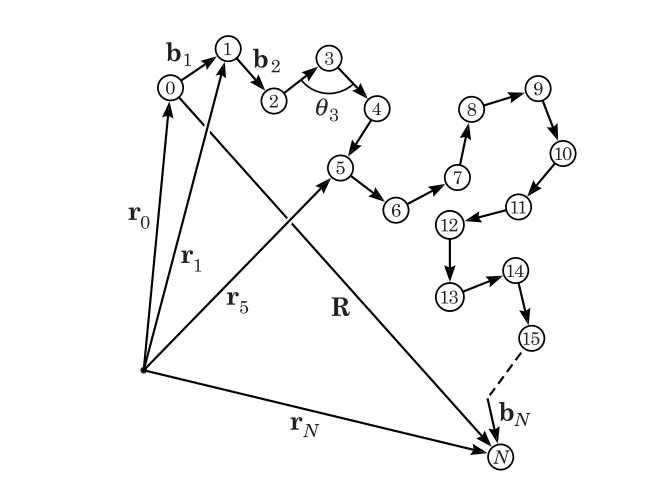
\includegraphics[scale=0.5
]{Contents/chapter2/figures/2-1.png}
\caption{粗粒链模型实例}
\end{figure}

此为由$N+1$个粒子与$N$个弹簧组成的粗粒链模型,粒子位置记为$\mathbf{r_0},……,\mathbf{r_N}$,键向量记为$\mathbf{b_1},……,\mathbf{b_N}$,链的端点间的向量记为$\mathbf{R}$。图中由2、3、4粒子的相互作用导致的$\theta_3$的角度限制就是一种近程干扰,而粒子6和12之间的穿透空间相互作用正说明了一种远程干扰。
从而,我们可以引出以下重要概念:
\begin{itemize}
	\item 真实链:考虑近程干扰和远程干扰的分子链。
	\item 理想链:仅考虑近程干扰而不考虑远程干扰的分子链。
\end{itemize}

有一个重要发现表示,不考虑近程干扰的特定形式,所有的理想链模型在足够大的长度范围内都具有普遍的缩放效应。为了更好的说明以上效应,考虑聚合物线圈的平均长度,$R=\sqrt{<\mathbf{R}\cdot \mathbf{R}>}$,其中$\mathbf{R}$为连接聚合物两端点的向量,符号$<……>$表示聚合物的全部构象态的平均值。从而,圈长$R$,即端点间向量的均方根,与聚合度N的关系如下
\begin{equation}
R \sim b N ^ { \nu } , \nu = 1 / 2 , \quad N \rightarrow \infty
\end{equation}
不考虑聚合物的化学细节和建模中使用的粗粒化水平,以上渐近比例关系中比例系数$\nu = 1/2$是通用的。非常值得注意的是,无论聚合物是聚苯乙烯还是聚乙烯,将聚合物链的分子量曾为四倍,聚合物线圈的平均尺寸就会增加一倍。相比之下,$(1)$式中作为前因子出现的长度尺度$b$(通常约为1nm)对聚合物的化学结构和粗粒化程度均敏感,但对总分子量不敏感。这个渐近极限的方法不是普遍的,它取决于近程干扰的范围。

从而我们考虑一个自然的问题,在什么条件下真实聚合物链满足$(1)$式中理想的链缩放定律?由于所有只有近程干扰的聚合物都表现出渐近理想的链缩放,这个问题可以转换为,在什么条件下真实链可以忽略远程干扰?令人好奇的是,线性均聚物在良好溶剂中无限稀释时的最简单情况并不遵循理想的链比例关系。

原则上,远程干扰永远不会完全消失。然而,通常会遇到两种情况,在这种情况下,远程干扰基本上可以忽略不计:
\begin{itemize}
	\item theta温度下高分子量均聚物的稀溶液。
	($\theta$态指溶液中高分子的链收缩和扩张力达到平衡,或溶剂与链段和链段与链段相互作用达到平衡,从而表观上呈现理想溶液的状态)
	\item 嵌在化学上相同的均聚物熔体中的均聚物链。
\end{itemize}

在排除了在空间上封闭但距离较远的聚合物段之间的体积相互作用的系统中,沿着这条链生成一个新的缩放行为的“通用性类”——即自避免随机游走:
\begin{equation}
R \sim b _ { s } N ^ { \nu } , \nu = 0.588 \ldots , \quad N \rightarrow \infty
\end{equation}
同样的,指数$\nu$是通用的,只取决于空间的维数(三维空间中$ v = 0.588 \dots$,二维空间中$ v =3/4 $),长度尺度$b_s$依赖于聚合物和溶剂的化学细节,但与聚合物分子量无关。
随着聚合物溶剂质量的降低(通常通过降低温度),聚合物段间的相互吸引作用通过溶剂介质传递。在$\theta$温度下,这些吸引相互作用正好补偿了排斥体积斥力,恢复了$(1)$式中的理想的链比例关系。

同样的现象也发生在均聚合物熔体中:两个聚合物段沿着同一条链远离,但在空间中间隔较短(约0.5 nm),它们之间的互斥很强。然而,这种净斥力在渐近极限过程中被许多其他的链(约有$N^{1/2}$个)抵消(“屏蔽”),这些链突出到兴趣链的随机线圈中。聚合物在相同聚合物熔体中的理想状态有时被称为弗洛里定理。

在这两种特殊情况以外的物理情况下,远程干扰通常在真实聚合物链的统计力学中起着重要的作用,应该通过指定合适的段间电位,将其纳入原子模型和介观模型中。我们将在第4章中看到,在构建粗粒度聚合物模型时,分离造成近程和远程干扰的相互作用是很方便的。此外,这种分离将产生聚合物场理论,其中单链模型的统计力学起中心作用。

读者可能已经注意到,对于在$(1),(2)$式中作为前置因子出现的非普遍长度$b$和$b_s$的物理解释一直相当模糊。粗略地说,我们可以把b看作是链的局部刚度损失和聚合物链的柔韧性首次显现的长度尺度。它与聚合物的键合约束的联系将在下面的具体理想链模型的背景下进行探讨。

\section{自由连接链模型}
{\color{red}\begin{center}
        刘玲
    \end{center}}

\begin{figure}[H]
	\centering   
	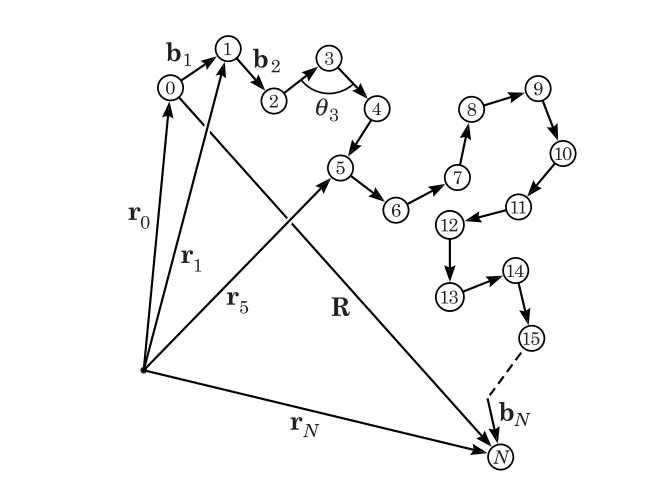
\includegraphics[width=12cm]{Contents/chapter2/figures/2-1.png}
	\caption{ }
    \label{fig:2.1}
\end{figure}

对于一般含$N+1$个粒子的粗粒聚合物模型,如图(\ref{fig:2.1})所示,单个链的构象配分函数(配分函数是一个平衡态统计物理学中经常应用到的概念,经由计算配分函数可以将微观物理状态与宏观物理量相互联系起来,而配分函数等价于自由能,与路径积分在数学上有巧妙的类似。)可以用类似$Z=\int \exp[-\beta U(\br^{n})] d \br^{N+1}$(1.6)的表示:\\
\begin{equation}
Z_0 = \int \exp[-\beta U_{0}({\br}^{N+1})] ~d \br^{N+1}
\label{2.3}
\end{equation}
其中$\br^{N+1}=(\br_0,\br_1,\ldots,\br_{N})$表示$N+1$粒子的位置,$U_0(\br^{N+1})$是与聚合物特定构型相关联的势能(下标$0$用来表示我们正在讨论单个理想链的性质)。$\int d\br^{N+1}$是三维区域内$N+1$粒子所占体积积分的缩写。对于理想链模型,$U_0$只包含反映短程干扰的相互作用势项。\\

在构象空间中观测点$\br^{N+1}$的联合概率密度是波尔兹曼(Boltzmann)分布(也叫吉布斯分布,是一种覆盖系统各种状态的概率分布、概率测量或者频率分布。当有保守外力(如重力场、电场等)作用时,气体分子的空间位置就不再均匀分布了,不同位置处分子数密度不同。玻尔兹曼分布律是描述理想气体在受保守外力作用、或保守外力场的作用不可忽略时,处于热平衡态下的气体分子按能量的分布规律):\\
\begin{equation}
P_0(\br^{N+1})=Z_{0}^{-1} \exp[[-\beta U_{0}(\br^{N+1})]
\label{2.4}
\end{equation}
此概率权重(或密度)被规范化,以便$\int P_0(\br^{N+1}) d\br^{N+1}=1$。在链的所有配置上,任意函数$f(\br^{N+1})$的系综平均值可以写成\\
\begin{equation}
\langle f(\br^{N+1})\rangle _0 =  \int P_0(\br^{N+1})f(\br^{N+1})~d\br^{N+1}
\label{2.5}
\end{equation}
另一种表示$N+1$粒子链构象自由度的方法是保留一个描述聚合物整体位置的“外部”坐标和N个“内部”坐标。一个特别方便的选择是链端的位置,例如,以及图2.1所示的N 个键向量,$\bb^{N}=(\bb_1,\bb_2,\ldots,\bb_{N})$,其中$\bb_{i}=\br_{i}-\br_{i-1}$。在聚合物没有外部势作用的情况下,$U_0$只依赖于内部坐标$\bb^{N}$。将$\br^{N+1}$和$(\br_0,\bb^{N})$ 进行雅克比变换,(\ref{2.3}-\ref{2.4})可重新表示为\\


\begin{equation}
Z_0 = V \int \exp[-\beta U_{0}(\bb^{N})]~d\bb^{N}
\label{2.6}
\end{equation}
\begin{equation}
P_0(\br_0,\bb^{N})=Z_{0}^{-1} \exp[[-\beta U_{0}(\bb^{N})]
\label{2.7}
\end{equation}
因此,在链端位置$\br_0$分布是均匀的。\\

自由连接链模型是一种非常简单的理想链模型,其中连接连续粒子的键向量被约束为一个固定的长度,$|\bb_{i}|=b$,但N个键向量的方向是各向同性独立分布的。在无限刚性弹簧的极限情况下,$U_0(\bb^{N})$的弹簧模型原则上可以实现固定键长的约束。一个更简单的方法是采用一个$\bb^{N}$表示法,这样约束就会自动得到满足。另
$\bb_{i}=b\bm{n}_{i}$,其中$\bm{n}^{N}=(\bm{n}_1,\bm{n}_2,\ldots,\bm{n}_{N})$是单位球面上一组均匀独立分布的N个单位向量。因此,对于自由连接链模型\\

\begin{equation}
P_0(\br_0,\bm{n}^{N})=\frac{1}{V} (\frac{1}{4 \pi})^{N}
\label{2.8}
\end{equation}
它是规范化的,所以$\int d\br_0\int P_0(\br_0,\bm{n}^{N})d\bm{n}^{N}=1$,其中$\int d\bm{n}^{N}$表示单位球面上的N个积分。\\
应用上式,我们可以检验自由连接链的各种统计性质。特别是端到端向量$\bbR=\br_{N}-\br_0$的矩,还可以写为$\bbR=\sum _{i=1}^{N} \bb_{i}=b \sum _{i=1}^{N} \bm{n}_{i}$.
$\bm{n}_{i}$的各向同性分布意味着$\langle \bm{n}_{i}\rangle _{0}=0$,因为在每点概率相同,$\bm{n}_{i}$分布在各个方向上,相互抵消,因此R的一阶矩消失\\
\begin{equation}
\langle \bbR \rangle_{0}=0
\label{2.9}
\end{equation}
端到端的二阶矩可以写出来\\
\begin{equation}
\langle \bbR_{\alpha} \bbR_{\beta}\rangle_{0}=b^2 \sum _{i=1}^{N} \sum _{j=1}^{N} \langle n_{i \alpha},n_{j \beta} \rangle_{0}
\label{2.10}
\end{equation}
这里我们用希腊下标来表示向量和张量的笛卡尔分量。当$i\neq j$双和项由于各单位向量的独立性而明显消失。对角线项用$\langle n_{i \alpha},n_{j \beta} \rangle_{0}=(1/3)\delta_{\alpha  \beta }$计算,其中$\delta_{\alpha \beta }$是克罗内克(Kronecker)符号,因此:\\
\begin{equation}
\langle \bbR_{\alpha} \bbR_{\beta}\rangle_{0}=\frac{b^{2}N}{3}\delta_{\alpha \beta }
\label{2.11}
\end{equation}
所以自由连接链模型的均方端到端向量完全符合理想链标度定律$R~bN^2,\nu=1/2,N \rightarrow \infty $(2.1):\\
\begin{equation}
R\equiv \sqrt{\langle \bbR \cdot \bbR\rangle _{0}}=bN^{1/2}
\label{2.12}
\end{equation}
注意,上式是在不施加$N\rightarrow \infty$的情况下导出的,(2.1)中省略的标度系数对于自由连接链是完全统一的。\\

端到端向量的更高矩也可以同样计算出来。例如\\
\begin{equation}
\langle (\bbR \cdot \bbR)^2 \rangle_{0}=\frac{5}{3}b^4N(N-\frac{2}{5})
\label{2.13}
\end{equation}
从这个结果可以看出,自由连接链的端到端向量$\bbR$的概率分布不是简单的高斯分布,因为对于这种分布(见附录B)$\langle (\bbR \cdot \bbR)^2 \rangle=\langle (\bbR \cdot \bbR) \rangle^2+2\langle (\bbR \bbR)\rangle:\langle (\bbR \bbR)\rangle$,这导致$\langle (\bbR \cdot \bbR)^2 \rangle_{0}=(5/3)b^4N^2$。但是,对于$N\rightarrow \infty$,上式中给出的四阶矩与高斯分布是一致的。\\

衡量聚合物链平均尺寸的另一个重要指标是回转半径$R_{g}$。这个量是单个片段(粒子)与聚合物质心之间的均方距离,$\bbR_{c}=(N+1)^{-1} \sum _{i=0}^{N} \br_{i}$,即\\
\begin{equation}
R_{g}^2 \equiv \frac{1}{N+1} \sum _{i=0}^{N} \langle (\br_{i}- \bbR_{c})^2 \rangle_{0} 
\label{2.14}
\end{equation}
因此$R_{G}^2$代表了质量分布在聚合物线圈中的二阶矩,而且还可以定义为所有聚合物的结构,例如没有链端的环状聚合物。旋转的平方半径可由另一种形式表示\\
\begin{equation}
R_{g}^2=\frac{1}{(N+1)^2} \sum _{i=0}^{N} \sum _{j>i}^{N} \langle (\br_{i}- \br_{j})^2 \rangle_{0} 
\label{2.15}
\end{equation}
这公式特别容易计算。还可以通过将$\br_{i}-\br_{j}$表示为键向量之和来计算自由连接链的表达式,从而得到$\langle (\br_{i}- \br_{j})^2 \rangle_{0}=b^2 |i-j|$。然后对上式中的二重和进行渐近求和,使$N \rightarrow \infty $。\\
\begin{equation}
R_{g}^{2} = \frac{b^2}{(N+1)^2} \sum _{k=1} ^{N} (N+k-1)k=\frac{b^2 N(N+1)(N+2)}{6(N+1)^2}
\end{equation}
\begin{equation}
R_{g}\approx b(N/6)^{1/2}
\label{2.16}
\end{equation}
因此,自由连接链的回转半径比均方端到端向量R小$1/\sqrt{6}$。这证明了在N足够大时线性聚合物的任何理想链模型都是成立的。\\
\begin{figure}[H]
	\centering   
	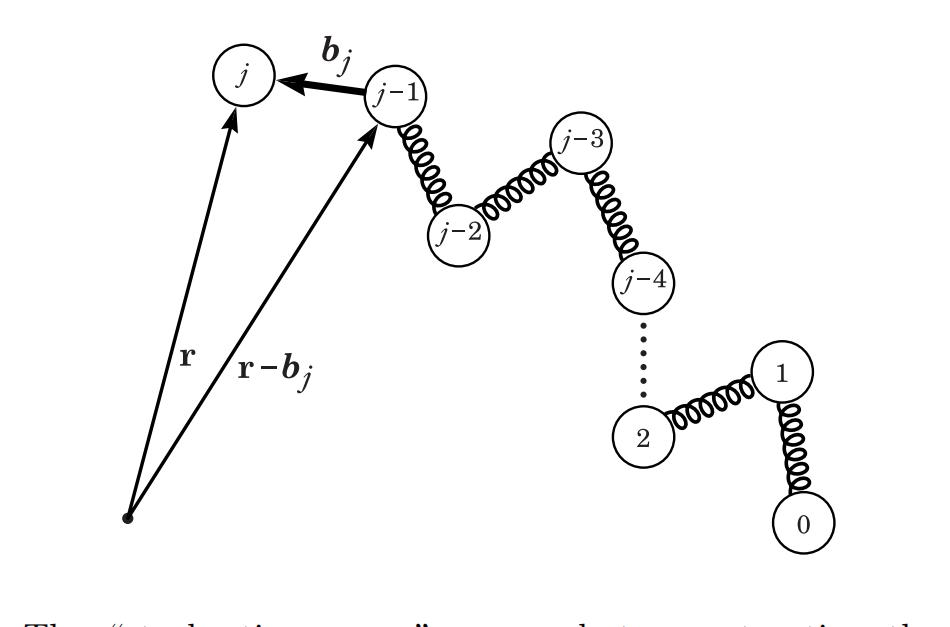
\includegraphics[width=12cm]{Contents/chapter2/figures/3.png}
	\caption{ }
	\label{2.2}
\end{figure}
图(\ref{2.2})从j个粒子链的统计权重出发,用“随机过程”方法建立具有j+1粒子的自由连接链末端位置的统计权重。\\

另一种探索理想链模型统计特性的方法不是计算矩,而是直接检测诸如端到端向量等量的概率分布函数。特别是约化分布函数$p_{0}(\br,j)$,它表示含有$j+1$个粒子的聚合物链在其末端r位置(粒子标记的j)的概率密度。该函数被规范化,以便$\int p_0(\br,j)d\br=1$。在构造这一目标时,我们将有机会在聚合物统计力学与随机过程理论之间建立一个重要的联系。具体来说,连续粒子沿粗粒聚合物链的随机位移类似于离散时间随机过程中在一定时间间隔内发生的随机事件。\\

为了利用随机过程的类比,我们假设一个含有较少粒子的链的末端$p_{0}(\br,j-1)$的概率密度是已知的,如图2.2所示,一个$(j+1)$粒子链可以通过添加一个粒子和一个连接键从j粒子链中建立。在自由连接链模型中,附加键的长度是固定的,但它的取向与链中已经存在的$j−1$个键的方向无关。因此,我们可以从已知的函数$p_{0}(\br,j)$乘以一个跃迁概率(与所加键的固定长度和均匀方向分布一致)求出概率密度,并对所有可能的键方向进行积分,\\
\begin{equation}
p_{0}(\br,j)=\frac{1}{4 \pi} \int p_0(\br-b \bm{n},j-1)d\bm{n}
\label{2.17}
\end{equation}
这个方程中的因子$1/(4 \pi)$表示与所加键的取向有关的均匀跃迁概率,积分又在单位球面上。这种方程在随机过程理论中称为查普曼-科莫高洛夫(Chapman-Kolmogorov)方程。在这里,自由连接链是一步马尔可夫过程的一个例子,因为跃迁概率只连接链上相邻的粒子。\\

对于解像(\ref{2.17})这样的方程,我们需要一个“初始条件”,指定一个1-粒子链的位置分布。然后依次迭代求出$(N+1)$-粒子链末端位置的概率密度$p_{0}(\br,N)$,这种递推格式非常适合于数值计算。就目前的目的而言,(\ref{2.17})可用于推导自由连接链的端到端向量的全部分布函数。\\

为了方便,引入函数$f(\br)$的三维傅里叶变换(与傅里叶分析有关的定义和公式在附录A中)\\
\begin{equation}
\hat{f}(\bk)=\int e^{-i\bk \cdot \br}f(\br)~d\br
\label{2.18}
\end{equation}
给出逆变换\\
\begin{equation}
 f(\br)=\frac{1}{(2 \pi)^3} \int e^{i\bk \cdot \br} \hat{f}(\bk)~d\bk
\label{2.19}
\end{equation}
将傅里叶变换应用于(\ref{2.17})的两边,得到以下表达式:\\
\begin{equation}
\begin{aligned}
\hat{p_0}(\bk,j)&=\frac{1}{4 \pi} \int e^{-ib\bk \cdot \bm{n}} \hat{p_0}(\bk,j-1)d\bm{n} \\&=\frac{1}{4 \pi} \int _{R^3}e^{-ib\bk \cdot \bm{n}} \hat{p_0}(\bk,j-1)d\bm{n} \\&=
\frac{1}{4 \pi} \int _{0}^{2 \pi}d \varphi \int _{0}^{\pi} e^{ib|\bk|\bm{n} cos \theta}sin \theta d \theta \hat{p_0}(\bk,j-1) \\&=\frac{1}{2} \int _{-1}^{1}cos b|\bk|dx \hat{p_0}(\bk,j-1) \\&=j_0(b|\bk|)\hat{p_0}(\bk,j-1)
\label{2.20}
\end{aligned}
\end{equation}
其中$j_0(x) \equiv (sinx)/x$是常见的球面贝塞尔函数。依次地将这个方程应用于$j=1,2,\ldots,N$得到\\
\begin{equation}
\hat{p_0}(\bk,N)=[j_0(b|\bk|)]^{N}\hat{p_0}(\bk,0)
\label{2.21}
\end{equation}
特别有趣的情形是对应于初始条件$p_0(\br,0)=\delta(\br)$,其中$\delta(\br)$是三维狄拉克函数(狄拉克函数是由性质定义的广义函数,对于任何函数成立,另见附录A)。这意味着链的起始端(粒子$0$) 被约束于原点。有了这种选择,$\hat{p_0}(\bk,0)=1$,$p_0(\bbR,N)$可以解释为含有$N$个键和端到端向量的自由连接链的概率密度。因此\\
\begin{equation}
p_0(\bbR,N)=\frac{1}{(2 \pi)^3 }\int e^{i\bk \cdot \bbR}[j_0(b|\bk|)]^{N}d\bk
\label{2.22}
\end{equation}
是端到端向量的概率密度的精确闭型表达式。当$N\gg1$且$|\bbR| \ll Nb $时,对这个积分的渐近分析证实了我们先前观察到的$\bbR$的二阶和四阶矩与高斯分布是一致的。\\
\begin{equation}
p_0(\bbR,N) \approx [3/(2 \pi Nb)]^{3/2}exp[-3|\bbR|^2/(2Nb^2)]
\label{2.23}
\end{equation}
构象熵的重要概念体现在上式中。在自由连接链的全相空间分布函数$P_0(\br_0,\bb^{N})$与端到端向量的约化概率分布函数$p_0(\bbR,N)$转换的过程中,我们固定端到端向量$\bbR=\sum _{i=1}^{N} \bb_{i}$,在所有固定长度键向量$b$上进行了积分。这种集成相当于对构象状态的枚举。由于在自由连接的模型中,所有的状态都以均匀的概率发生,所以结果是对约束端到端向量$\bbR$的链的自由能的纯粹熵表现:\\
\begin{equation}
F_0(\bbR)=-k_{B}Tlnp_0(\bbR,N)\approx \frac{3k_{B}T}{2Nb^2}|\bbR|^2
\label{2.24}
\end{equation}
这个表达式中的二次项依赖于链的扩张维R可以看作是一个“熵弹簧”势。对于具有较大扩展的链,可用的构象态较少,因此自由能随的增加而增加。此外,$\frac{3k_{B}T}{Nb^2}=\frac{k_{B}T}{2R^2_{g}}$的“弹簧常数”与聚合物线圈尺寸的平方成反比。\\

最后一个主题涉及到自由连接链模型在理想条件下对真实链的适用性。在短尺度(约$1nm$)上,自由连接链明显地简化了真实聚合物链的键合和空间约束,该链仅在一定距离b上包含局部键刚性。然而,在较大的尺度上,即$5~10nm$,真实的柔性聚合物在理想状态下表现出符合(\ref{2.12})的自由连接链的标度行为。因此,我们可以通过定义一个等效的自由连接链来描述这类聚合物的介观统计特性。即要求处于理想状态的真实聚合物具有相同的均方端到端向量$R^2=Nb^2$,最大端到端距离$\bbR_{max}=Nb$作为等效的自由连接链。然后,自由连接链的两个参数可以用实验测量或$R^2=\langle \bbR \cdot \bbR\rangle_{0}$和$R_{max}$的估计来表示\\
\begin{equation}
b=R^2/R_{max},N=R_{max}^{2}/R^2
\label{2.25}
\end{equation}
按照这一程序,等价链的键长$b$称为库恩段长度,对大多数乙烯基聚合物而言约为$1nm$。等价链的有效“库恩段”的个数$N$通常比实际链的骨架键数小$50$倍。\\

显然,(\ref{2.25})中给出的将理想状态下的真实链映射到自由连接模型上的条件并不是唯一的。高度扩展的链构象是非常罕见的,因此在实链和等价链之间匹配$R_{max}$的理由是很弱的。定义等效自由连接链的其他方法通常涉及$N$的定义,然后通过匹配实链和等价链之间的$R^2$(或$R_{g}^{2}$)来计算$b$。$N$的一般定义包括每条链的单体重复单位的平均数目,或每条具有规定分子量的链段的平均数目(这可能与实际的化学重复单位相对应,也可能不对应)。从这些过程中获得的$b$值通常称为统计段长度。需要注意的是,$b$和$N$的值将因定义等价链所用的标准而有所不同。然而,所建立的链模型一般都能很好地描述真实聚合物链在理想状态下的介观$(1nm)$统计特性,而不考虑所应用的准则。\\

在本专著中,我们将采用一种比较随意的语言来引用粗粒度、等价链模型中的参数。$n$将可互换地描述为聚合度、每个链的单体数或统计段数。同样,$b$将被称为库恩长度,统计段长度,或单体长度。\\



\endinput

\subsection{珠弹簧(bead-spring)模型}
\begin{center}
\author{何志娟}
\end{center}


另一类要的理想链模型是所谓的珠弹簧模型,在这些模型中,沿粗粒链的连续粒子被“弹簧电势(spring potentials)”所束缚,这些弹簧电势有多种形式被选择。定义这些模型的势能$U_{0}$是最合适表达键向量的术语。因此,配分函数和相空间分布函数的$(N+1)$个粒子链(见图\ref{2.1})通常被写成公式(\ref{2.6})-(\ref{2.7})的形式。如果这样一个链的$N$键全部等价和没有外场的干扰,这些势能可以表示为:
\begin{equation}\label{2.26}
U_{0}(\bb^{N})= \sum_{i=1}^{N}h(|\bb_{i}|)
\end{equation}
其中$h(x)$是沿高分子聚合物相邻粒子的弹簧电势,因此得出的结论是:
\begin{equation}\label{2.27}
Z_{0}=V(\int \exp[-\beta h(|\bb|)]~d\bb)^N 
\end{equation}
\begin{equation}\label{2.28}		
P_{0} (r_{0},\bb^N) =V^{-1} \prod_{i=1}^{N} \frac{\exp[-\beta h(|\bb_{i}|)]}{\int \exp[-\beta h(|\bb_{i}|)]~d \bb_{i}}
\end{equation}
因此,每个键向量$\bb_{i}$都是独立分布的,其统计权重与$\exp[-\beta h(|\bb_{i}|)]$成正比。 

它仍然需要指定键$h$弹簧电势的函数形式。最常见的选择是定义所谓的离散高斯链模型的谐波键电势(harmonic bond potential): 
\begin{equation}\label{2.29}
h(x)=\frac{3k_{B}T}{2b^2} x^2  
\end{equation}
这个电势的参数$b$,可以被理解为键的均方根长度,因为对任意键$i$
\begin{equation}\label{2.30}
\begin{aligned}
<\bb_{i}.\bb_{i}>_{0}&= \frac{\int_{-\infty}^{\infty} (\bb_{i}.\bb_{i})~\exp[-\beta h(|\bb_{i}|)])~d\bb_{i}}{\int_{-\infty}^{\infty} \exp[-\beta h(|\bb_{i}|)]~d\bb_{i}}\\ &=\frac{\int_{-\infty}^{\infty}\int_{-\infty}^{\infty}\int_{-\infty}^{\infty}(x_1^2+x_2^2+x_3^2)~\exp[{-\frac{3}{2b^2}(x_1^2+x_2^2+x_3^2)}]~dx_1dx_2dx_3}{\int_{-\infty}^{\infty}\int_{-\infty}^{\infty}\int_{-\infty}^{\infty}~\exp[{-\frac{3}{2b^2}(x_1^2+x_2^2+x_3^2)}]~dx_1dx_2dx_3}\\ &=\frac{3\int_{-\infty}^{\infty}\int_{-\infty}^{\infty}\int_{-\infty}^{\infty}~x_1^2~\exp[{-\frac{3}{2b^2}(x_1^2+x_2^2+x_3^2)}]~dx_1dx_2dx_3}{\int_{-\infty}^{\infty}\int_{-\infty}^{\infty}\int_{-\infty}^{\infty}~\exp[{\frac{-3}{2b^2}(x_1^2+x_2^2+x_3^2)}]~dx_1dx_2dx_3}\\ &=\frac{3 \times\frac{1}{2} (\frac{2b^2}{3})^{3/2}\sqrt{\pi}}{(\frac{2b^2\pi}{3})^{\frac{1}{2}}}\\ &=b^2
\end{aligned}
\end{equation}
其中,所需的高斯积分是附录B中给出的公式的。

离散高斯链的均方端到端向量可以类似的计算,特别的:
\begin{equation}\label{2.31}
<\bbR\cdot\bbR>_{0}=\sum_{i=1}^{N}\sum_{i=1}^{N}<\bb_{i}\cdot\bb_{i}>_{0}
\end{equation}
在这个表示当中,当$i\neq j$时,独立分布的键向量不存在,当$i\neq j$时,$<\bb_{i}\cdot\bb_{j}>_{0}=<\bb_{i}>_{0}<\bb_{j}>_{0}=0$。因此
\begin{equation}\label{2.32}
<\bbR\cdot\bbR>_{0}=N<\bb_{i}\cdot\bb_{i}>_{0}=Nb^2
\end{equation}
并精确的恢复了公式((\ref{2.12})的理想链标度,$R=bN^\frac{1}{2}$,除了将$b$作为自由连接模型固定键长与离散高斯模型的均方根外,我们发现这两个理想模型均方端到端向量的表达是一致的。这容易证明回璇半径$R_{g}$是等价的。因此公式(\ref{2.16})也可以适用离散高斯链。
\begin{figure}[H]
\centering
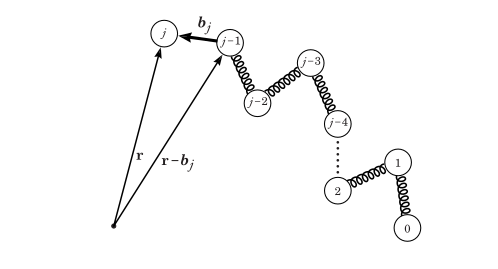
\includegraphics[width=15cm]{Contents/chapter2/figures/23.png}
\caption{"随机过程”方法构造离散高斯链的末端的统计权重,其中j+1粒子来自j粒子的统计权重。}
\label{figures23}
\end{figure}


为了更充分的探索自由链接和离散高斯链模型的关系,利用随机过程的联系是非常有用的。关于自由连接链,我们考虑约化分布函数$P_{0}(\br,j)$,表示在$\br$位置观察(j+1)--粒子链末端粒子j的概率密度。假设一条链的概率密度比它少一个粒子$p_{0}(\br,j-1)$,如图\ref{figures23}所示,通过Chapman-Kolmogorov公式建立:
\begin{equation}\label{2.33}
P_{0}(\br,j)=\int  \varPhi (\bb_{j};\br-\bb_{j})~p_{0}(\br-\bb_{j},j-1)~d\bb_{j}
\end{equation}
在这个表达式中$\varPhi (\bb_{j};\br-\bb_{j})$是连续粒子$j$和$j-1$键向量假设在$\bb_{j}$的条件概率密度,给出粒子$j-1$在$\br-\bb_{j}$位置。这是规范化的,因此$\int  \varPhi (\bb_{j};\br-b\bb_{j})~d\bb_{j}=1$。不在任何外场的离散高斯链,$\varPhi$是链上粒子指数j(即随机过程是“平稳的”)和起始位置$\br-\bb_{j}$上独立,因此,条件转移概率密度只反映键位移的高斯分布:
\begin{equation}\label{2.34}
\begin{aligned}
\varPhi(\bb_{j};\br-\bb_{j})=\varPhi(\bb_{j})&=\frac{\exp[-\beta h(|\bb_{j}|)]}{\int \exp[-\beta h(|\bb_{j}|)]~d\bb_{j}} \\ &=(\frac{3}{2 \pi b^2})^{\frac{3}{2}}~\exp[-3|\bb_{j}|^2 / (2b^2)]
\end{aligned}
\end{equation}
公式(\ref{2.33})易于用Fourier变换求解,因为离散高斯链$\varPhi$转移概率形式意味着右边是一个三维的卷积积分公式(见附录A)。因此公式(\ref{2.33})的Fourier变换得到Fourier变换的乘积
\begin{equation}\label{2.35}
\hat{p}_{0}(\bk,j)=\hat{\varPhi}(\bk)\hat{p}_{0}(\bk,j-1)
\end{equation}
对$j=1,2,\dots ,N$归纳递推得:
\begin{equation}\label{2.36}
\hat{p}_{0}(\bk,N)=[\hat{\varPhi}(\bk)]^N\hat{p}_{0}(\bk,0)
\end{equation}
公式(\ref{2.34})中的高斯转移概率的Fourier变换是高斯的$^{11}$。$\hat{\varPhi}(\bk)=\exp(-b^2|\bk|^2/6)$,因此公式(\ref{2.36})的离散高斯链可以化简为:
\begin{equation}\label{2.37}
\hat{p}_{0}(\bk,N)=\exp(-R_{g}^2|\bk|^2)\hat{p}_{0}(\bk,0)
\end{equation}
这里写$R_{g}=\sqrt{Nb^2/6}$作为链的回旋半径来计算,最后,我们专门讨论粒子0约束原点$p_{0}(\br,0)=\delta(\br)$的情况。其中$\hat{p}_{0}(\bk,0)=1$,则公式(\ref{2.37})的Fourier逆变换可以写成:
\begin{equation}\label{2.38}
p_{0}(\bbR,N)=[3/(2\pi Nb^2)]^\frac{3}{2}\exp[-3|\bbR|^2/(2Nb^2)]
\end{equation}

将离散高斯链的这些结果和自由连接链的结果进行比较是很有意思的,特别的,我们发现自由连接链模型公式(\ref{2.21})的精确分布函数$\hat{p}_{0}(k,N)$的Fourier变换与离散高斯链公式(\ref{2.37})不一致,但是对于长度超过b,如:$b|k|<<1$,
\begin{equation}\label{2.39}
[j_{0}(b|\bk|)]^N\approx [1-b^2|\bk|^2/6+\dots]^N\approx \exp(-R_{g}^2|\bk|^2)
\end{equation}
这两个函数是一致符合的。观察的结果是离散高斯链公式(\ref{2.38})是精确的,但是对于自由链接链的结果是近似的(要求$N>>1$且$|\bbR|<<Nb$)。

离散高斯连模型只是众多可设计的珠弹簧模型之一。这是个特别方便的模型,因为在粗粒键和介观端到端向量的水平上都是高斯的段分布,这便于分析计算各种各样单链的性能。然而,利用连接键的调和势(harmonic potential)的线性(Hookian)弹簧模型有时是不够的。例如:高斯链模型在描述低盐条件下(Netz and Orland,1999)的电解质时,可以表示较大的非物质拉伸。具有延伸特性强的流体力学流动作用下的高斯链也不能代表真实聚合物的无限延伸(Larson,1986)。在这种情况下,可以利用非线性的弹簧模型来防止非物质的扩展链现象。自由连接链也可以被应用,但是由于与固定键长度相关的完整性约束在动态高分子聚合物方案中往往更难实现。(Doi and Edwards,1986).

大部分非均匀聚合物的计算是通过数值计算的观点来实现的,目前使用非线性的珠弹簧模型比较容易,特别是公式(\ref{2.36})适用于所有键相同且其特点是仅取决于键长x的弹簧电势h(x)的任何珠弹簧。$\varPhi(\bk)$的形式是区分不同链模型的统计特征。一般情况下h(x)的转移概率密度的Fourier变换可以被写为:
\begin{equation}\label{2.40}
\hat{\varPhi(\bk)}=\frac{\int_{0}^{\infty}  x^2j_{0}(|\bk|x)\exp[-\beta h(x)]~dx}{\int_{0}^{\infty}  x^2\exp[-\beta h(x)]~dx} 
\end{equation}
对于公式(\ref{2.29})的线性(高斯)弹簧模型$\hat{\varPhi(k)}=exp(-b^2|k|^2/6)$。比较公式(\ref{2.21})和(\ref{2.36})表明自由连接链模型可以类似的表示:$\hat{\varPhi_{FJ}(k)}=j_{0}(b|k|)$。

作为非线性的珠弹簧模型的例子,考虑类似流变学的计算Warner spring的电势:
\begin{equation}\label{2.41}
h(x)=\frac{2k_{B}T}{2b^2}\frac{x^2}{(1-x^2/b_{0}^2)}
\end{equation}
此电势包含的参数$b_{0}>0$即当$h(x)\to +\infty,x\to b_{0}$键的最大长度,但是,对于弱键的扩张$x/b_{0}<<1$公式(\ref{2.41})减到公式(\ref{2.29})中给定的调和键位电势。因此公式(\ref{2.41})是双参数非线性弹簧定律。它与离散高斯链模型中小键位移的线性定律一致。然而,对于强作用力键长在有限的$b_{0}$处是饱和的。

当被替换公式(\ref{2.40})时,公式(\ref{2.41})的非线性性弹簧模型会导致转换后的转移概率密度$\varPhi_{NL}(k)$可以表示为(wavevector)波矢量和无尺度$b/b_{0}$比的函数,对于$b/b_{0}<0.1$,$\varPhi_{NL}(b|k|,b/b_{0})$与线性弹簧函数$\varPhi_{G}(k)$几乎没差别。 然而,当$b/b_{0}$的值比较大时,非线性弹簧在波矢量中的影响依赖于$\varPhi_{NL}(k)$。图\ref{figures24}比较了离散高斯链、自由连接链和公式(\ref{2.41})的非线性珠弹簧链在$b/b_{0}=1$情况下的转移概率的Fourier变换。非线性弹簧定律对$|k|$具有振幅依赖性,其性质上类似于自由连接链。然而,自由链接模型振幅受到更强的阻尼,其键的长度被严格地约束为$b$。
\begin{figure}[H]
\centering
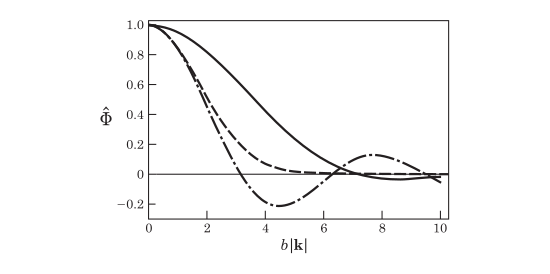
\includegraphics[width=15cm]{Contents/chapter2/figures/24.png}
\caption{分别是离散高斯(虚线),自由连接链(点虚线)和非线性弹簧模型(实线)的键转移概率$\varPhi_{G}$、$\varPhi_{Fj}$和$\varPhi_{NL}$的Fourier变换,用$b/b_{0}=1$来计算非线性弹簧模型}
\label{figures24}
\end{figure}

\subsection{连续高斯链模型}
\begin{center}
龚欣
\end{center}

连续高斯链是一种用于分析和数值计算的理想链模型(Doi和Edwards),该模型可以被视为离散高斯链模型的连续极限,其中的聚合物被视为一个连续的线性弹性丝(linearly elastic filament)。如图\ref{空间曲线描述聚合物构型}所示,连续高斯链的构型由空间曲线$\br (s)$描述,表示高分子长链上某一链节的位置,其中$s\in [0,N]$,被定义为路径(contour)变量。第$s$个链节在空间中的位置记为$\br (s)$,端到端向量(end-to-end-vector)$R$可以表达为$R=\br (N)−\br (0)$。
\begin{figure}[H]
\centering
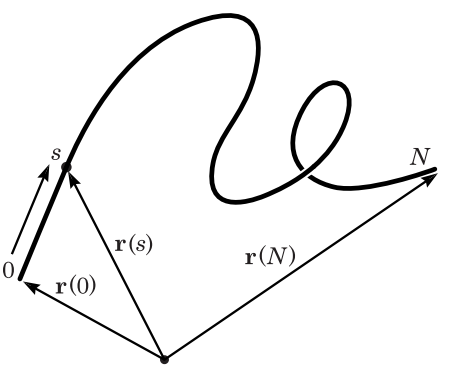
\includegraphics[scale=0.5]{Contents/chapter2/figures/41.png}
\caption{空间曲线$\br (s)$描述连续高斯链模型将聚合物的构型,其中$s\in [0,N]$是路径参数。$\br (0)$和$\br (N)$是链端位置。}
\label{空间曲线描述聚合物构型}
\end{figure}

连续高斯链的势能是
\begin{equation}
U_0[\br ]=\frac{3k_BT}{2b^2}\int_{0}^{N} \left| \frac{d\br (s)}{ds} \right|^2\mathrm{d}s \label{242}
\end{equation}
其中$U_0[\br ]$的方括号表示$U_0$是定义聚合物构型的空间曲线$\br (s)$的泛函。泛函是连续函数到数之间的映射(Volterra,1949),在上式中,这个映射是$\br (s)$与$U_0$值的关系。势能的形式与离散高斯链的方程$U_0(\bb ^N)=\sum_{i=1}^{N}h(\left|\bb _i\right|)$和$h(x)=\frac{3k_BT}{2b^2}x^2$密切相关。如果我们将$\frac{d\br (s)}{ds}$看作是高分子长链上第$s$节(链节长度为$ds$)的拉伸形变,则方程(\ref{242})是对链的整个路径上每一个这样的微分段的谐波势贡献(harmonic potential contribution)求和。值得注意的是,在连续高斯链模型中,$s$并不表示弧长,而只是表示链上各段的参数指标。因此,拉伸$\frac{d\br (s)}{ds}$不是固定的单位向量,它的大小是可以自由波动的。势能方程(\ref{242})通常称为“Edwards Hamiltonian”。

连续高斯链的构型配分函数是
\begin{equation}
Z_0=\int ~\exp(-\beta U_0[\br ])\calD \br  \label{243}
\end{equation}
其中$\int \calD \br $表示所有可能的描述聚合物的构型的空间曲线$\br (s)$上的泛函积分。这类泛函积分,又称路径积分,是量子力学和概率论领域(Feynman和Hibbs,1965)所熟悉的,其中$\br (s)$对应于量子粒子或布朗(Brownian)粒子在时间$s$时的位置。实际上,方程(\ref{243})在经典扩散(brownian motion)的路径积分中称为维纳测度(Wiener measure)。

路径积分是一种复杂的数学对象,在定义和操作上需要一定的精确性(Simon,1979)。然而在这里,我们将非正式地和以物理的方式来研究这些对象。定义路径积分有两种方法,其中一种方法是用$N_s+1$个等距路径点去离散路径,因此我们用$N_s+1$个点的空间位置逼近连续函数$\br (s)$,其中这$N_s+1$个点由向量$(\br _0,\br _1,...,\br _{N_s})$表示。这样,路径积分可以定义为$3(N_s+1)$维的普通积分(假设聚合物在体积为$V$的三维空间中)
\begin{equation}\label{244}
\int \calD \br \approx \prod_{i=0}^{N_s} \int \, \mathrm{d} \br _i
\end{equation}
其中,近似的质量随着$N_s$的增加而提高。当$N_s$有限时,连续高斯链的路径积分近似于有$N_s+1$个珠子的离散高斯链的配分函数。特别是,我们有一个近似
\begin{equation}\label{245}
Z_0=\lim_{N_s \to \infty} \prod_{j=0}^{N_s} \int \,\exp \left( -\frac{3}{2b^2\Delta s}\sum_{i=1}^{N_s}\left|\br _{i-1}-\br _i \right|^2 \right) \mathrm{d} \br _j 
\end{equation}
证明:
\begin{equation*}
\begin{aligned}
Z_0 &=\lim_{N_s \to \infty} \prod_{j=0}^{N_s} \int \,\exp\left(-\frac{3}{2b^2} \sum_{i=1}^{N_s} \int _{N_{i-1}}^{N_i} \left| \frac{\mathrm{b} \br  (s) } {\mathrm{d} s} \right|^2 \right) \mathrm{d} \br _j\\ 
& =  \lim_{N_s \to \infty} \prod_{j=0}^{N_s} \int \, \exp\left(-\frac{3}{2b^2}\sum_{i=1}^{N_s}\int _{N_{i-1}}^{N_i}\left|\frac{\br _{i-1}-\br _i}{\Delta s} \right|^2 \right)\mathrm{d} \br _j \\ 
&=  \lim_{N_s \to \infty} \prod_{j=0}^{N_s} \int \,~\exp \left( -\frac{3}{2b^2\Delta s}\sum_{i=1}^{N_s}\left|\br _{i-1}-\br _i \right|^2 \right) \mathrm{d} \br _j\\ 
\end{aligned}
\end{equation*}
其中一个$N_s$键的均方长度(mean-squared)由$b^2\Delta s$给出,$\Delta s=N/N_s$是路径点之间的间距。

方程(\ref{245})的巧妙之处源于连续极限,因为$Z_0$大小为$VN_s^{−(3/2)N_s}$,当$N_s\rightarrow \infty$时为零。通常我们对平均值感兴趣,它可以表示成两路径积分的比率。例如,连续高斯链的端到端向量的平方可以表示为
\begin{equation}\label{246}
R^2\equiv \left \langle \br \cdot \br \right \rangle _0=\frac{\int \left| \br (N)-\br (0) \right|^2~\exp(-\beta U_0[\br ]) \calD \br }{\int ~\exp(-\beta U_0[\br ]) \calD \br } 
\end{equation}
其中分母只是配分函数$Z_0$。当根据方程(\ref{246})对上述方程的分子和分母中的路径积分进行离散时,
发现奇异因子完全抵消,从而当$N_s\rightarrow \infty$时,$R^2$更好定义。此外,在路径积分的数值计算中,通常采用有限的$N_s$来避免奇异性。在整本书中,像方程(\ref{243})这样的表达式将以一种正式的方式被写和操作。我们应该意识到,在定义和估计这些对象时,可能确实存在一些微妙之处。

定义路径积分的另一种方法是通过路径的谱表示(spectral represention)。特别是,我们可以用扩充的一组完整的基函数$\lbrace \phi _0(s),\phi _1(s),... \rbrace$来表示空间曲线$\br (s)$
\begin{equation}\label{247}
\br (s)=\sum_{p=0}^{\infty} \ba _p \phi _p(s)
\end{equation}
这是一种广义的傅里叶展开式,其展开式系数$\ba _p$可以看作是广义傅里叶系数(见附录A)。对于在流体介质中自由悬浮(freely suspended in a fluid medium)的聚合物,基函数的一种方便的选择是符合“无拉伸”(no-stretch)边界条件的余弦集$\frac{d\br (s)}{ds}\vert _{s=0}=\frac{d\br (s)}{ds}\vert _{s=N}=0$。这相当于余弦傅里叶级数表示
\begin{equation}\label{248}
\br (s)=\ba _0+2\sum_{p=1}^{\infty} \ba _p \cos(p\pi s/N)
\end{equation}
根据这些基函数的正交性可以求解傅里叶系数
\begin{equation}\label{249}
\ba _p=\frac{1}{N}\int_{0}^{N} ~\cos(p\pi s/N)\br (s) \mathrm{d}s,p=0,1,2,...,\infty
\end{equation}
这些模型在聚合物文献中被称为Rouse模型,在聚合物动力学理论中起着特别重要的作用(Doi和Edwards,1986)。实际上,$\ba _0$可以解释为聚合物质心的位置,而$\ba _p,p=1,2,3,...$,尺度越细则提供更多关于聚合物形状的信息。

利用Rouse谱表示,聚合物的所有构型(路径)上的积分可以解释为对所有Rouse模型的积分的乘积。
\begin{equation}\label{250}
\int \calD \br = \prod_{p=0}^{\infty} \int \, \mathrm{d} \ba _p
\end{equation}
上述表达式右手边的对象是一个无穷维积分,所以我们再次遇到了配分函数$Z_0$的存在性问题。然而,这两个路径积分的比率是有限的,
为了数值计算的目的,我们取有限$P\gg1$使路径积分正则化(消除奇异点)
\begin{equation}\label{251}
\int \calD \br \approx \prod_{p=0}^{P} \int \, \mathrm{d} \ba _p\end{equation}
为了说明Rouse模型在连续高斯链计算中的应用,用Rouse模型表示端到端向量的平方值是
\begin{equation}\label{252}
\left | \br (N)-\br (0) \right |^2=16\sum_{p=1,3,...}^{\infty}\sum_{q=1,3,...}^{\infty} \ba _p \cdot \ba _q
\end{equation}
证明:
\begin{equation*}
\begin{aligned}
\left | \br (N)-\br (0) \right |^2 & =\left | 2\sum_{1}^{\infty}\ba _p\cos (p\pi)-2\sum_{1}^{\infty}\ba _p \right |^2\\ & =4\left | \sum_{1}^{\infty}\ba _p(\cos(p\pi)-1) \right |^2 \\ & =16\sum_{p=1,3,...}^{\infty}\sum_{q=1,3,...}^{\infty} \ba _p \cdot \ba _q\\
\end{aligned}
\end{equation*}
这个数的均值可以写为
\begin{equation}\label{253}
\left \langle \left| \br  \right|^2 \right \rangle _0=16\sum_{p=1,3,...}^{\infty}\sum_{q=1,3,...}^{\infty} \left \langle \ba _p \cdot \ba _q \right \rangle _0 
\end{equation}
其中,在Rouse模型中定义对象$f(\ba )$的均值为
\begin{equation}\label{254}
\left \langle f(\ba ) \right \rangle _0=\frac{\begin{matrix} \prod_{p=1}^{\infty} \int \,f(\ba )\exp(-\beta U_0(\ba )) \mathrm{d} \ba _p  \end{matrix}}{\begin{matrix} \prod_{p=1}^{\infty} \int \,\exp(-\beta U_0(\ba )) \mathrm{d} \ba _p  \end{matrix}}
\end{equation}
在Rouse模型表达式中,方程(\ref{242})的势能是对角的
\begin{equation}\label{255}
\beta U_0(\ba )=\frac{1}{2}\sum_{p=1}^{\infty}\alpha (p)\ba _p \cdot \ba _p
\end{equation}
其中$\alpha (p)=6\pi ^2p^2/(b^2N)$。注意,质心$p=0$模型是均匀分布。$p>0$模型都是统计独立的,是高斯分布,因此如下有(附录$B$)
\begin{equation}\label{256}
\left \langle \ba _p \cdot \ba _q \right \rangle _0=\frac{3}{\alpha (p)}\delta _{pq}
\end{equation}
替换到方程(\ref{246})将得
\begin{equation}\label{257}
\left \langle \left| \br  \right|^2 \right \rangle _0=\frac{8b^2N}{\pi ^2}\sum_{p=1,3,...}^{\infty}\frac{1}{p^2}=b^2N
\end{equation}
由此我们得出结论:连续高斯链具有离散高斯链的性质,它的端到端向量的均方值由$R=bN^{1/2}$给出。类似用期望公式给出连续高斯链的旋转半径$R_g=b(N/6)^{1/2}$。

\begin{figure}[H]
\centering
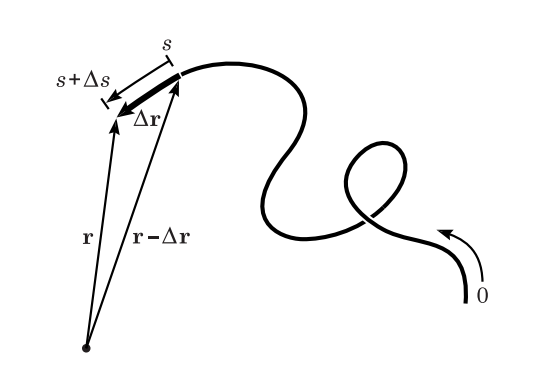
\includegraphics[scale=0.7]{Contents/chapter2/figures/42.png}
\caption{用“随机过程”(stochastic process)方法从具有$s$段的连续高斯链的统计权重中构造出具有$s+\Delta s$段的连续高斯链末端位置的统计权重。} \label{随机过程}
\end{figure}

在探索连续高斯链模型的性质时,我们现在回到了随机过程方法。具体来说,考虑一个约化的分布函数$p_0 (\br ,s)$是很有用的,它描述了在$\br$处,一个连续的路径长度为$s$的高斯链。这个函数满足归一化条件的,即$\int \,p_0(\br ,s) \mathrm{d} \br =1$。通过对离散高斯链的方程$p_0(\br ,j)=\int \,\Phi(\bb _j;\br -\bb _j)p_0(\br -\bb _j,j-1) \mathrm{d} \bb _j$的类比,我们可以通过Chapman-Kolmogorov方程利用非常小的链的信息建立分布函数
\begin{equation}\label{258}
p_0(\br ,s+\Delta s)=\int \,\Phi(\Delta \br ;\br -\Delta \br )p_0(\br -\Delta \br ,s) \mathrm{d}(\Delta \br ) 
\end{equation}

图\ref{随机过程}说明了上述方程的物理内容,它依赖于连续链的最后一部分离散化。转移概率密度$\Phi(\Delta \br ;\br -\Delta \br )$描述了路径长度$\Delta s$的链段的位移为$\Delta \br $的条件概率,从路径位置$s$处的$\br -\Delta \br $开始。连续高斯链的相关随机过程是稳定的,所以$\Phi =\Phi(\Delta \br )$与起始位置和路径位置无关。$\Phi(\Delta \br )$的表达式直接来自于连续高斯链方程(\ref{245})之前的离散化:
\begin{equation}\label{259}
\Phi(\Delta \br )=\left( \frac{3}{2\pi b^2 \Delta s} \right)^{3/2}\exp \left(- \frac{3\left| \Delta \br  \right|^2}{2b^2 \Delta s} \right) 
\end{equation}
连续链模型的一个有用的特点是,Chapman-Kolmogorov积分方程可以归结为偏微分方程,在概率论中可归结为Fokker-Planck方程(van Kampenn,1981)和量子理论中的Feynman-Kac公式(Feynman和Hibbs,1965)。我们通过导出与方程(\ref{258})相结合的Fokker-Planck方程来说明这一点。这一推导是方程的两边通过泰勒展开。注意到在这种情况下,$\Phi(\Delta \br ;\br -\Delta \br )$与初始位置$\br -\Delta \br $无关,我们不扩展转移概率。有
\begin{equation}\label{260}
\begin{aligned}
p_0(\br ,s)+\Delta s\frac{\partial}{\partial s}p_0(\br ,s)+O(\Delta s^2)=&p_0(\br ,s)-\left \langle \Delta \br  \right \rangle _\Phi \cdot \nabla p_0 (\br ,s)\\ &+\frac{1}{2!}\left \langle \Delta \br   \Delta \br  \right \rangle _\Phi:\nabla \nabla p_0(\br ,s)\\ &+O(\left \langle \Delta \br   \Delta \br   \Delta \br  \right \rangle _\Phi)
\end{aligned}
\end{equation}
其中,该方程中出现的$\Phi$平均定义为
\begin{equation}\label{261}
\left \langle f(\Delta \br ) \right \rangle _\Phi = \int \,\Phi (\Delta \br )f(\Delta \br ) \mathrm{d}(\Delta \br )
\end{equation}
利用方程(\ref{259})的显式高斯形式,可以将方程(\ref{260})右侧的平均值计算为(附录$B$)
\begin{equation}\label{262}
\left \langle \Delta \br  \right \rangle _\Phi = 0
\end{equation}
\begin{equation}\label{263}
\left \langle \Delta \br _\alpha \Delta \br _\beta \right \rangle _\Phi = \frac{b^2 \Delta s}{3}\delta_{\alpha \beta}
\end{equation}
如果我们将这些式子带入方程(\ref{260})中,则$\Delta s \rightarrow \infty$时的分布函数$p_0(\br ,s)$满足Fokker-Planck方程

\begin{equation}\label{264}
\frac{\partial}{\partial s}p_0(\br ,s)=\frac{b^2}{6}\nabla ^2 p_0(\br ,s) 
\end{equation}

因此,连续高斯链的Fokker-Planck方程给出的具有“扩散系数”$b^2/6$
的传统扩散方程的形式。该方程的解提供了关于端点段$p_0(\br ,s)$分布的完整信息。

Fokker-Planck方程是特别方便,因为有各种各样的分析和数值技术可用于求解偏微分方程。对于方程(\ref{264}),对应于初始条件$p_0(\br ,s)=\delta(\br )$的基本(格林函数)解是
\begin{equation}\label{265}
p_0(\br ,s)=\left[ 3/(2 \pi sb^2) \right]^{3/2}\exp \left[ -3\left| \br  \right|^2/(2sb^2) \right]
\end{equation}
如果令$s=N,\br =\br $,则端到端向量恢复成熟悉的高斯分布函数(\ref{243})
在比单键更大的尺度下,离散高斯链和连续高斯链明显具有相同的链端分布函数。使用连续链的优点是它允许用偏微分方程进行计算。这一优势将在第三章中变得更加明显,在第三章中,我们将考虑有外势的链。
\endinput

\subsection{蠕虫状链模型}
\begin{center}
\author{王鑫}
\end{center}
\qquad 连续高斯链是描述柔性聚合物链构型统计量的一种非常方便的理想链模型. 然而, 生物系统中遇到的许多大分子和某些合成聚合物, 如液晶聚合物(LCPs)和共轭聚合物, 都采用了比随机线圈更接近刚性棒的构型态. 为了描述这种被称为半柔性的系统, 一个更合适的连续链模型是Kratky-Porod模型(Kratky和Porod, 1949;Saito等人, 1967). 这种模型也通常被称为蠕虫状链. 

我们可以想到, 连续高斯链模型包含了局部链拉伸的调和能量损失, 而不包含对链弯曲的能量损失. 相反, 类虫状链的每个微分段都被限制为不可扩展的, 但是局部弯曲有一个调和能量损失. 不扩展约束意味着聚合物的总轮廓长度$L_c$对所有所有链构型来说是常数. 类虫状链的构型再次用空间曲线$\br(s)$描述, 其中$s\in [0,L_c]$是描述聚合物主链弧长的参数. 向量$\bu(s)=d\br(s)/ds$是轮廓位置$s$处链的切线向量, 并被约束为单位向量,$|\bu(s)| =1$. 向量$d\bu(s)/ds=d^2\br(s)/ds^2$的大小可以类似地解释为聚合物在轮廓位置$s$处的局部曲率. 通过沿着链状轮廓对调和曲率分布的求和, 得到了蠕虫链弯曲能的表达式:\\
\begin{equation}
	U_0[\bu]=\frac{\lambda k_B T}{2}\int_{0}^{L_c}\left|\frac{d\bu(s)}{ds}\right|^2 ds \label{蠕虫链弯曲能表达式}
\end{equation}
微观参数$\lambda$具有单位长度, 其物理意义将在短期内讨论. 方程(\ref{蠕虫链弯曲能表达式})中使用的表示法意味着弯曲势$U_0$是$\bu(s)$的一个函数. 然而, 由于$\bu(s)=d\br(s)/ds$, 它也可以看作是聚合物形状$\br(s)$的函数. 在将蠕虫链的配分函数写成路径积分时, 可以方便地将此约束和$|\bu(s)|=1$的约束显式化:\\
\begin{equation}
	Z_0=\int\ \exp (-\beta U_0[\bu])\prod_s\left[\delta\left(\bu(s)-\frac{d\br(s)}{ds}\right)\delta(|\bu(s)|-1)\right] \mathcal{D} \br\label{蠕虫链的配分函数加约束}
\end{equation}
因此, 在计算蠕虫链配分函数时, 我们要在所有链路径$\br(s)$上求和, 与$\bu(s)$是所有轮廓位置$s$上的单位切线向量一致. \\

由于这些约束条件, 方程(\ref{蠕虫链的配分函数加约束})很难直接作为路径积分来处理. 相反, 我们再次转向我们的随机过程类比, 并考虑一个约化分布函数$p_0(\br,\bu,s)$. 这个量被定义为轮廓长度s的蠕虫链的末端位于位置$\br$且末端段的切线向量为$\bu$的概率密度. 我们假定一种归一化, 使得$\int \int  \ p_0(\br,\bu,s)\ d\br d\bu=1$, 其中$\bu$上的积分表示单位球面上的积分. 考虑链端位置和指向的分布函数的动机是, 在建立半柔性聚合物模型时, 我们通常希望考虑链段间的各向异性相互作用, 例如LCPs中的向列相互作用. 如第四章将展示的, 这种相互作用的描述需要同时提供关于片段方向和位置的信息. 
关于概率密度$p_0(\br,\bu,s)$的Chapman-Kolmogorov方程的发展与惯性部分的布朗运动理论密切相关(Chandrasekhar, 1943). 特别是, 我们可以调用方程(\ref{蠕虫链的配分函数加约束})的Markov性质, 有\\
\begin{equation}
\begin{aligned}
	p_0(\br,\bu,s+\Delta s)=\int \int \ &\Psi\  (\Delta \br,\Delta \bu;\br-\Delta \br,\bu-\Delta \bu)\\ &\times p_0(\br-\Delta \br,\bu-\Delta \bu,s) \  d(\Delta \br) \ d(\Delta \bu)\label{概率密度的Chapman-Kolmogorov方程}
\end{aligned}
\end{equation}
其中, $\Delta\bu$表示切线向量的差分位移, $\Delta \br$表示与添加长度$\Delta s$的链段相关联的末端位置的差分位移. 函数$\Psi(\Delta \br,\Delta \bu;\br,\bu)$描述了添加的链段有位置和指向位移$\Delta \br$和$\Delta \bu$的条件跃迁概率, 从位置$\br$和指向$\bu$开始.该跃迁概率被规范化, 使得$\int \ \Psi \int\ d(\Delta \br) d(\Delta \bu)=1$. 在上面的积分中, 应该注意到$\Delta\bu$被限制为旋转, 因此$\bu$和$\bu-\Delta \bu$反映了单位球面上的附近点. 从关系\\
\begin{equation}
\Delta \br = \int_{s}^{s+\Delta s}\ \bu(s)\ 
ds= \bu\Delta s +O(\Delta s ^2)
\end{equation}
我们发现, 过程(\ref{概率密度的Chapman-Kolmogorov方程})的随机性质, 在$\Delta s$上是一阶的, 仅限于变量$\Delta \bu$. 因此, 我们可以将$\Delta \br$看作是确定性的, 并降低跃迁概率为形式\\
\begin{equation}
	\Psi(\Delta \br ,\Delta \bu ;\br, \bu)=\Phi(\Delta \bu;\br,\bu)\ \delta(\Delta \br-\bu\Delta s)\label{跃迁概率}
\end{equation}
其中, $\Phi(\Delta \bu;\br,\bu)$是单位球面上与轮廓步长$\Delta s$相关的指向位移$\Delta \bu$的归一化跃迁概率. 通过$\br\longrightarrow \br+\bu\Delta s$将方程(\ref{跃迁概率})代入方程(\ref{概率密度的Chapman-Kolmogorov方程}),得到简化的Chapman-Komogorov方程\\
\begin{equation}
	p_0(\br+\bu\Delta s,\bu,s+\Delta s)=\int\ \Phi(\Delta \bu ;\br,\bu-\Delta \bu)\ p_0(\br,\bu-\Delta \bu,s)\  d (\Delta \bu)\label{简化的Chapman-Komogorov方程}
\end{equation}

我们现在试图导出相应的Fokker-Planck方程, 通过对小的$\Delta s$和$\Delta \bu$扩展这个积分方程的两边, 类似于连续高斯链的方程(2.58)的处理. 将方程(\ref{简化的Chapman-Komogorov方程})左边展开为$\Delta s$的阶, 右边展开为$\Delta \bu^2$的阶, 如下所示\\
\begin{equation}
\begin{aligned}
	\Delta s \left[\frac{\partial}{\partial s}+\bu\cdot\nabla_{\br}\right]p_0(\br,\bu,s)+O(\Delta s^2)=&-\nabla_{\bu} \cdot [\langle \Delta \bu\rangle_\Phi p_0(\br,\bu,s)]\\&+\frac{1}{2!}\nabla_{\bu} \nabla_{\bu} :[\langle\Delta \bu\Delta \bu \rangle_\Phi p_0(\br,\bu,s)]\\&+O(\langle \Delta \bu \Delta \bu\Delta \bu\rangle_\Phi) \label{Fokker-Planck方程}
\end{aligned}
\end{equation}
其中$\nabla_{\br}$和$\nabla_{\bu}$分别表示相对于位置$\br$和指向$\bu$的梯度. 在方程(\ref{Fokker-Planck方程})中, 跃迁概率密度的平均值被定义, 通过
\begin{equation}
\langle f(\Delta \bu)\rangle _\Phi\equiv\int \ f(\Delta \bu )\Phi(\Delta \bu;\br,\bu)\ d(\Delta \bu)
\end{equation}
\begin{figure}[H]
	\centering   
	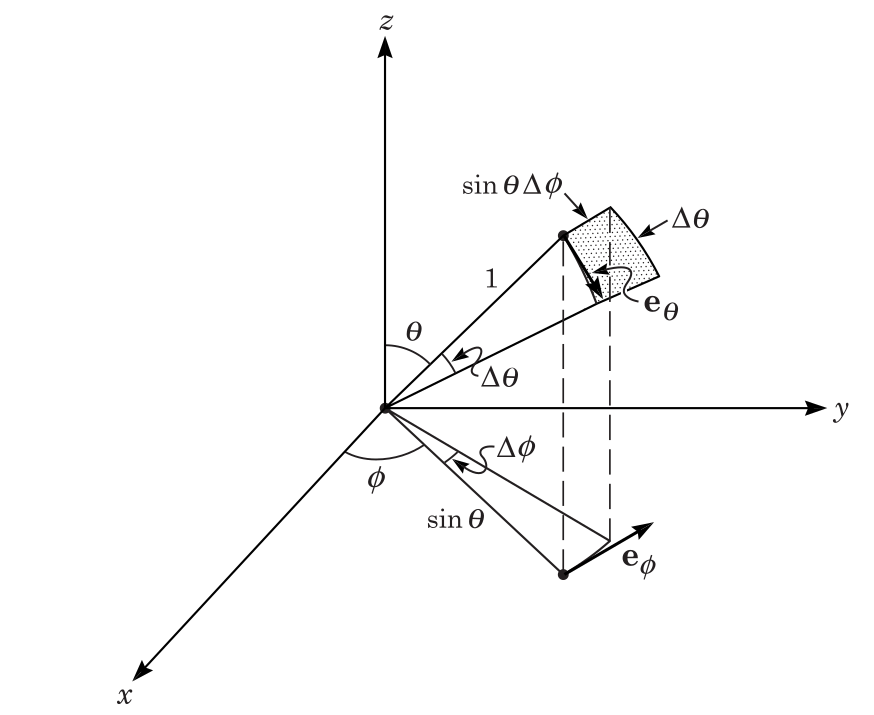
\includegraphics[width=12cm]{Contents/chapter2/figures/7.png}
	\caption{用于描述单位球面上的定向位移$\Delta \bu$的球面极坐标系}
	\label{用于描述单位球面上的定向位移的球面极坐标系}
\end{figure}

为了进一步深入研究, 有必要对蠕虫链的跃迁概率$\Phi(\Delta \bu;\br,\bu)$的形式进行明确说明. 为此, 图\ref{用于描述单位球面上的定向位移的球面极坐标系}所示的球面极坐标系是最方便的. 在单位球面上增大极角$\theta$方向和指向角$\phi$方向上的正交单位矢量分别用$\mathrm{e}_\theta$和$\mathrm{e}_\phi$表示. 对方程(\ref{蠕虫链弯曲能表达式})进行离散后, 单位球沿$\mathrm{e}_\theta$和$\mathrm{e}_\phi$的小位移$\Delta \bu=(\Delta \theta ,\sin \theta \ \Delta \phi)$引起的弯曲能, 即\\
\begin{equation}
\beta\Delta U_0 =\frac{\lambda}{2\Delta s}|\Delta \bu|^2 =\frac{\lambda}{2\Delta s}[(\Delta\theta)^2+(\sin \theta \Delta \phi)^2]
\end{equation}
因此, 跃迁概率$\Phi(\Delta \bu;\br,\bu)\sim 
\exp(-\beta \Delta U_0)$是一个高斯分布, 且有一阶矩和二阶矩\\
\begin{equation}
\langle \Delta \bu\rangle_\Phi =0,\quad \langle \Delta \bu\Delta \bu\rangle_\Phi =\frac{\Delta s}{\lambda}(\mathrm{e}_\theta \mathrm{e}_\theta+\mathrm{e}_\phi \mathrm{e}_\phi)
\end{equation}
将此结果代入方程(\ref{Fokker-Planck方程})将得到所需的Fokker-Planck方程(Hermans和Ullman, 1952)\\
\begin{equation}
	\frac{\partial}{\partial s}p_0(\br,\bu,s) =-\bu \cdot \nabla_{\br} \ p_0(\br,\bu,s)+\frac{1}{2\lambda}\nabla_{\bu}^2\  p_0(\br,\bu,s)\label{简化的Fokker-Planck方程}
\end{equation}
其中$\nabla_{\bu}^2$表示单位球面上的拉普拉斯算子\\
\begin{equation}
\nabla_{\bu}^2 f \equiv \frac{1}{\sin\theta}\frac{\partial}{\partial\theta}\left(\sin\theta \frac{\partial f}{\partial \theta}\right)+\frac{1}{\sin^2\theta}\frac{\partial^2f}{\partial\phi^2}
\end{equation}
这个算子通常被称为旋转扩散算子, 因为它在单位球面上产生扩散运动(Berne和Pecora, 1976). 在方程(\ref{简化的Fokker-Planck方程})中, 参数$1/(2\lambda)$乘以$\nabla_{\bu}^2$可以看作是一个旋转扩散系数. \\

Fokker-Planck 方程(\ref{简化的Fokker-Planck方程})提供了沿蠕虫状聚合物链的关于链段位置和指向传播的完整信息. 这个方程显然没有一个简单的封闭形式的解析解, 尽管它的空间傅里叶变换可以用连续分式展开(Spakowitz和Wang, 2004). 关于数值方法的讨论将推迟到第3.6节. \\

如果我们将注意力限制在指向相关性上, 那么很容易引入第二个约化分布函数\\
\begin{equation}
	H_0(\bu,s)\equiv\int \ p_0(\br,\bu,s)\ d\br\label{第二个约化分布函数}
\end{equation}
它可以解释为一条轮廓长度$s$的蠕虫状链的末端具有指向$\bu$的概率密度. 将$H_0(\bu,s)$归一化, 使得$\int \  H_0(\bu,s)\ d\bu=1$. 在周期边界条件下, 可对方程(\ref{简化的Fokker-Planck方程})在$\br$上积分, 得到约化指向分布函数的Fokker-Planck方程\\
\begin{equation}
	\frac{\partial}{\partial s}H_0(\bu,s)=\frac{1}{2\lambda}\nabla_{\bu}^2\ H_0(\bu,s)\label{约化指向分布函数的Fokker-Planck方程}
\end{equation}
这个方程现在是一个简单的旋转扩散方程, 它具有解析解(Berne和Pecora, 1976;Saito等人, 1967). 为此, 很容易在$H_0(\bu,s)$上引入球谐函数展开, \\
\begin{equation}
	H_0(\bu,s)=\sum_{l=0}^{\infty}\sum_{m=-l}^{l}h_{lm}(s)Y_{lm}(\bu)\label{球谐函数展开}
\end{equation}
其中球谐函数$Y_{lm}(\bu)$是旋转扩散算子的特征函数
\begin{equation}
\nabla_{\bu}^2Y_{lm}(\bu) =-l(l+1)Y_{lm}(\bu)
\end{equation}

这些函数有不同的定义(Edmonds, 1974). 在这里, 我们采用了量子力学中常见的惯例(Schiff, 1968), 并对整数$l,m\geq 0$, 定义$Y_{lm}(\bu)$\\
\begin{equation}
Y_{lm}(\bu) = Y_{lm}(\theta,\phi)=(-1)^m\left[\frac{2l+1}{4\pi}\frac{(l-m)!}{(l+m)!}\right]^{1/2}P_l^m(\cos \theta )\ \exp(im\phi)
\end{equation}
其中$P_l^m(x)$与勒让德函数相关,定义为对整数$l,m\geq 0$, 有\\
\begin{equation}
P_l^m(x)=(1-x^2)^{m/2}\frac{d^m}{dx^m}P_l(x)
\end{equation}
且$P_l(x)$是常见的勒让德多项式, \\
\begin{equation}
P_l(x)=\frac{1}{2^ll!}\frac{d^l}{dx^l}(x^2-1)^l\quad l\geq 0
\end{equation}
对负整数$m$的球谐函数用对称性定义\\
\begin{equation}
Y_{l,-m}(\theta,\phi) =(-1)^m Y_{lm}^*(\theta,\phi)
\end{equation}
星号表示复共轭. 它们在某种意义上是正交的\\
\begin{equation}
\begin{aligned}
\int  \left[Y_{lm}(\bu)\right]^*Y_{l'm'}(\bu)\ d\bu&=\int_{0}^{2\pi}\int_{0}^{\pi}\sin\theta\left[Y_{lm}(\theta,\phi)\right]^*Y_{l'm'}(\theta,\phi) \ d\phi\   d\theta\\&=\delta_{ll'}\delta_{mm'}
\end{aligned}
\end{equation}
并为单位球面上的函数展开构建了一组完全基. \\

将方程(\ref{球谐函数展开})代入方程(\ref{约化指向分布函数的Fokker-Planck方程}), 可写出旋转扩散方程的通解
\begin{equation}
H_0(\bu,s)=\int \ G(\bu,\bu',s)H_0(\bu',0)\ d\bu'
\end{equation}
这个表达式的核心是具有以下球谐函数展开的格林函数:\\
\begin{equation}
G(\bu,\bu',s) = \sum_{l=0}^{\infty}\sum_{m=-l}^{l}\left[Y_{lm}(\bu')\right]^*Y_{lm}(\bu)\exp[-sl(l+1)/(2\lambda)]
\end{equation}
$G(\bu,\bu',s)$描述了轮廓长度$s$的链段具有指向$\bu$的末端和指向$\bu'$的起始端的条件概率. 这个格林函数对于分析理想蠕虫链的统计性质特别有用. 

一些主要感兴趣的是指向相关函数\\
\begin{equation}
	\langle \bu(s)\cdot \bu(s')\rangle =\frac{1}{4\pi}\int \int \bu\cdot \bu'G(\bu,\bu',|s-s'|)\ d\bu d\bu'\label{指向相关函数}
\end{equation}
对于计算这类相关函数, 一个方便的公式是球谐函数加法定理(Edmonds, 1974)\\
\begin{equation}
P_l(\bu\cdot \bu')=\frac{4\pi}{2l+1}\sum_{m=-l}^{l}[Y_{lm}(\bu)]^*Y_{lm}(\bu')
\end{equation}
这个表达式的使用和方程(\ref{指向相关函数})中格林函数的球谐函数展开导致了\\
\begin{equation}
	\langle \bu(s) \cdot \bu(s')\rangle=\exp(-|s-s'|/\lambda)\label{简化的指向相关函数}
\end{equation}
微观长度$λ$的物理解释变得清楚;$λ$是持续长度, 即沿着蠕虫状链的轮廓定向相关衰减的距离. \\

上述结果可用于推导蠕虫链端到端向量的均方. 从表达\\
\begin{equation}
R^2 \equiv\langle|\br(L_c)-\br(0)|^2\rangle =\int_{0}^{L_c} \int_{0}^{L_c}\langle \bu(s)\cdot \bu(s')\rangle\  ds ds'
\end{equation}
插入(\ref{简化的指向相关函数}),我们得到\\
\begin{equation}
	R^2 =2\lambda\{L_c-\lambda[1-\exp(-L_c/\lambda)]\}\label{端到端向量的均方}
\end{equation}
这个表达式是在柔性理想链和刚性杆的性质之间连续插值的. 在柔性极限中, 它对应的轮廓长度远大于持久长度, $L_c/\lambda \gg 1$, 方程(\ref{端到端向量的均方})化简为\\
\begin{equation}
R\approx(2\lambda L_c)^{1/2} \quad (L_c/\lambda \gg 1)
\end{equation}
这与自由连接链的理想链标度公式$R=bN^{1/2} $一致, 如果我们选择将$N=L_c/\lambda$解释为统计独立的持久段数并令$b=\sqrt{2}\lambda$. 相反的极限$L_c/\lambda \ll 1$, 方程(\ref{端到端向量的均方})化简为\\
\begin{equation}
R \approx L_c \quad (L_c/\lambda \ll 1)
\end{equation}
这显然是刚性杆聚合物的精确结果. 因此, 通过改变蠕虫类链模型中的两个参数$\lambda$和$L_c$, 可以描述具有广泛骨架柔性的理想聚合物的统计力学. \\

在讨论完蠕虫链之前, 应该注意到一些作者考虑了模型的变体, 其中$\bu(s)$是一个单位向量这一约束是局部放松的(Freed, 1972;Harris和Hearst, 1966). 在这些变体中, 引入了拉格朗日乘子, 使$\bu(s)$以某种全局平均方式具有单位幅度. 另一种看似更自然的方法(Tagami, 1969;Saito和Namiki, 1956;Yamakawa, 1997)是用调和势$U(\bu)=(3/2)|\bu|^2$代替约束$|\bu(s)=1|$, 并改变方程(\ref{简化的Fokker-Planck方程})右手边的旋转扩散算子, 有\\
\begin{equation}
	\frac{\partial}{\partial s}p_0(\br,\bu,s)=-\bu\cdot \nabla_{\br} \ p_0(\br,\bu,s)+\frac{1}{2\lambda}\nabla_{\bu}\cdot [(\nabla_{\bu}U+\nabla_{\bu})\ p_0(\br,\bu,s)]\label{改变扩散算子后的Fokker-Planck方程}
\end{equation}
在这个方程中, $\bu$不再被限制在单位球面上, 因此相空间$(\br,\bu)$与严格蠕虫链的五维空间相比, 是六维空间. 很容易证明方程(\ref{改变扩散算子后的Fokker-Planck方程})与稳态解$p_0(\br,\bu,\infty)\sim \exp[−U(\bu)]=\exp[−(3/2)|\bu|^2]$是一致的. 因此, 在稳态的情况下, $\langle |\bu|^2\rangle=1$. 这个Fokker-Planck方程与描述带有惯性粒子的布朗运动的方程密切相关, 并且有一个精确的, 尽管复杂的封闭形式的解(Chan-drasekhar, 1943). 由于当我们考虑外部势中链的更真实的情况(第三章的主题)时, 这个优势就失去了, 因此在高维相空间中工作所增加的计算负担使得模型不像真正的蠕虫链那么理想. \\

最后, 值得注意的是, 蠕虫链模型已被很好地扩展去描述螺旋线形成的趋势(Yamakawa, 1997). 这一扩展对于建立与蛋白质和其他生物分子有关的统计力学模型具有重要意义. 这些生物分子能够在溶液中形成二级结构. \\
\endinput



\chapter{外场中的单链配分函数}
\section{外场中的单链}
{\color{red}\begin{center}
        刘江刚
    \end{center}}

在前一章中,我们描述了理想链统计力学的各种模型。在这里,这些模型被推广到包括一个或多个作用于聚合物链的各个部分的势场。在本章中,额外的场将被视为“外部”,因为它们可以任意指定。然而,我们将在第4章中看到,最重要的势场是那些由周围聚合物段的力场自洽产生的场。

由于这一主题对非均匀聚合物理论的重要性,本章中的论述是相当详细的,精确评价单个聚合物在指定势场中的统计力学是基于场的计算机模拟中计算量最大的部分,也是成功的分析理论的重要组成部分。

\section{配分函数和分布函数}
我们的第一项任务是讨论理想链模型的配分函数和分布函数是如何在外场存在的情况下改变的。我们从离散高斯链开始。
\subsection{离散高斯链}
我们主要感兴趣的外场是一个空间变化的化学势场$w(\br)$,它作用于离散高斯链的$N+1$个珠子上,我们再次采用图2.1和2.3节的记号。势能可以写成
\begin{equation}\label{3.1}
\begin{aligned}
U(\br^{N+1})&=U_0(\br^{N+1})+U_1(\br^{N+1})\\
&=\sum\limits_{i=1}^Nh(\left|\br_i-\br_{i-1}\right|)+k_BT\sum\limits_{i=0}^Nw(\br_i)
\end{aligned}
\end{equation}
这里$h(x)=3k_BTx^2/(2b^2)$和$\br^{N+1}$是$N+1$个珠子坐标$(\br_0,\br_1,\cdots,\br_N)$的缩写。$N$键上的第一个和是$U_0$,这是离散高斯链的谐波拉伸能(harmonic stretching energy)。$N+1$个珠子上的第二个和计算了每个珠子与势场$k_BTw(\br)$的相互作用能。另一种表示外部势能项$U_1(\br^{N+1})$的方法是
\begin{equation}\label{3.2}
\beta U_1(\br^{N+1})=\int~w(\br)\hat{\rho}(\br)\mathrm{d}\br
\end{equation}
其中段的微观密度由下式子定义:
\begin{equation}\label{3.3}
\hat{\rho}(\br)=\sum\limits_{i=0}^N\delta(\br-\br_i)
\end{equation}
这种微观密度显然是$\br$的非常奇异的函数,并且显然地依赖于珠子坐标$\br^{N+1}$。式子(\ref{3.2})表示的事实是,势场$w(\br)$可以看作是一个空间变化的化学势场,它是热力学共轭于段密度的化学势场(Chandler,1987)。

特别令人感兴趣的是,受外部势场$w(\br)$作用的链的配分函数$Z[w]$与理想链的配分函数$Z_0$的比率。
\begin{equation}\label{3.4}
Q(w)\equiv\frac{Z[w]}{Z_0}=\frac{\int\exp[-\beta U(\br^{N+1})]\mathrm{d}\br^{N+1}}{V(\int\exp[-\beta h(\left|\bb\right|)]\mathrm{d}\bb)^N}
\end{equation}
在该表达式的分母中,使用了方程(\ref{2.32}),它将$Z_0$表示为键向量上的体积$V$乘以$N$个独立(体积)积分,如记号所示,归一化配分函数$Q[w]$可以看作是外部势场$w(\br)$的泛函。

下一步是将方程(\ref{3.4})的分母中的$\int\mathrm{d}\bb~\exp[-\beta h(\left|\bb\right|)]$的$N$个因子与分子中的$\exp[-\beta h(\left|\br_i-\br_{i-1}\right|)]$的$N$个因子相关联。回顾离散高斯链的归一化键转移概率的定义,方程(\ref{2.39})
\begin{equation}\label{3.5}
\Phi(\br)=\frac{\exp[-\beta h(\left|\br\right|)]}{\int\exp[-\beta h(\left|\br\right|)]\mathrm{d}\br}=\left(\frac{3}{2\pi b^2}\right)^{3/2}~\exp\left(-\frac{3\left|\br\right|^2}{2b^2}\right)
\end{equation}
使方程(\ref{3.4})重写为
\begin{equation}\label{3.6}
\begin{aligned}
Q[w]=\frac{1}{V}\int&[e^{-w(\br_N)}\Phi(\br_N-\br_{N-1})e^{-w(\br_{N-1})}\Phi(\br_{N-1}-\br_{N-2})\\
&\cdots e^{-w(\br_2)}\Phi(\br_2-\br_1)e^{-w(\br_1)}\Phi(\br_1-\br_0)e^{-w(\br_0)}]\mathrm{d}\br^{N+1}
\end{aligned}
\end{equation}
这个表达式可以按以下方式递归重写。我们对整数$j$定义了一个泛函$q(\br,j;[w])$通过
\begin{equation}\label{3.7}
q(\br,0;[w])=\exp[-w(\br)]
\end{equation}
和对$j=0,1,2,\cdots,N-1$
\begin{equation}\label{3.8}
q(\br,j+1;[w])=\exp[-w(\br)]\int\Phi(\br-\br')q(\br',j;[w]))\mathrm{d}\br'
\end{equation}
因此,归一化的配分函数可以表示为
\begin{equation}\label{3.9}
Q[w]=\frac{1}{V}\int~q(\mathrm{r},N;[w])\mathrm{d}\br
\end{equation}
在上文中,$q(\br,j;[w])$表示$j+1$个珠子链在$r$位置处的统计权重。该对象通常被称为链传播子,是外部势场$w(\br)$的泛函。方程(\ref{3.8})可以看作是一个Chapman-Kolmogorov方程,对于无场情况下概率密度$p_0(\mathrm{r},j)$,它与式子(\ref{2.38})严格类似。实际上,除了函数$p_0(\br,j)$和$q(\br,j;[w])$的不同归一化之外,方程(\ref{3.8})当$w(\mathrm{r})\rightarrow 0$时简化为方程(\ref{2.38})。

需要注意的是,对于任何弹簧势$h(x)$,方程(\ref{3.7})-(\ref{3.9})都是成立的,条件是用适当的形式代替高斯模型方程(\ref{3.5})的转移概率密度$\Phi(\br)$。参见方程(\ref{2.45}),方程(\ref{3.7})-(\ref{3.9})适用于方程(\ref{2.46})等非线性珠弹簧模型。
\begin{figure}[H]
\centering
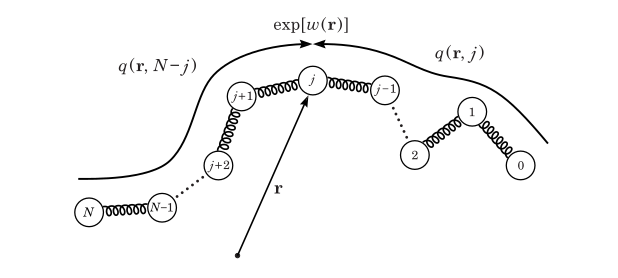
\includegraphics[scale=0.7]{Contents/chapter3/figures/Figure_1.png}
\caption{因式分解性质方程(\ref{3.10})的物理内容,具有$j+1$个珠的传播子可以在第$j$个珠的位置$\br=\br_j$处连接到具有$N-j+1$个珠的传播子,以产生链的总统计量。在结点处需要$\exp[w(\br)]$的因子。}
\end{figure}
归一化配分函数$Q[w]$具有一个重要的因式分解性质,如图3.1所示。如果我们选择在珠$j$处计算方程(\ref{3.6}),那么很明显,$Q[w]$是可以成
\begin{equation}\label{3.10}
Q[w]=\frac{1}{V}\int~q(\br,N-j;[w])~\exp[w(\br)]q(\br,j;[w])\mathrm{d}\br
\end{equation}
这个表达式的物理解释是,$(N+1)$珠链的统计权重可以通过连接用于$j+1$珠子的末端分布的传播子和用于“互补”链的$N-j+1$珠子的传播子来建立。传播子在第$j$个珠的位置$\br=\br_j$连接,并包含$\exp[w(\br)]$以抵消与两个连接端相关联的$\exp[-w(\br)]$多余因子。

第二类外势对研究聚合物的力学效应具有重要意义,它是一个应变场。在这里,我们限制了对均匀应变$\boldsymbol{\epsilon}(\br)=\boldsymbol{\epsilon}$的关注,以了解这种对称张量场是如何与聚合物的统计力学耦合的,需要注意的是,可以写出离散高斯链弹性应力张量(elastic stress tensor)的微观表达式(Doi和Edwards,1986)为
\begin{equation}\label{3.11}
\hat{\sigma}_{\alpha\gamma}(\br)=\frac{3k_BT}{b^2}\sum\limits_{i=1}^N\delta(\br-\br_{i-1})(\br_{i}-\br_{i-1})_{\alpha}(\br_i-\br_{i-1})_{\gamma}
\end{equation}
其中希腊语下标用于表示张量的笛卡尔指数,该表达式将与穿过规定平面的聚合物键相关的每单位面积弹力相加。利用应力和应变是共轭热力学变量的事实,(Landau和Lifshitz,1986),可以写出与施加的应变$\epsilon$相关的弹性能量。
\begin{equation}\label{3.12}
U_{el}(\br^{N+1})=\int\boldsymbol{\epsilon}:\hat{\boldsymbol{\sigma}}(\br)\mathrm{d}\br
\end{equation}
特别令人感兴趣的是一个受化学势场和应变场双重作用的离散高斯链的配分函数$Z[w,\epsilon]$。在这种情况下,最方便的归一化是$w=0$的链的配分函数,但不消失应变
\begin{equation}\label{3.13}
Q[w,\boldsymbol{\epsilon}]\equiv\frac{Z[w,\boldsymbol{\epsilon}]}{Z[0,\boldsymbol{\epsilon}]}=\frac{\int\exp[-\beta U(\br^{N+1})-\beta U_{el}(\br^{N+1})]\mathrm{d}\br^{N+1}}{\int\exp[-\beta U_0(\br^{N+1})-\beta U_{el}(\br^{N+1})]\mathrm{d}\br^{N+1}}
\end{equation}
使得方程(\ref{3.7})-(\ref{3.9})仍然成立,但随着键转移概率的变化
\begin{equation}\label{3.14}
\Psi(\br;[\boldsymbol{\epsilon}])=\left(\frac{3}{2\pi b^2}\right)^{3/2}[det(\boldsymbol{1}+2\boldsymbol{\epsilon})]^{1/2}\exp\left(-\frac{3}{2b^2}(1+2\boldsymbol{\epsilon}:\br~\br)\right)
\end{equation}
其中$\boldsymbol{1}$表示单位张量。在推导这个表达式时使用了方程(B.11),在无应变情况下,$Q[w,\epsilon]$可以根据
\begin{equation}\label{3.15}
Q[w,\boldsymbol{\epsilon}]=\frac{1}{V}\int~q(\br,N;[w,\boldsymbol{\epsilon}])\mathrm{d}\br
\end{equation}
计算且
\begin{equation}\label{3.16}
q(\br,0;[w,\boldsymbol{\epsilon}])=\exp[-w(\br)]
\end{equation}
和
\begin{equation}\label{3.17}
q(\br,j+1;[w,\boldsymbol{\epsilon}])=\exp[-w(\br)]\int\Psi(\br-\br';[\boldsymbol{\epsilon}])~q(\br',j;[w,\boldsymbol{\epsilon}])\mathrm{d}\br'
\end{equation}
对于$j=0,1,2,\cdots,N-1$。这些方程在消失应变$\boldsymbol{\epsilon}\rightarrow 0$的极限下明显简化到方程(\ref{3.7})-(\ref{3.9}),在消失应变和化学势$\boldsymbol{\epsilon},w\rightarrow 0$的极限下简化为方程(\ref{2.38})。
\subsection{连续高斯链}
前一段的公式可以很容易地推广到连续高斯链模型,微观段密度由方程(\ref{3.3})变为
\begin{equation}\label{3.18}
\hat{\rho}(\br)=\int_0^N\delta(\br-\br(s))\mathrm{d}s
\end{equation}
与施加的化学势场$w(\br)$相关的势能成为聚合物形状$\br(s)$的泛函。
\begin{equation}\label{3.19}
\beta U_1[\br,w]=\int~w(\br')\hat{\rho}(\br')\mathrm{d}\br'
\end{equation}
归一化配分函数$Q[w]$可以表示为路径积分的比率。
\begin{equation}\label{3.20}
Q[w]\equiv\frac{Z[w]}{Z_0}=\frac{\int\exp(-\beta U_0[\br]-\beta U_1[\br,w])\calD\br}{\int\exp(-\beta U_0[\br])\calD\br}
\end{equation}
在此定义下,$Z_0$的奇点从分子和分母中完全消失,在连续链极限情况下$Q[w]$有限。利用$N_s+1$珠和$N_s$弹簧,根据方程(\ref{2.50})对两个路径积分进行离散化,并对离散高斯链得到方程(\ref{3.6})的步骤进行了回溯。因此,方程(\ref{3.20})减少到
\begin{equation}\label{3.21}
\begin{aligned}
Q[w]=\frac{1}{V}&\int[e^{-\Delta sw(\br_{N_s})}\Phi(\br_{N_s}-\br_{N_s-1})e^{-\Delta sw(\br_{N_s-1})}\\
&\times\quad\Phi(\br_{N_s-1}-\br_{N_s-2})\cdots e^{-\Delta sw(\br_2)}\\
&\times\quad\Phi(\br_2-\br_1)e^{-\Delta sw(\br_1)}\Phi(\br_1-\br_0)e^{-\Delta sw(\br_0)}]\mathrm{d}\br^{N_s+1}
\end{aligned}
\end{equation}
其中$\Phi(\br-\br')=\Phi(\Delta\br)$由方程(\ref{2.64})给出和$\Delta s\equiv N/N_s$。和以前一样,$Q[w]$的表达式可以写成
\begin{equation}\label{3.22}
Q[w]=\frac{1}{V}\int~q(\br,N;[w])\mathrm{d}\br
\end{equation}
这里
\begin{equation}\label{3.23}
q(\br,0;[w])=\exp[-\Delta sw(\br)]
\end{equation}
和
\begin{equation}\label{3.24}
q(\br,s+\Delta s;[w])=\exp[-\Delta s~w(\br)]\int\Phi(\br-\br')q(\br',s;[w])\mathrm{d}\br'
\end{equation}
在$N_s$中以$\Delta s$为增量沿着从$s=0$到$s=N$链的方向。

方程(\ref{3.24})是一个Chapman-Kolmogorov方程,与无场情况下的方程(\ref{2.63})密切相关,它可以在$\Delta s\rightarrow 0$的连续极限情况下转化为Fokker-Planck方程。利用泰勒展式在$\Delta s$处将方程(\ref{3.24})的两边展开为一阶的,在$\Delta\br=\br-\br'$处将被积函数展开为二阶的,人们发现(Edwards,1965;de Gennes,1969;Freed,1972)
\begin{equation}\label{3.25}
\frac{\partial}{\partial s}q(\br,s;[w])=\frac{b^2}{6}\nabla^2q(\br,s;[w])-w(\br)q(\br,s;[w])
\end{equation}
它可以看作是方程(\ref{2.69})在包括外部势场情况下的推广。“初始条件”方程(\ref{3.23})在连续极限下简化到均匀条件。
\begin{equation}\label{3.26}
q(\br,0;[w])=1
\end{equation}
Fokker-Planck方程(\ref{3.25})通常称为修正的扩散方程,有时与量子力学的路径积分公式相似,称为Feynman-Kac公式(Feynman和Hibbs,1965)。结合方程(\ref{3.22}),修正的扩散方程充分描述了外部势场$w(\br)$中连续高斯链的统计力学。这是非均匀聚合物理论中最重要的结果之一。

势场$w(\br)$中的连续高斯链具有类似于离散高斯链方程(\ref{3.10})的因式分解性质。特别是,
\begin{equation}\label{3.27}
Q[w]=\frac{1}{V}\int~q(\br,N-s;[w])q(\br,s;[w])\mathrm{d}\br
\end{equation}
其中路径积分已被分解为$0<s<N$任意轮廓位置。由于连续极限在$\Delta s\rightarrow 0$时$\exp[\Delta sw(\br)]\rightarrow 1$,因此在连接端消除多余的因子$\exp[-\Delta sw(\br)]$所需的指数因子$\exp[\Delta sw(\mathrm{r})]$是不存在的。

除了化学势场$w(\br)$外,这些结果很容易推广到均匀应变场$\boldsymbol{\epsilon}$作用下的连续高斯链情形。将微观弹性应力表达式(\ref{3.11})修正为连续高斯链
\begin{equation}\label{3.28}
\hat{\sigma}_{\alpha\gamma}(\br)=\frac{3k_BT}{b^2}\int_0^N\delta(\br-\br(s))\mathrm{d}s\frac{\mathrm{d}\br_{\alpha}(s)}{\mathrm{d}s}\frac{\mathrm{d}\br_{\gamma}(s)}{\mathrm{d}s}
\end{equation}
弹性能可以表示为$\br(s)$和$\boldsymbol{\epsilon}$的泛函
\begin{equation}\label{3.29}
U_{el}[\br,\boldsymbol{\epsilon}]=\int\boldsymbol{\epsilon}:\hat{\boldsymbol{\sigma}}(\br')\mathrm{d}\br'
\end{equation}
对于受应变和化学势场的连续链的归一化配分函数是
\begin{equation}\label{3.30}
Q[w,\boldsymbol{\epsilon}]\equiv\frac{Z[w,\boldsymbol{\epsilon}]}{Z[0,\boldsymbol{\epsilon}]}=\frac{\int\exp(-\beta U_0[\br]-\beta U_1[\br,w]-\beta U_{el}[\br,\boldsymbol{\epsilon}])\calD\br}{\int\exp(-\beta U_0[\br]-\beta U_{el}[\br,\boldsymbol{\epsilon}])\calD\br}
\end{equation}
再次,归一化是$Q[0,\boldsymbol{\epsilon}]=1$,根据方程(\ref{2.50})离散分子和分母中的路径积分并且回溯推导方程(\ref{3.25})的步骤产生以下结果(Fredrickson,2002)
\begin{equation}\label{3.31}
Q[w,\boldsymbol{\epsilon}]=\frac{1}{V}\int~q(\br,N;[w,\boldsymbol{\epsilon}])\mathrm{d}\br
\end{equation}
其中传播子$q(\br,s;[w,\boldsymbol{\epsilon}])$满足Fokker-Planck方程。
\begin{equation}\label{3.32}
\begin{aligned}
\frac{\partial}{\partial s}q(\br,s;[w,\boldsymbol{\epsilon}])=&-w(\br)~q(\br,s;[w,\boldsymbol{\epsilon}])\\
&+\frac{b^2}{6}(1+2\boldsymbol{\epsilon})^{-1}:\nabla\nabla~q(\br,s;[w,\boldsymbol{\epsilon}])
\end{aligned}
\end{equation}
这个方程受初始条件的影响。
\begin{equation}\label{3.33}
q(\br,0;[w,\boldsymbol{\epsilon}])=1
\end{equation}
Fokker-Planck方程(\ref{3.32})在消失应变情况下可简化为方程(\ref{3.25})。然而,在$\boldsymbol{\epsilon}$有限的条件下,它描述了一个各向异性扩散过程,它与同时经历化学势场和应变场的聚合物链相一致。这些结果可进一步推广到非均匀应变场$\boldsymbol{\epsilon}(\br)$的情形(Fredrickson,2002)。
\subsection{蠕虫状链}
蠕虫状链模型也可以类似地推广到包含外场作用的情况下。与高斯链模型不同的是,蠕虫状链通常用来描述具有局部刚性的聚合物,其能够呈现液晶的有序性。这种液晶在微观水平上来自各向异性的链段相互作用。因此,重要的是允许当前情况下的外部“化学”势既取决于链段位置,也取决于链段方向,即$w=w(\br,\bu)$。蠕虫状链与这样一个场的相互作用能可以写成。
\begin{equation}\label{3.34}
\begin{aligned}
\beta U_1[\br,w]&=\int_0^{L_c}w(\br(s),\bu(s))\mathrm{d}s\\
&=\int\mathrm{d}\br'\int~w(\br',\bu')\hat{\rho}(\br',\bu')\mathrm{d}\bu'
\end{aligned}
\end{equation}
这里
\begin{equation}\label{3.35}
\hat{\rho}(\br,\bu)\equiv\int_0^{L_c}\delta(\br-\br(s))\delta(\bu-\bu(s))\mathrm{d}s
\end{equation}
是片段位置和取向的微观位置。势场$w(\br,\bu)$与这个密度是热力学共轭的。

在无势场$Z_0$的情况下,用它的值归一化具有势场$w(\br,\bu)$蠕虫链的配分函数$Z[w]$
\begin{equation}\label{3.36}
Q[w]\equiv\frac{Z[w]}{Z_0}=\frac{\int^*\exp(-\beta U_0[\bu]-\beta U_1[\br,w])\calD\br}{\int^*\exp(-\beta U_0[\mathrm{u}])\calD\br}
\end{equation}
其中$U_0[\mathrm{u}]$是方程(\ref{2.71})中给出的弯曲能。分子和分母中路径积分上的星号是表示方程(\ref{2.72})的约束的简记,即
\begin{equation}\label{3.37}
\prod\limits_s\delta\left(\bu(s)-\frac{\mathrm{d}\br(s)}{\mathrm{d}s}\right)\delta(\left|\bu(s)\right|-1)
\end{equation}
是强加于链构相$\br(s)$上的。

方程(\ref{3.36})可以通过离散分子和分母中的路径积分和类似于(\ref{2.76})推导链传播子$q(\br,\bu,s;[w])$的Chapman-Kolmogorov方程来推导。这个量描述了轮廓长度为$s$的蠕虫状链的统计权重,并且位于势场$w(\br,\bu)$,其末端段位于位置$\br$并且具有方向$\bu$。归一化配分函数是
\begin{equation}\label{3.38}
Q[w]=\frac{1}{4\pi V}\int\mathrm{d}\br\int~q(\br,\bu,L_c;[w])\mathrm{d}\bu
\end{equation}
在连续极限的情况下,我们发现蠕虫状链传播子$q(\br,\bu,s;[w])$满足无场情况下类似方程(\ref{2.81})的Fokker-Planck方程:
\begin{equation}\label{3.39}
\begin{aligned}
\frac{\partial}{\partial s}q(\br,\bu,s;[w])=&-w(\br,\bu)~q(\br,\bu,s;[w])-\bu\cdot\nabla_{\br}~q(\br,\bu,s;[w])\\
&+\frac{1}{2\lambda}\nabla_{\bu}^2~q(\br,\bu,s;[w])
\end{aligned}
\end{equation}
这个方程是在下面初始条件下求解的
\begin{equation}\label{3.40}
q(\br,\bu,0;[w])=1
\end{equation}
方程(\ref{3.38})-(\ref{3.40})是定义具有外部势场的蠕虫状链的统计力学的基本关系。

蠕虫状链的归一化配分函数具有类似于连续高斯链的因式分解性质。从$Q[w]$的离散表达式可以直接推断出
\begin{equation}\label{3.41}
Q[w]=\frac{1}{4\pi V}\int\mathrm{d}\br\int~q(\br,-\bu,L_c-s;[w])q(\br,\bu,s;[w])\mathrm{d}\bu
\end{equation}
对于任意$0\le s\le L$。在物理上,这个公式表明,对于总轮廓长度$L_c$的聚合物的配分函数可以通过组成用于轮廓长度$s$的链段的传播子与用于长度为$L_c-s$的链的第二传播子来建立。与第一传播子$q(\br,\bu,s;[w])$相关的统计权重是通过从聚合物的$s=0$段开始在方程(\ref{3.39})-(\ref{3.40})沿$s$方向积分得到的。第二个传播子$q(\br,-\bu,L_c-s;[w])$对应于通过求解方程(\ref{3.39})-(\ref{3.40})得到的长度为$L_c-s$的链的统计权重,从另一端开始的聚合物。该权重中的切向量$u$在符号中是反向的,以说明沿链轮廓的传播方向的差异。

虽然我们把$w$称为外化学势场,但所采用的形式$w=w(\br,\bu)$足以描述多种类型的外势,包括电场和磁场。例如,一种感兴趣的情况是沿着主干具有永久电偶极子的链,它与切线向量$\bu(s)$共线,即$\mu(s)=\mu_0\bu(s)$。在这种情况下,与施加的静止电场$\bE(\br)$相关的静电能由方程(\ref{3.34})给出
\begin{equation}\label{3.42}
w(\br,\bu)=-\beta\mu_0\bE(\br)\cdot\bu
\end{equation}
作为另一个例子,在静电场$\bE(\br)$作用下,介电蠕虫状链可以用下面势来描述:
\begin{equation}\label{3.43}
w(\br,\bu)=-\frac{\beta}{2}\bE(\br)\cdot\boldsymbol{\alpha}(\bu)\cdot\bE(\br)
\end{equation}
其中$\boldsymbol{\alpha}(\bu)$是取向$\bu$的差分链段的极化率张量。在关于$\bu$的极化率张量的圆柱对称的特殊情况下,$\boldsymbol{\alpha}(\bu)$可以表示为
\begin{equation}\label{3.44}
\boldsymbol{\alpha}(\bu)=\alpha_{\parallel}\bu\bu+\alpha_{\perp}(1-\bu\bu)
\end{equation}
其中,$\alpha_{\parallel}$和$\alpha_{\perp}$分别是差分链段平行和垂直于切线向量$\bu$的极化率。

类似的表达式可以用来描述蠕虫状链与一大类静态和时变外场之间的相互作用。我们将对液晶的各向异性势场的讨论推迟到4.6节。

不幸的是,沿着蠕虫状链弯曲的三体特性使微观张力的识别变得复杂。在克服这一困难之前,不可能探索蠕虫状链对空间变化应变场的平衡效应。
\subsection{棒状聚合物}
蠕虫状链模型具有一种吸引人的特性,即它根据持续长度和轮廓长度的比值$(\lambda/L_c)$,在刚性杆和柔性线圈之间进行连续插值。因此,它可以用来描述任意主干灵活性的大分子。然而,该模型的一个严重缺点是,在计算热力学和结构量时,需要一个传播子$q(\br,\bu,s)$,它在高斯链模型中传播子$q(\br,s)$之外还有两个附加的内部坐标(定义$\bu$的角度)。在3.6节中,很明显,这些额外的坐标大大增加了用蠕虫状链模型进行数值计算的费用。因此,对于近柔性聚合物$\lambda/L_c\ll 1$,最好用连续高斯链或珠弹簧链模型代替蠕虫状链。类似地,对于接近刚性的棒状聚合物,$\lambda/L_c\gtrsim 1$,采用严格的棒状聚合物模型代替蠕虫状链。对于末端为$\br$且取向为$\bu$的长$L_c$的杆,给出了归一化配分函数如下:
\begin{equation}\label{3.45}
Q[w]=\frac{1}{4\pi V}\int\mathrm{d}\br\int\exp\left[-\int_0^{L_c}\mathrm{d}sw(\br+s\bu,\bu)\right]\mathrm{d}\bu
\end{equation}
给定一定的势场$w(\br,\bu)$,方程(\ref{3.45})显然比蠕虫状链相应的方程(\ref{3.38})-(\ref{3.40})更直观。











































































































\section{单链平均和算子}
{\color{red}\begin{center}
        何志娟
    \end{center}}

在前面的章节中,我们描述了如何使用Chapman-Kolmogorov或Fokker-Planck方程计算单链在外场存在下的分布函数。单链配分函数和约化分布函数(链传播子)是非均匀聚合物理论中的中心对象,有必要将其它“可观测”量表示为外场变量的显式泛函。这主要的量与单链自由度构象全体平均受到外势有关。例如:离散高斯链受到化学势$w (\br)$的情况下,我们可以定义任何函数$f(\br^{N+1})$珠坐标(bead coordinates)的单链平均:
\begin{equation}\label{3.46}
<f(\br^{N+1})>_{[w]}= \frac{\int  f(\br^{N+1})~\exp[-\beta U(\br^{N+1})]~d \br^{N+1}}{\int \exp[-\beta U(\br^{N+1})]~d\br^{N+1}}
\end{equation}

其中$U(\br^{N+1})$是公式(\ref{3.1})给出的电势。尖括号的下标$[w]$在对珠坐标进行平均,平均量可以看作是外场$w(\br)$的函数。同样,对于存在化学势和应变场$w(\br)$和$\mathbf{\epsilon}$的连续高斯链,相应的单链平均值可以定义为:
\begin{equation}\label{3.47}
<f[\br]>_{[w ,\epsilon]}=\frac{\int f[\br]~\exp(-\beta U_{0}[\br]-\beta U_{1}[\br,w]-\beta U_{el}[\br,\epsilon])~D\br}{\int \exp(-\beta U_{0}[\br]-\beta U_{1}[\br,w]-\beta U_{el}[\br,\epsilon])~D\br}
\end{equation}
其中$f[\br]$是链构型$\br(s)$的任意泛函。

主要有趣的单链平均量是段密度、密度相关性和弹性应力,所有这些都可以与非均匀聚合物实验中的可观测值联系起来。我们将看到在某些情况,可以通过取关于场变量$w(\br)$和$\mathbf{\epsilon}$的规范配分函数$Q[w]$和$Q[w,\epsilon]$的函数导数来获得这些结果。读者不熟悉函数的变分,建议参考附录C。
\subsection{密度算子}
首先,我们考虑在化学势$w(\br)$作用下的单个柔性聚合物的平均段数密度的计算问题。这个数量定义为:
\begin{equation}\label{3.48}
\rho(\br;[w])\equiv<\hat{\rho}(\br)>_{[w]}
\end{equation}

其中微观密度$\hat{\rho}(\br)$由公式(\ref{3.3})或(\ref{3.18})给出,这取决于采用的是离散的或连续的高斯链模型。我们将$\rho(\br;[w])$称为单链密度算子,因为它将平均段密度表示为强加场$w$的一个泛函。我们将在第四章中看到,场构造分布合适时,许多聚合物相互作用流体的平均单体密度与算子$\rho(\br;[w])$的平均值成正比。在这种情况下场不是外部强加的,而是由非键单体之间的相互作用在内部产生的。因此,在多链流体中的“可观测”量的计算将涉及两种不同类型全体平均:(i)公式(\ref{3.46})和(\ref{3.47})描述单链的平均;(ii)内部产生电势场分布的场论平均值。关于第二类平均的讨论将推迟到第四章。

在计算公式(\ref{3.48})时,我们再次指出$w(\br)$和$\hat{\rho}(\br)$是热力学共轭变量。因此,$-lnQ[w]$泛函关于$w(\br)$的导数会生成单链$\hat{\rho}(\br)$的平均。例如:在离散高斯链的情况下,关于$Q$的公式(\ref{3.4})和单链平均定义(\ref{3.46})。特别是:
\begin{equation}\label{3.49}
-\frac{\delta~lnQ[w]}{\delta w(\br)}=-\frac{1}{Q[w]}\frac{\delta Q[w]}{\delta w(\br)}=<\hat{\rho}(\br)>_{[w]}
\end{equation}
因此,段密度算子的另一个表达式是
\begin{equation}\label{3.50}
\rho(\br;[w])=-\frac{1}{Q[w]}\frac{\delta Q[w]}{\delta w(\br)}
\end{equation}

这个表达式的右边可以通过公式(\ref{3.6})的泛函微分直接计算(对于离散的高斯链)。这导致:
\begin{equation}\label{3.51}
\begin{aligned}
\frac{\delta Q[w]}{\delta w(\br)}=\frac{1}{V}\sum_{j=0}^{N}\int &[e^{-w(\br_{N})}\Phi(\br_{N}-\br_{N-1})e^{-w(\br_{N-1})}\Phi(\br_{N-1}-\br_{N-2}) \\ &\times \ldots e^{-w(\br_{j})}(-1)\delta(\br-\br_j)\Phi(\br_j-\br_{j-1})e^{-w(\br_j-1)}\\ & \times \ldots e^{-w(\br_{2})}\Phi(\br_{2}-\br_{1})e^{-w(\br_{1})}\Phi(\br_{1}-\br_{0})e^{-w(\br_{0})}]~d \br^{N+1}
\end{aligned}
\end{equation}
公式(\ref{3.51})中的δ函数可以用来消去$\br_{j}$上的积分,即珠 j的位置。这产生了表因式分解的表达示,类似于公式(\ref{3.10})描述的的因式分解性质,如图3.1所示。按照同样的推理,可以通过组成传播子$q(\br,j;[w])$重写公式(\ref{3.51}),用“互补”传播子$q(\br,N-j;[w])$描述链段的统计权重,该链段从珠0开始,终止于珠j。后者描述的统计权重与剩余链段相关,从珠N开始,用珠j完成。因此,公式(\ref{3.51})可以表示为:
\begin{equation}\label{3.52}
\frac{\delta Q[w]}{\delta w(\br)}=-\frac{e^{w(\br)}}{V}\sum_{j=0}^{N}~q(\br,N-j;[w])~q(\br,j;[w])
\end{equation}
因此:	
\begin{equation}\label{3.53}
\rho(\br,[w])=\frac{e^{w}}{VQ[w]}\sum_{j=0}^{N}~q(\br,N-j;[w])~q(\br,j;[w])
\end{equation}

方程(\ref{3.53})是非均匀聚合物理论中的一个重要公式,因为它提供了计算具有任意电势$w(\br)$的离散高斯链平均段密度的方法。给出$w(\br)$的表达式,首先递归求解公式(\ref{3.8})[在初始条件(\ref{3.7})下],得到j=0,1,2,…,N的$q(\br,j;[w])$。其次,用公式(\ref{3.9})计算$Q[w]$。这些结果可用于计算公式(\ref{3.53})右侧的表达式。因此,对所有珠子j的链传播子$q(\br,j;[w])$的知识足以确定规范化配分函数$Q[w]$和平均段密度$\rho(\br;[w])$。

这些结果很容易推广到其他链模型中。按照公式(\ref{3.21})离散的连续高斯链,连续高斯链类似公式(\ref{3.53})的模拟量是:
\begin{equation}\label{3.54}
\begin{aligned}
\rho(\br,[w])&=-\frac{1}{Q[w]}\frac{\delta Q[w]}{\delta w(\br)}\\ &=\frac{\triangle s ~\exp[\triangle sw(\br)]}{VQ[w]}\sum_{j=0}^{N_s}~q(\br,(N_s-j)\triangle s;[w])~q(\br,j\triangle s;[w])
\end{aligned}
\end{equation}
当取连续极限$N_s\to \infty$,$\triangle s=N/N_s\to 0$,时,我们发现这个表达式可以化简为:
\begin{equation}\label{3.55}
\rho(\br,[w])=\frac{1}{VQ[w}\int_{0}^{N}q(\br,(N-s);[w])~q(\br,s;[w])~ds
\end{equation}
这是一个众所周知的结果,是非均匀聚合物的核心理论。其次,我们发现它和连续高斯链(\ref{3.27})的因式分解性质相似。

密度算子$\rho(\br,[w])$描述了链段的平均密度,而不是它们沿聚合物的位置。另一个有用的密度算子,例如:连续高斯链是数量:
\begin{equation}\label{3.56}
\rho(\br,s;[w])\equiv <\hat{\rho}(\br,s)>_{[w]}
\end{equation}
表示位于等高线位置s的分段的平均密度。用$\hat{\rho}(\br,s)=\delta(\br-\br(s))$表示各段在位置s的微观密度。通过引入共轭场$\omega_s(\br)$来计算$\hat{\rho}(\br,s)$
,仅能计算单体s,并对相互作用能贡献一个附加项:
\begin{equation}\label{3.57}
\beta U_1[\br,w ,w_s]=\int [\hat{\rho}(\br^{'})w (\br^{'})+\hat{\rho}(\br^{'},s)w_s(\br^{'})]~d\br^{'}
\end{equation}
下面的参数类似于公式(\ref{3.50})的参数,给出结果:
\begin{equation}\label{3.58}
\rho(\br,s;[w])=<\hat{\rho}(\br,s)>_{[w]}
=-\frac{\delta~lnQ[w,w_s]}{\delta w_s(\br)} \bigg |_{w_s=0}
\end{equation}
我们现回到$Q[w,w_s]$的路径积分离散化的步骤,对$w_s$微分,并取连续极限。如果令$w_s(\br)=0$,结果是:
\begin{equation}\label{3.59}
\rho(\br,s;[w])=\frac{1}{VQ[w]}~q(\br,(N-s);[w])~q(\br,s;[w])
\end{equation}

图\ref{figure1}描述了公式(\ref{3.59})的物理含量,与公式(\ref{3.55})的比较,我们发现平均总段密度$\rho(\br;[w])$是所有轮廓位置$0\le s\le N$上的平均段s的密度$\rho(\br,s;[w])$的简单积分:

\begin{figure}[H]
\centering
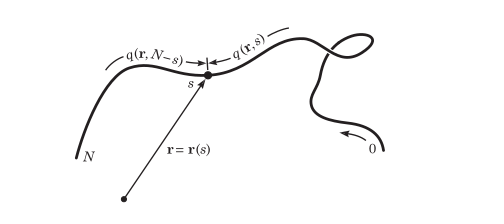
\includegraphics[width=15cm]{Contents/chapter3/figures/32.png}
\caption{说明位于连续高斯链位置s处的段的平均密度的组成公式(\ref{3.59})。轮廓长度s的链段的统计权重$q(\br,s;[w])$在点$r=r(s)$处与具有轮廓长度$N−s$的基本链段的统计权重$q(\br,N−s;[w])$连接。}
\label{figure1}
\end{figure}

\begin{equation}\label{3.60}
\rho(\br;[w])=\int_{0}^{N}\rho(\br,s;[w])~ds
\end{equation}
该公式与微观密度$\hat{\rho}(\br)$和$\hat{\rho}(\br,s)$之间的关系有明显的一致性。

公式(\ref{3.59})的一个特例是特别令人感兴趣的。通过设置$s=0$或$s=N$,可以得到链端段的平均密度。在目前的均聚物的情况下,两个链端是不可区分的,所以总链端密度可以由
\begin{equation}\label{3.61}
\begin{aligned}
\rho_e(\br;[w])&\equiv \rho(\br,0;[w])+\rho(\br,N;[w])\\  &=\frac{2}{VQ[w]}~q(\br,N;[w])
\end{aligned}
\end{equation}
在这个表达式的第二行中,我们使用了$q(\br,0;[w])=1$。因此,在应用规范化$\frac{2}{VQ[w]}$后,传播子$q(\br,N;[w])$可以解释为链端在r位置的平均密度。

公式(\ref{3.56})-(\ref{3.61})中的结果可以很容易地推广到离散高斯链模型。为了简洁起见,我们省略简结的概括,转而转向类似蠕虫的链。在类虫链模型,引入了一个场$w(\br,\bu)$,它与片段位置和取向的微观密度$\hat{\rho}(\br,\bu)$的共轭。因此,对于段位置和取向密度的单链平均值的算子可以被定义为:
\begin{equation}\label{3.62}
\rho(\br,\bu;[w])\equiv <\hat{\rho}(\br,\bu)>_{[w]}=-\frac{\delta lnQ[w]}{\delta w(\br,\bu)}
\end{equation}
这个表达式可以通过离散$Q[w]$的路径积分、对$w(r,u)$的微分和恢复连续极限来计算。结果如下:
\begin{equation}\label{3.63}
\rho(\br,\bu;[w])=\frac{1}{4\pi VQ[w]}\int_{0}^{L_c} q(\br,-\bu,L_c-s;[w])~q(\br,\bu,s;[w])~ds
\end{equation}
这个表达式类似于因式分解性质(\ref{3.41}),因为传播子$q(\br,-u,L_c-s,[w])$描述了“互补”链段的统计权重,其符号为u相反数。

从公式(\ref{3.63})中可以得到几个相关的平均密度。在r或u的两边积分后,得到段方向或位置的平均密度。因此,
\begin{equation}\label{3.64}
\begin{aligned}
\rho(\bu;[w])&\equiv\int \rho(\br,\bu;[w])~d\br \\&=\frac{1}{4\pi VQ[w]}\int  \int_{0}^{L_c}q(\br,-\bu,L_c-s;[w])~q(\br,\bu,s;[w])~d\br ds
\end{aligned}
\end{equation}
和
\begin{equation}\label{3.65}
\begin{aligned}
\rho(\br;[w])&\equiv\int \rho(\br,\bu;[w])~d\bu \\&=\frac{1}{4\pi VQ[w]}\int  \int_{0}^{L_c}q(\br,-\bu,L_c-s;[w])~q(\br,\bu,s;[w])~d\bu ds
\end{aligned}
\end{equation}
提供关于分段位置和位置分布的单独信息。我们还可以避免公式(\ref{3.63})中的链轮廓积分,从而导出在指定等高线位置s处分段位置和方向的平均密度公式为:
\begin{equation}\label{3.66}
\rho(\br,\bu,s;[w])=\frac{1}{4\pi VQ[w]}~q(\br,-\bu,L_c-s;[w])~q(\br,\bu,s;[w])
\end{equation}
最后,该表达式可用于推导出链端段位置和方向的平均密度。
\begin{equation}\label{3.67}
\begin{aligned}
\rho_e(\br,\bu;[w])&\equiv \rho(\br,\bu,0;[w])+\rho(\br,\bu,L_c;[w])\\ &=\frac{1}{4\pi VQ[w]}[q(\br,-\bu,L_c;[w])+q(\br,\bu,L_c;[w])]
\end{aligned}
\end{equation}


对于棒状聚合物模型,段位置和取向的密度算子与蠕虫链的密度算子一致。见公式(\ref{3.62})。采用公式(\ref{3.45})的一阶泛函导数将导致:
\begin{equation}\label{3.68}
\rho(\br,\bu;[w])=\frac{1}{4\pi VQ[w]}\int_{0}^{L_c}\exp[-\int_{0}^{L_c}w (\br+(s^{'}-s)\bu,\bu)~ds^{'}]~ds
\end{equation}
通过定义棒状聚合物的传播子$q(r,u,s;[w])$
\begin{equation}\label{3.69}
q(\br,\bu,s;[w])\equiv \exp[-\int_{0}^{s}w(\br-s^{'}\bu,\bu)~ds^{'}]
\end{equation}
假设$w(\br,\bu)=w(\br,-\bu)$,则公式(\ref{3.68})中给出的棒状聚合物密度算子可以与公式(\ref{3.63})蠕虫链的表示形式完全相似。

单链密度算子范畴下的最后一个话题是段密度的高阶矩。对象$Q[w]$和$ln Q[w]$可视为生成泛函(Van Kampen1981),因为这些量的泛函导数分别产生了微观单链密度的矩和累积量(见附录B)。实际上,对于高斯链模型的一阶矩可以表示为:
\begin{equation}\label{3.70}
<\hat{\rho}(\br)>_{[w]}=-\frac{\delta lnQ[w]}{\delta w(\br)}=-\frac{1}{Q[w]}\frac{\delta Q[w]}{\delta w(\br)}
\end{equation}
同样地,从规范化的配分函数和单链平均的定义中看出,微观密度的第二矩是由Q的第二泛函导数给出的。
\begin{equation}\label{3.71}
<\hat{\rho}(\br)\hat{\rho}(\br^{'})>_{[w]}=\frac{1}{Q[w]}\frac{\delta^2 Q[w]}{\delta w(\br)\delta  w(\br^{'})}
\end{equation}
第二累积矩同样由lnQ的第二泛函导数来表示:
\begin{equation}\label{3.72}
<\hat{\rho}(\br)\hat{\rho}(\br^{'})>_{[w]}-<\hat{\rho}(\br)>_{[w]}<\hat{\rho}(\br^{'})>_{[w]}=\frac{\delta^2 lnQ[w]}{\delta w(\br)\delta w(\br^{'})}
\end{equation}
我们回顾了公式(\ref{3.53})和(\ref{3.55})给出了链传播子q与微观段密度的第一矩之间高斯链模型的明确关系。传播子和矩之间的这种联系可以扩展到高阶矩,方法是采用附加的函数导数,从而在附加点上考虑链的统计权重。例如,在连续高斯链的情况下,二阶矩,或密度-密度相关函数,给出:
\begin{equation}\label{3.73}
\begin{aligned}
<\hat{\rho}(\br)\hat{\rho}(\br^{'})>_{[w]}&=\frac{1}{VQ[w]}\int_{0}^{N} \int_{0}^{s}q(\br,N-s;[w])\\&\times g(\br,\br^{'},s-s^{'};[w])~q(\br^{'},s^{'};[w])~dsds^{'}\\&+\frac{1}{VQ[w]}\int_{0}^{N} \int_{0}^{s^{'}}q(\br^{'},N-s^{'};[w])\\&\times g(\br^{'},\br,s^{'}-s;[w])~q(\br,s;[w])~ds^{'}ds
\end{aligned}
\end{equation}
这个方程中出现的函数$g(\br,s,[w])$是一个新的链传播子,它满足公式(\ref{3.25}),但服从$\delta$函数初始条件,即:
\begin{equation}\label{3.74}
\frac{\partial}{\partial s}~g(\br,\br^{'},s;[w])=\frac{b^2}{6}\bigtriangledown^2~g(\br,\br^{'},s;[w])-w(\br)~g(\br,\br^{'},s;[w])
\end{equation}
\begin{equation}\label{3.75}
g(\br,\br^{'},0;[w])=\delta(\br-\br{'})
\end{equation}
因此,$g(\br,\br^{'},s;w)$是公式(\ref{3.25})的格林函数(或基本)解,如图\ref{figure2}所示,这个传播子生成聚合物的长度s内部截面的统计权重,它起源于r位,终止于r位置。
\begin{figure}[h]
\centering
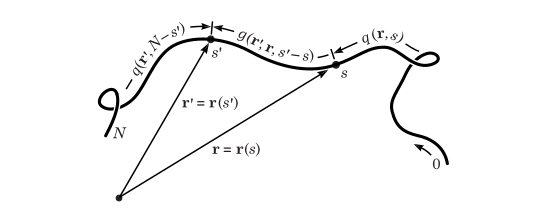
\includegraphics[width=15cm]{Contents/chapter3/figures/33.png}
\caption{解释了连续高斯链段密度-密度相关函数的合成公式(\ref{3.73})(仅最后一项)。轮廓长度-s的链端截面的统计权重$q(\br,s)$在点$\br=\br(s)$处连接到传播子$g(\br^{'},\br,s^{'}-s)$。传播子描述与长度为$s^{'}-s$的内部链段相关的统计权重,从$\br=\br(s^{'})$开始,结束于$r=r(s)$。最后“互补”链端截面的统计权重为$q(\br,N-s^{'})$。}
\label{figure2}
\end{figure}

图\ref{figure2}描述了公式(\ref{3.72})的物理解释。该方程可用于计算具有势$w(\br)$的连续高斯链段密度的二阶矩。虽然这类高阶密度相关函数的公式便于近似解析计算,但在高精度精度中应该避免。这是因为计算两点传播子(如$g(\br,s,[w])$所付出的代价)。如果使用M个网格点或谱分量来求解空间自由度,请参见第3.6节,g的数值计算至少需要$M^2$算子。在三维模拟中, 使用这样的$O(M^2)$缩放的计算令人望而却步, 其中M大到$10^6-10^7$.
\subsection{应力算子}
另一个重要的量是放置在不均匀环境中的聚合物链所产生的平均弹性应力。弹性应力算子(Stress operators)可以定义为:
\begin{equation}\label{3.76}
\sigma(\mathbf{\br};[w,\epsilon])\equiv<\hat{\sigma}(\br)>_{[w,\epsilon]}
\end{equation}
其中,单链平均是根据公式(\ref{3.47})计算的。用离散高斯链模型计算这个表达式的右边会产生两个不同的表达式,
\begin{equation}\label{3.77}
\begin{aligned}
\sigma(\br;[w,\epsilon])&=\frac{\int {\hat{\sigma}}(\br)~\exp[-\beta U(\br^{N+1})-\beta U_{el}(\br^{N+1})]~d\br^{N+1}}{\int \exp[-\beta U(\br^{N+1})-\beta U_{el}(\br^{N+1})]~d\br^{N+1}}\\&=\frac{\int \hat{\sigma}(\br)~\exp[-\beta U(\br^{N+1})-\beta U_{el}(\br^{N+1})]~d\br^{N+1}}{Q[w,\epsilon]~\int \exp[-\beta U_0(\br^{N+1})-\beta U_{el}(\br^{N+1})]~d\br^{N+1}}
\end{aligned}
\end{equation}
第二个是最方便计算的。在最后一个表达式中插入微观应力运算符公式(\ref{3.11})的显式形式将导致:
\begin{equation}
\begin{aligned}\label{3.78}
\sigma_{\alpha \gamma}(\br;[w,\epsilon])&=\frac{3k_BT}{b^2VQ[w,\epsilon]} \int (\br^{'}-\br)_{\alpha} (\br^{'}-\br)_{\gamma} \varPsi (\br^{'}-\br;[\epsilon])\\&\times \sum_{j=0}^{N-1}q(\br^{'},N-j-1;[w,\epsilon])~q(\br,j;[w,\epsilon])~d\br^{'}
\end{aligned}
\end{equation}
其中函数$\varPsi (\br^{'}-\br;[\epsilon])$是在公式(\ref{3.14})中定义的。这个表达式可以通过先解公式(\ref{3.15})-(\ref{3.17})得到传播子$q(\br,j;[w,\epsilon])$和配分函数$Q[w,\epsilon]$然后指定公式(\ref{3.78})中的被积和求和,其余运算可以数值计算出来。

在连续高斯链模型的基础上,导出了应力算子的类似表达式(Fredrickson,2002)。对于非均匀应变场,这个表达式是相当复杂的,因此不在这里再现。在均匀应变$\epsilon$的情况下,得到$^{19}$.
\begin{equation}\label{3.79}
\sigma(\br;[w,\epsilon])=\frac{k_BTb^2}{3VQ[w,\epsilon]}\int_{0}^{N} q(\br,s;[w,\epsilon])~\nabla \nabla q(\br,N-s;[w,\epsilon])~ds
\end{equation}
应力算子的这个表达式表明,在空间变化的化学势$w(\br)$存在下,弹性应力是各向异性的和非均匀的。应力各向异性是由沿链等高线积分的并矢量$q\nabla \nabla q$来表示的。泰勒和莫尔斯在研究嵌段共聚物中间相的线弹性性质时,推导出了密切相关的公式(Tyler and morse,2003a;Tyler and Morse,2003b)。方程(\ref{3.79})对于研究细观结构聚合物流体中链拉伸的不均匀分布特别有用。

\section{其他的结构}
{\color{red}\begin{center}
        龚欣
    \end{center}}

前一节讲了最简单的聚合物结构-线性均聚物。对于各种各样的体系结构包括那些具有实际和学术意义的体系都可以得到类似的结果。在本节中,我们导出了在空间变化势作用下分支均聚物(branched homopolymers)、嵌段共聚物和接枝共聚物(block and graft copolymers)的显式表达式。像聚合物的结构是化学无序的,如随机分支均聚物(randomly branched homoploymers)、统计共聚物(statistical copolymers)和随机接枝共聚物(randomly grafted copolymers)的讨论,将推迟到$4.7$节讨论。
\subsection{分支均聚物}
作为分支均聚物的第一个例子,我们考虑一个$3$臂星形均聚物,如图\ref{三臂星形均聚物}所示。每个臂采用连续高斯链模型描述并且有任意的长度。相应的,每条链的聚合度分别是$N_1$,$N_2$,$N_3$。假设每个臂上的片段经历一个化学势场$w (\br)$。在这种情况下,因为每个臂在化学上是相同的,所以只需要一种化学势。
\begin{figure}[H]
\centering
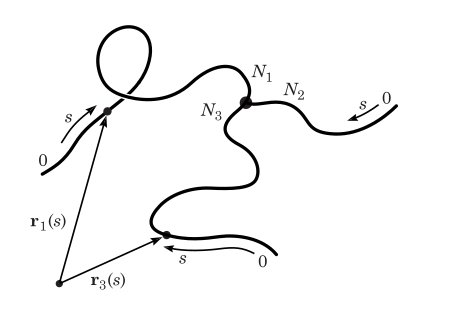
\includegraphics[scale=0.7]{Contents/chapter3/figures/34.png}
\caption{连续高斯链模型中的$3$臂星形聚合物。聚合度分别为$N_1$,$N_2$,$N_3$的三个支臂连接在一个中心支点上。第$j$个臂的构型用空间曲线$\br_j(s)$描述,$s\in [0,N_j]$。}
\label{三臂星形均聚物}
\end{figure}

如图\ref{三臂星形均聚物}所示,第$j$个臂$(j=1,2,3)$的构型由空间曲线$\br_j(s)$描述,其中路径参数$0\leq s\leq N_j$,这是从每个臂的自由端测量。在支点处,臂满足$\br_1(N_1)=\br_2(N_2)=\br_3(N_3)$。

第$3.1.2$节关于线性均聚物的公式可以很容易地推广到目前的情况。微观段密度(microscopic segment density)可以写成
\begin{equation}
\tilde{\rho}(\br)=\sum_{j=1}^3 \int_{0}^{N_j}\,\rho(\br-\br_{j}(s)) \mathrm{d}s
\end{equation}
与施加的化学势$w (\br)$的相关的势能是整个聚合物形状$\br$的一个泛函,$\br(s)\equiv \left\{ \br_1(s),\br_2(s),\br_3(s) \right\}:$
\begin{equation}
\beta U_1[\br,w]=\int w(\br^{'})\tilde{\rho}(\br^{'})\mathrm{d}\br^{'}
\end{equation}
归一化的配分函数$Q[w]$也可以表示为路径积分的比率
\begin{equation}
Q[w]\equiv \frac{Z[w]}{Z_0}=\frac{\int^{*}~\exp (-\beta U_0[\br]-\beta U_1[\br,w])\calD\br}{\int^{*} \exp (-\beta U_0[\br]) \calD\br} \label{82}
\end{equation}
其中理想链的势能
\begin{equation}
\beta U_0[\br]=\frac{3}{2b^2}\sum_{j=1}^3\int_{0}^{N_j} \left| \frac{d\br_j(s)}{ds} \right|^2 \mathrm{d}s
\end{equation}
和$\int^{*}\calD\br$是受支点约束的三个臂上的路径积分
\begin{equation}
\int^{*}\calD\br\equiv \int \delta (\br_1(N_1)-\br_2(N_2))\delta (\br_2(N_2)-\br_3(N_3)) \calD\br  \label{83}
\end{equation}
方程(\ref{82})中的路径积分可以通过离散这三条路径来计算,这三条路径对应于星臂的构型,从而得到了一个类似于线性均聚物方程(\ref{3.21})的表达式。方程(\ref{83})的约束是通过建立从三个臂的自由端开始,在公共分支点的位置终止的路径积分,因此,由乘积$q(\br,N_1)q(\br,N_2)q(\br,N_3)$给出了有支点的星形聚合物关于$\br$的统计重量,其中传播子(propagators)满足方程(\ref{3.25})-(\ref{3.26})。配分函数是
\begin{equation}
Q[w]=\frac{1}{V}\int ~q(\br,N_1;[w])q(\br,N_2;[w])q(\br,N_3;[w]) \mathrm{d}\br
\end{equation}
应该注意,应用这个公式并不需要求解扩散方程(\ref{3.25})的三个独立解,而是一个,因为对$0\leq s\leq N_{\max}$(其中$N_{\max}$是$N_j$中最大的)的$q(\br,s;[w])$足以评估全部的三个传播子。

$3$臂星形均聚物的段密度算子可与线性聚合物的方程(\ref{3.55})类比得出。在连续高斯链模型中,我们有
\begin{equation}
\rho(\br;[w])=-\frac{1}{Q[w]}\frac{\delta Q[w]}{\delta w(\br)}=\rho _1(\br;[w])+\rho _2(\br;[w])+\rho _3(\br;[w])
\end{equation}
这里的$\rho _j(\br;[w])$表示星的第$j$个臂对平均段密度的贡献。其中
\begin{equation}
\rho _{j}(\br;[w])=\frac{1}{VQ[w]} \int_{0}^{N_j}\,q_{j}(\br,N_{j}-s;[w])q(\br,s;[w]) \mathrm{d}s \label{87}
\end{equation}
“互补传播子”$q_{j}(\br,s;[w])$满足与$q$相同的扩散方程,但具有不同的初始条件,即
\begin{equation}
\frac{\partial}{\partial s}q_j(\br,s;[w])=\frac{b^2}{6}q_j(\br,s;[w])-w(\br)q_j(\br,s;[w]) \label{88}
\end{equation}
\begin{equation}
q_j(\br,0;[w])=
\begin{cases}
q(\br,N_2;[w])q(\br,N_3;[w]), & j=1 \\
q(\br,N_1;[w])q(\br,N_3;[w]), & j=2 \\
q(\br,N_1;[w])q(\br,N_2;[w]), & j=3  \label{89}
\end{cases}
\end{equation}

\begin{figure}[H]
\centering
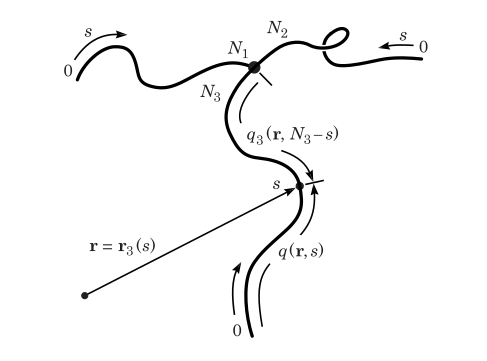
\includegraphics[scale=0.7]{Contents/chapter3/figures/35.png}
\caption{$3$臂星形均聚物的密度算子$\rho _3(\br;[w])$的构造。这个密度由统计权重$q(\br,s;[w])$组成,代表臂$3$的自由端,具有互补的传播子$q_3(\br,N_3-s;[w])$,表示臂与分支点连接的部分的统计重量。在满足初始条件(\ref{89}),后者是通过对远离分支点的方程(\ref{88})进行积分获得的。}
\label{三臂星形图像}
\end{figure}

图(\ref{三臂星形图像})说明了当$j=3$时的臂的平均密度$\rho _3$的方程(\ref{87})的物理解释。臂必须通过点$\br=\br_3(s)$,其中$s$是从臂的自由端测量的路径参数。与这种臂构型相关联的是统计重量$q(\br,s;[w])$的乘积,它表示臂的悬空(自由)末端,以及权重$q_{3}(\br,N_{3}-s;[w])$,表示与星其余部分相连的臂段。互补传播子$q_3$是从分支点开始,在$N_3-s$的总的路径距离上对方程(\ref{88})积分得出的。这种积分的初始条件是在分支点与剩余的两个臂相关联的统计权重,它可以用两个$q$传播子的乘积表示,如方程(\ref{89})所述。

上述结果可以很容易地推广到具有任意臂数的星形均聚物。最一般情况是具有不同长度且$p\geq3$臂的星形均聚物,总段密度算子的求值要求扩散方程的$p+1$个解:一种是从长度为$N_{\max}$(最长臂长)的链获得$q$,另一解为$p$互补传播子$q_j(\br,s;[w])$,$s\in [0,N_j]$。在具有等臂长的$p$星聚合物的特殊情况下,由于所有互补传播子相同,计算量大大减少。因此,在这种高对称性的特殊情况下,只需要扩散方程的两个解。

\begin{figure}[H]
\centering
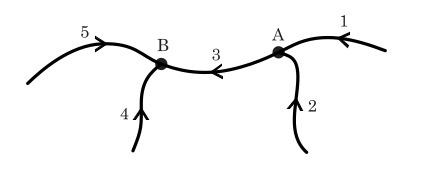
\includegraphics[scale=0.7]{Contents/chapter3/figures/36.png}
\caption{另一个例子,一个分支均聚物由$5$部分组成,$1-5$连接在两个分支点$A$和$B$上。箭头表示一个(任意)的积分方向,以建立聚合物的统计重量。}
\label{AB嵌段}
\end{figure}

作为分支均聚物的第二个例子,我们考虑了图(\ref{AB嵌段})所示的支化聚合物。聚合物由标记为$1-5$的五个节段组成,分别连接在$A$和$B$的两个支点处。第$j$节的聚合度用$N_j$表示。没有什么特殊的方法来建立这样一种聚合物的统计重量,但各种替代品提供了同等的结果。为了说明如何通过在分支点$B$处合成传播子来计算归一化配分函数$Q[w]$,图(\ref{AB嵌段})中聚合物截面上的箭头指示了用于计算传播子的积分方向,箭头是任意分配的。有图明显看出,在$B$处,三个方向都聚焦在此,通过将第$3$,$4$和$5$段中的传播子组合在一起可以得到$Q[w]$
\begin{equation}
Q[w]=\frac{1}{V}\int q_3(\br,N_3;[w])q(\br,N_4;[w])q(\br,N_5;[w]) \mathrm{d}\br
\end{equation}
第$4$段和第$5$段中,$q$传播子在自由链端开始,因此满足方程(\ref{3.25})-(\ref{3.26})。相反,第3节的$q_3$传播子在分支点$A$处开始,从而满足初始条件下的扩散方程(\ref{88})
\begin{equation}
q_3(\br,0;[w])=q(\br,N_1;[w])q(\br,N_2;[w])
\end{equation}
这个初始条件提供了与支点$A$处的链节$1$和$2$相关联的统计权重。

类似的表达式可以写成对这种支化聚合物的平均段密度的各种贡献。例如,第$3$段对段密度运算符的贡献可以表示为
\begin{equation}
\rho(\br;[w])=\frac{1}{VQ[w]}\int _{0}^{N_3} q_{3c}(\br,N_3-s;[w])q_3(\br,s;[w]) \mathrm{d}s
\end{equation}
其中$q_3(\br,s;[w])$是从分支点$A$出发的传播子。“互补”传播子$q_{3c}(\br,N_3-s;[w])$在分支点$B$处发起,并扩展路径距离$N_3-s$在$\br$点加入传播子$q_{3c}$。在初始条件下,$q_{3c}$满足方程(\label{传播子求导})
\begin{equation}
q_{3c}(\br,0;[w])=q(\br,N_4;[w])q(\br,N_5;[w])
\end{equation}
它提供了分支点$B$处的分支$4$和$5$的统计权重。

利用相关的参数,可以构造具有外势的任意结构的分支均聚物的配分函数以及密度算子和应力算子。这种表达式也可以推广到连续高斯链之外,在离散和蠕虫状链模型的背景下处理分支聚合物。

\subsection{嵌段接枝共聚物}
嵌段共聚物和接枝共聚物是聚合物工业中特别重要的材料,与纳米技术特别相关。由于这种聚合物是由两个或两种以上的在化学性质上不同的部分(“blocks”或“grafts”)组成的,它们在势场存在的情况下的统计力学比均聚物更丰富。

我们首先讨论$AB$两嵌段共聚物的连续高斯链模型,如图(\ref{图37})所示。共聚物的总聚合物度指数为$N$,$0\leq s \leq fN$(实线)段由$A$型段组成,$fN \leq s \leq N$(虚线)由$B$型段组成。$f$是表示$A$链长度与总链长度之比的参数,如果进一步定义$A$和$B$段具有相等的体积,则$f$对应于链上$A$型段的平均体积分数。与共聚物的$A$和$B$段相对应的统计段长度分别是$b_A$和$b_B$。我们还引入了外部化学势场$w_A(\br)$和$w_B(\br)$,它们分别作用于共聚物的$A$和$B$段。

\begin{figure}[H]
\centering
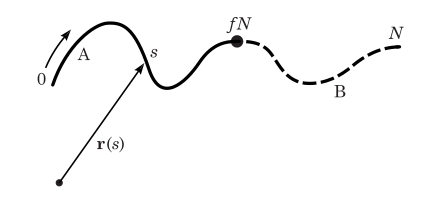
\includegraphics[scale=0.7]{Contents/chapter3/figures/37.png}
\caption{$AB$两嵌段共聚物的连续高斯链模型。$0\leq s \leq fN$(实线)段由$A$型段组成,$fN \leq s \leq N$(虚线)由$B$型段组成。$f$是表示$A$链长度与总链长度之比的参数。}
\label{图37}
\end{figure}

这种两嵌段共聚物的拉伸势能可以表示为
\begin{equation}
\beta U_0[\br]=\int_{0}^{N} \frac{3}{2[b(s)]^2}\left| \frac{d\br(s)}{ds} \right|^2 \mathrm{d}s
\end{equation}
这里
\begin{equation}
b(s)\equiv
\begin{cases}
b_A, & 0\leq s \leq fN \\
b_B, & fN \leq s \leq N\\
\end{cases}
\end{equation}
同样,与外部势$w_A$和$w_B$相关的势能可以写为
\begin{equation}
\beta U_1[\br,w_A,w_B]=\int [w_A(\br^{'})\tilde{\rho}_{A}(\br^{'})+w_B(\br^{'})\tilde{\rho}_{B}(\br^{'})] \mathrm{d}\br^{'}
\end{equation}
其中$\tilde{\rho} _A$和$\tilde{\rho} _B$是由下面公式定义的微观段密度
\begin{equation}
\tilde{\rho} _A(\br)=\int _0^{fN} ~\delta(\br-\br(s)) \mathrm{d}s,~~~\tilde{\rho} _B(\br)=\int _{fN}^{N} ~\delta(\br-\br(s)) \mathrm{d}s
\end{equation}
此两嵌段的归一化配分函数表达式是
\begin{equation}
Q[w_A,w_B]\equiv\frac{Z[w_A,w_B]}{Z_0}=\frac{\int ~\exp(-\beta U_0[\br]-\beta U_1[\br,w_A,w_B]) \calD\br}{\int ~\exp(-\beta U_0[\br]) \calD\br}
\end{equation}
前几节所描述的方法也可于将分配函数、密度和应力算子与满足Fokker-Planck方程的链传播算子联系起来。在这种情况下,由共聚物的$s=0$($A$节点)端引发的传播子$q(\br,s;[w_A,w_B])$满足扩散方程
\begin{equation}
\frac{\partial}{\partial s}q(\br,s;[w_A,w_B])=\frac{[b(s)]^2}{6}\triangledown ^2q(\br,s;[w_A,w_B])-w(\br,s)q(\br,s;[w_A,w_B]) \label{3.99}
\end{equation}
这里
\begin{equation}
w(\br,s)\equiv
\begin{cases}
w_A(\br), & 0\leq s \leq fN \\
w_B(\br), & fN \leq s \leq N\\
\end{cases}
\end{equation}
方程(\ref{3.99})在初始条件$q(\br,0;[w_A,w_B])=1$的情况下求解。

另一个有用的量是从共聚物的$s=N$末端出发的互补传播子$q_c(\br,s;[w_A,w_B])$。通过建立从$B$端开始的共聚物统计重量,可以得$q_c$满足类似的扩散方程
\begin{equation}
\frac{\partial}{\partial s}q_c(\br,s;[w_A,w_B])=\frac{[b_c(s)]^2}{6}\triangledown ^2q_c(\br,s;[w_A,w_B])-w_c(\br,s)q_c(\br,s;[w_A,w_B]) \label{101}
\end{equation}
这里
\begin{equation}
b_c (s)\equiv
\begin{cases}
b_B, & 0\leq s \leq (1-f)N \\
b_A, & (1-f)N \leq s \leq N\\
\end{cases}
\end{equation}
和
\begin{equation}
w_c (\br,s)\equiv
\begin{cases}
w_B(\br), & 0\leq s \leq (1-f)N \\
w_A(\br), & (1-f)N \leq s \leq N\\
\end{cases}
\end{equation}
用$q_c(\br,0;[w_A,w_B])=1$,方程(\ref{101})在$s$中也是向前积分的。		

使用上面的传播子,可以用两种等效的方法计算配分函数:
\begin{equation}
\begin{aligned}
Q[w_A,w_B] & = \frac{1}{V}\int q(\br,N;[w_A,w_B]) \mathrm{d}\br \\
&=\frac{1}{V}\int q_c(\br,N;[w_A,w_B]) \mathrm{d}\br \\
\end{aligned}	
\end{equation}
换句话说,两嵌段共聚物的传播子可以从分子的$A$端或$B$端建立,从而得到整个链的等效统计重量。因此,只需求解方程(\ref{3.99})或方程(\ref{101})就能计算配分函数$Q[w_A,w_B]$。

相反,计算两嵌段共聚物的密度算子需要两个链传播子的信息。$A$段和$B$段的平均密度是由现在熟悉的前向和后向传播子组成的过程构造的,从而得到表达式
\begin{equation}
\begin{aligned}
\rho _A(\br;[w_A,w_B]) & =-\frac{1}{Q[w_A,w_B]}	\frac{\delta Q[w_A,w_B]}{\delta w_A(\br)} \\
& =\frac{1}{VQ[w_A,w_B]} \int _{0}^{fN}\,q_c(\br,N-s;[w_A,w_B])q(\br,s;[w_A,w_B]) \mathrm{d}s~ \\
\end{aligned}	
\end{equation}

\begin{equation}
\begin{aligned}
\rho _B(\br;[w_A,w_B]) & =-\frac{1}{Q[w_A,w_B]}	\frac{\delta Q[w_A,w_B]}{\delta w_B(\br)} \\
& =\frac{1}{VQ[w_A,w_B]} \int _{fN}^{N}\,q_c(\br,N-s;[w_A,w_B])q(\br,s;[w_A,w_B])\mathrm{d}s~ \\
\end{aligned}	
\end{equation}
上述结果在嵌段共聚物理论中都是众所周知的(Helfand and Wasserman,1976;Hong and Noolandi,1981;Matsen和Schick,1994a)。

作为最后一个例子,我们讨论$A_2B$接枝共聚物的情况,其结构如图(\ref{3.8})所示。这样的分子可以被看作是有一个$A$主链与一个单一的$B$块“嫁接”到它。或者,该共聚物可以被看作是一种星共聚物有两个$A$臂,分别是$A_1$和$A_2$,和一个$B$臂。从后一种观点出发,分别用$N_{A1}$,$N_{A2}$和$N_B$来表示臂的聚合程度。为了简单起见,采用了连续高斯链模型。

\begin{figure}[H]
\centering
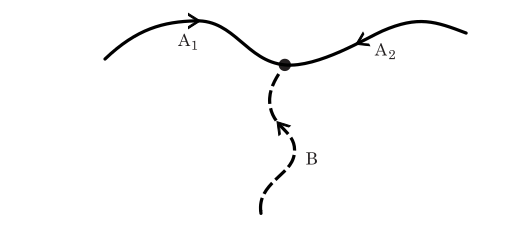
\includegraphics[scale=0.7]{Contents/chapter3/figures/38.png}
\caption{一个$A_2B$接枝共聚物的连续高斯链模型。该共聚物可视为$B$均聚物链接枝到均聚物主链(实线)$A$上,也可视为具有两个$A$臂和$1$个$B$臂的星形共聚物。箭头表示建立该分子的统计重量一个特定(任意)方向。}
\label{3.8}
\end{figure}		

我们需要两个不同的链传播子来构造图(\ref{3.8})所示的接枝共聚物的配分函数$Q[w_A,w_B]$。它们对应于从共聚物臂的自由端开始生长一段$A$或$B$型均聚物链。传播子$q_A(\br,s;[w_A])$和$q_B(\br,s;[w_A])$满足
\begin{equation}
\frac{\partial}{\partial s}q_K(\br,s;[w_K])=\frac{b_K^2}{6}\triangledown ^2q_K(\br,s;[w_K])-w_K(\br)q_K(\br,s;[w_K]) \label{107}
\end{equation}
上式$K=A$或$B$.方程(\ref{107})的求解条件是$q_K(\br,0;[w_K])=1$。有了这些定义,接枝共聚物的总统计重量是通过在分支点上连接三个这样的传播子来构造的,这意味着配分函数可以写成
\begin{equation}
Q[w_A,w_B]=\frac{1}{V}\int ~q_A(\br,N_{A1};[w_A])q_A(\br,N_{A2};[w_A])q_B(\br,N_B;[w_B]) \mathrm{d}\br
\end{equation}

密度算子可以用类似于分支均聚物和两嵌段共聚物的方法来构造.例如,通过将(正前)$B$传播子$q_B$与从支点发起的互补(向后)$B$传播子$q_{B_c}(\br,s;[w_A,w_B])$组合,可获得接枝共聚物的平均段$B$密度。后一个传播子满足
\begin{equation}
\frac{\partial}{\partial s}q_{B_c}(\br,s;[w_A,w_B])=\frac{b_B^2}{6}\triangledown ^2q_{B_c}(\br,s;[w_A,w_B])-w_B(\br,s)q_{B_c}(\br,s;[w_A,w_B])
\end{equation}
满足
\begin{equation}
q_{B_c}(\br,0;[w_A,w_B])=q_A(\br,N_{A1};[w_A])q_A(\br,N_{A2};[w_A])
\end{equation}
这个初始条件提供了在支点的两个$A$臂的统计重量。在此基础上,$A_2B$接枝共聚物$B$段的平均密度是
\begin{equation}
\begin{aligned}
\rho _B(\br;[w_A,w_B]) & =-\frac{1}{Q[w_A,w_B]}	\frac{\delta Q[w_A,w_B]}{\delta w_B(\br)} \\
&= \frac{1}{VQ[w_A,w_B]} \int _{0}^{N_B}\,~q_{B_c}(\br,N_B-s;[w_A,w_B])q_B(\br,s;[w_B])\mathrm{d}s \\
\end{aligned}	
\end{equation}
对于两个$A$形臂中任何一个$A$形臂所贡献的类型段的平均密度,也可以编写类似的表达式。

\subsection{近似方案}
在本章前三节中,重点关注的是推导外势作用下单链模型配分函数的精确表达式以及平均性质.大多数情况下,这些表达式并不适合进行精确分析.虽然完整的数值解非常重要,但若能得到一些近似解析表达式
(比如配分函数$Q[w]$和密度算子$\rho(\br ;[w])$的近似解析式)也非常有帮助.这些可用于聚合物流体的多链场理论的分析研究.更重要的,理解单链平均值和算子的渐近行为可以帮助发展多链场理论的有效数值方法.

本节将集中讨论推导配分函数和单链平均值的系统扰动展开的方法.这种渐近方法最直接地应用于Fokker-Planck方程可用的连续链模型.因此,对于连续高斯链和类虫链,可以利用偏微分方程正则摄动和奇异摄动方法的大量文献.在本节中,我们将注意力限制在连续链模型上,并尝试提供一个微扰展开的指南.
\subsection{弱非均匀性展开}
当应用的势场$w$具有振幅较弱的不均匀性时,可以得到一个有用的微扰展开式.

为了定义此情形,引入势的体积平均值:
\begin{equation}
w_0\equiv \frac{1}{V} \int w(\br )\,\mathrm{d}\br 
\end{equation}
并重新定义$w(\br )$:
\begin{equation}
w(\br )=w_0+\omega(\br ) \label{3.113}
\end{equation}
其中,$\omega(\br )$用于定义场的非均匀部分.
当非均匀性很弱时,描述振幅特征的小参数$\epsilon_a$ $(|\epsilon_a| \ll 1)$可以从$\omega(\br )$中提取出来,即方程(\ref{3.113})改写为:
$$w(\br )=w_0+\epsilon_a \omega(\br )$$

对于聚合物的连续高斯链模型,Fokker-Planck方程及其初始条件为:
\begin{equation}
\frac{\partial}{\partial s} q(\br ,s) = \frac{b^2}{6} \bigtriangledown^2 q(\br ,s) -w_0 q(\br ,s) -\epsilon_a \omega(\br ) q(\br ,s) \label{3.114}
\end{equation}
\begin{equation}
q(\br ,0) = 1 \label{3.115}
\end{equation}
其中并不标记$q$关于$w = w_0+\epsilon_a \omega$的函数依赖性.方程(\ref{3.114})的右边中与$w_0$成比例的项可以用以下代换消掉:
\begin{equation}
q(\br ,s) = e^{-w_0 s} p(\br ,s) \label{3.116}
\end{equation}
从而得到:
\begin{equation}
\frac{\partial}{\partial s} p(\br ,s) = \frac{b^2}{6} \bigtriangledown^2 p(\br ,s) -\epsilon_a \omega(\br ) p(\br ,s) \label{3.117}
\end{equation}
\begin{equation}
p(\br ,0) = 1 \label{3.118}
\end{equation}

假设$p(\br ,s)$可以写为以下形式并由此考虑弱非均匀性展开:
\begin{equation}
p(\br ,s) \sim \sum_{j=o}^{\infty} {\epsilon_a}^j p^{(j)} (\br ,s) \label{3.119}
\end{equation}
其中$p^{(j)} (\br ,s)$与$\epsilon_a$无关.方程(\ref{3.119})中我们用$\sim$表示渐近展开.因此,方程(\ref{3.119})中右边的无穷级数既可以收敛也可以发散.即便不收敛,其在截断形式下仍可以在$\epsilon_a$足够小时近似于$p(\br ,s)$.

通过把方程(\ref{3.119})代入方程(\ref{3.117})-(\ref{3.118})计算$p^{(j)}$,并按照$\epsilon_a$的阶数对应计算项.
$$\frac{\partial}{\partial s} (\sum_{j=o}^{\infty} {\epsilon_a}^j p^{(j)} (\br ,s)) = \frac{b^2}{6} \bigtriangledown^2 (\sum_{j=o}^{\infty} {\epsilon_a}^j p^{(j)} (\br ,s)) - \omega(\br ) (\sum_{j=o}^{\infty} {\epsilon_a}^{j+1} p^{(j)} (\br ,s))$$

对于首阶$O({\epsilon_a}^0)$,有:
\begin{equation}
\frac{\partial}{\partial s} p^{(0)}(\br ,s) = \frac{b^2}{6} \bigtriangledown^2 p^{(0)}(\br ,s)
\end{equation}
\begin{equation}
p^{(0)}(\br ,0) = 1
\end{equation}
其有平凡解$p^{(0)}(\br ,s) = 1$.

对于$O(\epsilon_a)$,有:
\begin{equation}
\frac{\partial}{\partial s} p^{(1)}(\br ,s) = \frac{b^2}{6} \bigtriangledown^2 p^{(1)}(\br ,s)-\omega(\br ) p^{(0)}(\br ,s)
\end{equation}
\begin{equation}
p^{(1)}(\br ,0) = 0
\end{equation}
如果所考虑的系统不是无界的或受受周期性边界条件约束的,那么这个初值问题容易通过空间傅里叶变换来解决.

假设$\omega(\br )$的傅里叶变换存在,记为$\hat{\omega}(\mathbf{k})$.
由$p^{(0)}(\br ,s) = 1$,可得
$$\frac{\partial}{\partial s} p^{(1)}(\br ,s) = \frac{b^2}{6} \bigtriangledown^2 p^{(1)}(\br ,s)-\omega(\br )$$
两边对$p^{(1)}(\br ,s)$关于$\br $作傅里叶变换,则
$$\frac{\partial}{\partial s}\hat{p}^{(1)}(\mathbf{k},s) = \frac{-k^2 b^2}{6} \hat{p}^{(1)}(\mathbf{k},s)-\hat{\omega}(\mathbf{k})$$
(其中$F(f^{(n)}(x)) = (ik)^n F(f(x))$)
从而$$(\hat{p}^{(1)}(\mathbf{k},s)e^{\frac{k^2 b^2 s}{6}})' = -\hat{\omega}(\mathbf{k}) e^{\frac{k^2 b^2 s}{6}}$$
两边关于s求积分得
$$\hat{p}^{(1)}(\mathbf{k},s)e^{\frac{k^2 b^2 s}{6}}-\hat{p}^{(1)}(\mathbf{k},0) = -\hat{\omega}(\mathbf{k}) \int_{0}^{s} e^{\frac{k^2 b^2 t}{6}}\, \mathrm{d}t$$
又$\hat{p}^{(1)} (\mathbf{k},0) = 0$,所以
$$\hat{p}^{(1)}(\mathbf{k},s) = -\frac{6}{k^2 b^2} (1-e^{-\frac{k^2 b^2 s}{6}}) \hat{\omega}(\mathbf{k})$$
将上式记为:
\begin{equation}
\hat{p}^{(1)}(\mathbf{k},s) = -\hat{h_2}(\mathbf{k},s) \hat{\omega}(\mathbf{k})
\end{equation}
其中
\begin{equation}
\hat{h_2}(\mathbf{k},s) = \frac{6}{k^2 b^2} (1-e^{-\frac{k^2 b^2 s}{6}})
\end{equation}

类似的,对于$O({\epsilon_a}^2)$,有
\begin{equation}
{\hat{p}}^{(2)}(\mathbf{k},s) = \frac{1}{V} \sum_{\mathbf{k}'} \hat{h_3}(\mathbf{k},\mathbf{k}',s)\hat{\omega}(\mathbf{k}-\mathbf{k}')\hat{\omega}(\mathbf{k}')
\end{equation}
其中
\begin{equation}
\hat{h_3}(\mathbf{k},\mathbf{k}',s) = \frac{36}{b^4 k^2 {|\mathbf{k}-\mathbf{k}'|}^2} [1-e^{-\frac{b^2 k^2 s}{6}}-\frac{k^2}{k^2-{|\mathbf{k}-\mathbf{k}'|}^2}(e^{-\frac{b^2 {|\mathbf{k}-\mathbf{k}'|}^2 s}{6}}-e^{-\frac{b^2 k^2 s}{6}})]
\end{equation}

用上述展开式计算配分函数:
\begin{equation}
\begin{aligned}
   Q[w] &= \frac{1}{V} \int q(\br ,N)\,\mathrm{d}\br \\
&= \frac{1}{V} e^{-w_0 N} \int p(\br ,N)\,\mathrm{d} \br \\
&= \frac{1}{V} e^{-w_0 N} \int {e^{-i \mathbf{0} \cdot \br } p(\br ,N)}\,\mathrm{d} \br \\
&\sim \frac{1}{V} e^{-w_0 N} [\hat{p}^{(0)}(\mathbf{0},N)+\epsilon_a \hat{p}^{(1)}(\mathbf{0},N)+\dots]\\
&\sim e^{-w_0 N} [1+\frac{\epsilon_a}{V} \hat{p}^{(1)}(\mathbf{0},N)+\frac{{\epsilon_a}^2}{V} \hat{p}^{(2)}(\mathbf{0},N)+\dots]
\end{aligned}
\end{equation}

上式中的$O(\epsilon_a)$项中,
因$$\hat{p}^{(1)}(\mathbf{0},N) = -\hat{h_2}(\mathbf{0},N) \hat{\omega}(\mathbf{0})$$
又
$$
\begin{aligned}
	\hat{\omega}(\mathbf{0}) &= \int \omega(\br )\,\mathrm{d}{\br } \\
	&= \int w(\br )\,\mathrm{d}-\int {w_0}(\br )\,\mathrm{d} \\
	&= 0
\end{aligned}
$$
所以$O(\epsilon_a)$项为0.
考虑$O({\epsilon_a}^2)$项,记
\begin{equation}
\hat{h_3}(\mathbf{0},\mathbf{k}',N) = \frac{N^2}{2} \hat{g_D}((k' R_g)^2)
\end{equation}
其中${R_g}^2 = \frac{N b^2}{6}$为连续高斯链的无扰动旋转半径,$\hat{g_D}(x)$为Debye函数.
\begin{equation}
\hat{g_D}(x) = \frac{2}{x^2}(e^{-x}+x-1)
\end{equation}
从而,配分函数的弱非均匀性展开可写为以下形式:
\begin{equation}
Q[w] = e^{-w_0 N}[1+\frac{{\epsilon_a}^2 N^2}{2 V^2} \sum_{\mathbf{k}} \hat{g_D}(k^2 {R_g}^2) \omega(\mathbf{k}) \omega(-\mathbf{k})+\dots]
\end{equation}
或将其写为傅里叶逆变换形式:
因
$$
\begin{aligned}
\frac{1}{V} \sum_{\mathbf{k}} \hat{g_D}(k^2 {R_g}^2) \omega(\mathbf{k}) \omega(-\mathbf{k}) &= \frac{1}{V} \sum_{\mathbf{k}} \hat{g_D}(k^2 {R_g}^2) \int \omega(\br ) e^{-i \mathbf{k} \cdot \br }\,\mathrm{d} \br  \int \omega(\br ') e^{-i (-\mathbf{k}) \cdot \br '}\,\mathrm{d} \br ' \\ 
 &= \iint \frac{1}{V} \sum_{\mathbf{k}} \hat{g_D}(k^2 {R_g}^2) e^{i\mathbf{k} \cdot (\br '-\br )} \omega(\br ) \omega(\br ')\,\mathrm{d} \br  \mathrm{d} \br '\\
 &= \iint g_D(|\br -\br '|) \omega(\br ) \omega(\br ')\,\mathrm{d} \br  \mathrm{d} \br '
\end{aligned}
$$
所以,
\begin{equation}
Q[w] \sim e^{-w_0 N}[1+\frac{{\epsilon_a}^2 N^2}{2 V}\iint g_D(|\br -\br '|) \omega(\br ) \omega(\br ')\,\mathrm{d} \br  \mathrm{d} \br '+\dots] \label{3.132}
\end{equation}
其中
\begin{equation}
\begin{aligned}
g_D(|\br -\br '|) &= \frac{1}{V}\sum_{\mathbf{k}}e^{i\mathbf{k} \cdot (\br -\br ')} \hat{g_D}(k^2 {R_g}^2)\\
 &= \frac{1}{(2\pi)^3} \int e^{i\mathbf{k} \cdot (\br -\br ')} \hat{g_D}(k^2 {R_g}^2)\,\mathrm{d} \mathbf{k}
\end{aligned}
\label{3.133}
\end{equation}
上式第二个等号仅在极限情况$V \rightarrow \infty $时成立.

通过对方程(\ref{3.132})做变分导,求解段密度算子$\rho(\br ,[w])$的弱非均匀性展开:
\begin{equation}
\begin{aligned}
\rho(\br ,[w]) &= -\frac{1}{Q[w]} \frac{\delta Q[w]}{\delta w(\br )} \\
                     &\sim -\frac{1}{1+O({\epsilon_a}^2)} [\frac{\delta (e^{-\frac{N}{V} \int w(\br )\,\mathrm{d}\br })}{\delta w(\br )}(1+O({\epsilon_a}^2)) + e^{-w_0 N}(\frac{\delta (1+O({\epsilon_a}^2)}{\delta w(\br )}) ] \\
                     &\sim \rho_0[1-\epsilon_a N \iint g_D(|\br -\br '|) \omega(\br ')\,\mathrm{d} \br '+O({\epsilon_a}^2)]
\end{aligned}
\label{3.134}
\end{equation}
其中$\rho_0 = \frac{N}{V}$为单链段密度的体积平均值.

对比方程(\ref{3.132})与(\ref{3.134})可发现密度算子在$O(\epsilon_a \omega)$处有非均匀贡献,而对配分函数的第一个修正为$O({\epsilon_a}^2 {\omega}^2)$.
此外,$Q[w]$正比于$e^{-w_0 N}$,但密度算子$\rho(\br ;[w])$与$w_0$无关.事实上,在势能的均匀移动下$w(\br ) \rightarrow w(\br )+w_u$
$Q$和$\rho$有如下变换性质:
\begin{equation}
Q[w+w_u] = e^{-w_u N}Q[w]	,	\rho(\br ;[w+w_u]) = \rho(\br ;[w])
\end{equation}

通过对$w(\br )$进一步求变分导,可以得到累积密度-密度相关函数(对相关函数)的弱非均匀性展开.
\begin{equation}
\begin{aligned}
{<\hat{\rho}(\br )\hat{\rho}(\br ')>}_{[w]}-{<\hat{\rho}(\br )>}_{[w]}{<\hat{\rho}(\br ')>}_{[w]} &= \frac{\delta^2 \ln Q[w]}{\delta w(\br ) \delta w(\br ')} \\ &= \frac{\delta}{\delta w(\br ')}[\frac{1}{Q[w]} \cdot \frac{\delta Q[w]}{\delta w(\br )}] \\ &\sim \frac{\delta}{\delta w(\br ')}[\rho_0[-1+\epsilon_a N \iint g_D(|\br -\br '|) \omega(\br ')\,\mathrm{d} \br '+O({\epsilon_a}^2)]] \\ &\sim \rho_0 N g_D(|\br -\br '|)+O(\epsilon_a)
\end{aligned}
\end{equation}

函数$g_D(r)$通过显示配分函数,密度算子以及对相关函数的首项在弱非均匀性展开中起了重要作用.又对相关函数与$w_0$无关,且$O({\epsilon_a}^0)$项由$g_D$决定,所以$g_D(r)$也可以解释为理想连续高斯链的对相关函数.
\begin{figure}[H]
	\centering
	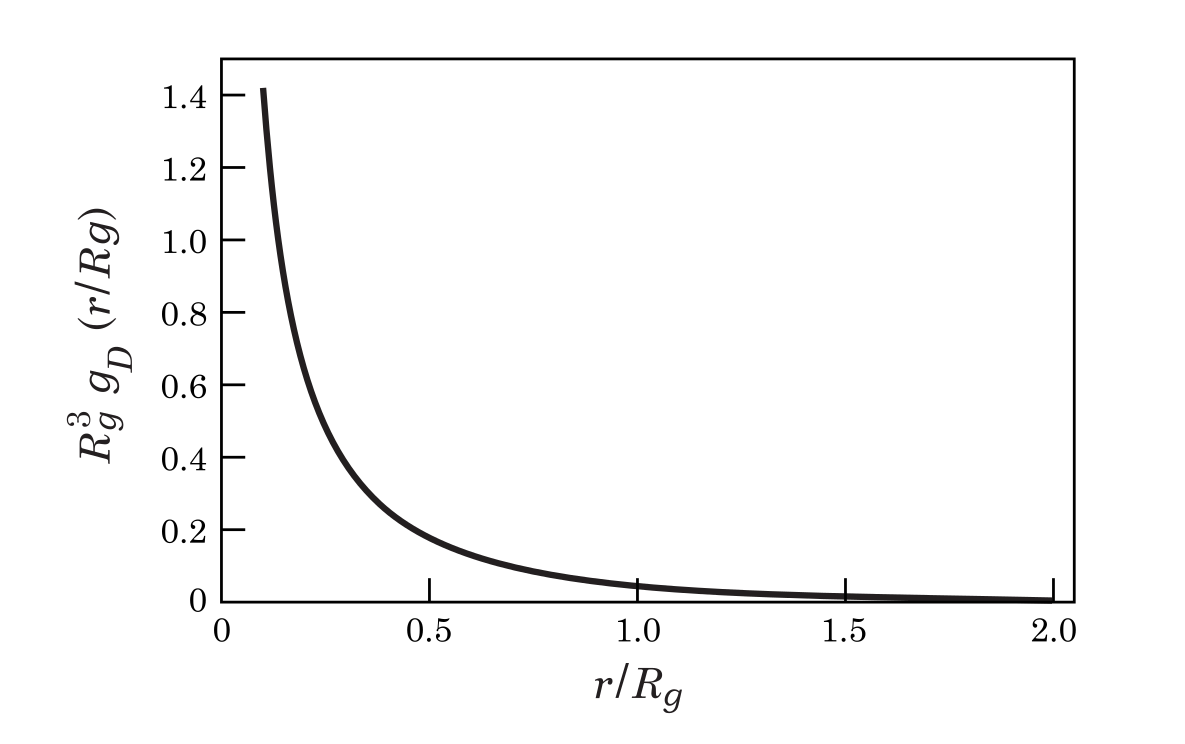
\includegraphics[scale=0.4]{Contents/chapter3/figures/FIG3-9.png}
	\caption{由(\ref{3.113})定义的Debye函数逆傅里叶变换,并以$\frac{r}{R_g}$为横坐标,以${R_g}^3 g_D(r)$为纵坐标.}
	\label{FIG3.9}
\end{figure}

形如(\ref{FIG3.9}),$\frac{r}{R_g} \ll 1$时,函数以$\frac{1}{r}$的速度代数衰减:
\begin{equation}
g_D(r) \sim \frac{3}{\pi b^2 N r}
\end{equation}
$r \sim R_g$时,函数单调的指数级的衰减为零:
$$g_D(r) \sim \frac{1}{r} e^{-\frac{\sqrt{3}r}{R_g}}$$

将弱非均匀性展开应用到其他聚合物体系(包括支链聚合物,共聚物)是非常直接的.

例如,在三臂星形均聚物的情况下,臂长相等,即$N_j = N$,
则
\begin{equation}
Q[w] = \frac{1}{V} \int [q(\br ,N;[w])]^3\,\mathrm{d} \br 
\end{equation}
又由(\ref{3.116})和(\ref{3.119})可得
\begin{equation}
Q[w] \sim e^{-3w_0 N} [1+\frac{3 {\epsilon_a}^2 N^2}{2V^2} \sum_{\mathbf{k}} \hat{g_S}(k^2 {R_g}^2)\hat{\omega}(\mathbf{k})\hat{\omega}(-\mathbf{k})+\dots]
\end{equation}
其中${R_g}^2 = \frac{Nb^2}{6}$为星形中一臂的旋转半径,$g_S(x)$为类Debye函数
\begin{equation}
\hat{g_S}(x) = \hat{g_D}(x) + 2[\hat{h_D}(x)]^2
\end{equation}
其中
\begin{equation}
\hat{h_D}(x) = \frac{1}{x} [1-e^{-x}]
\end{equation}
从而密度算子和对相关函数分别为
\begin{equation}
\rho(\br ;[w]) \sim \rho_0[1-\epsilon_a N \int g_S(|\br -\br ') \omega(\br ')\,\mathrm{d} \br '+O({\epsilon_a}^2)]
\end{equation}




\chapter{多链系统模型}
 {\color{red}\begin{center}
      邱群  
    \end{center}}
   
前两章主要讨论了在孤立情况和外部势场作用下聚合物单链的统计性质.
    在这里我们将讨论在溶液中和熔融状态下多条相互作用聚合物链更真实的情况,
    而一直被忽略的分子内的长程作用力也将包含在公式中(formalism).
    \section{从粒子到场}
    正如第一章所讨论的那样,
    基于场方法模拟非均匀聚合物的一个基本的原理就是将基于粒子的模型转换为统计场理论.
    本章一个重要的目标就是说明如何对庞大的聚合物和复杂流体体系进行粒子到场的变换.
    这一般的方法就是使用一个与Hubbard-Stratonovich变换有关的有效技术(formal
    technique),
    这种技术可用粒子与一个或多个辅助场之间的相互作用来代替具有解耦作用的粒子(或聚合物段)间的相互作用.
    我们可以看到这些场与上一章我们讨论的外场发挥了相同的作用,
    尽管它们是流体内部产生的. 本章描述的方法是在凝聚态(Chakin and Lubensky,
    1995), 经典液态(Caillol, 2003), 以及聚合物物理共同体(Edwards, 1996;
    Helfend, 1975; Hong and Noolandi, 1981 )中比较熟知的.
    然而只是最近才有场理论是软凝聚态物质体系是计算机模拟的基础的结论.
    \par
    无论是从流体的原子的还是介观的原始模型粒子到场的变换都是可做的.
    我们可以从单原子流体最简单的情况开始比如氩. 
%\par
 %   前两章主要讨论了在孤立情况和外部势场作用下聚合物单链的统计性质\.在此我们将讨论在溶液中和熔融状态下多条相互作用聚合物更现实的情况\.这需要处理属于不同聚合物链段之间的相互作用\,而一直被忽略的分子内的长程作用力也将包含在形式体系上(formalism)\.
  %  \subsecton
    \subsection{正则系综下的单原子流体}
    在正则系综中, 一个体系被认为是对物质交换是封闭的, 但对能量交换是开放的,
    它通过与一个在固定温度$T$下的热源交换热量. 一个具有$n$个不同原子限制在体积为$V$上的经典的单原子流体的正则配分函数可以表示成(Chandler,
    1987)
\label{subsec.equations}
    \begin{equation}
        \begin{aligned}
            Z_C(n, V, T)=\frac{1}{n!\lambda_T^{3n}}\int d\bm{r}^n
            \exp[-\beta U(\bm{r}^n)].
        \end{aligned}
        \label{eq.1}
    \end{equation}
其中$\lambda_T=\frac{h}{\sqrt{2\pi mk_BT}}$是热波长, $m$是原子质量,
$h$是Planck常数. 势能$U(\bm{r}^n)$依赖于$n$个原子的位置关系,
通过确定它的数学形式可以定义一个流体的特殊的原子模型.
通常情况下式(1.2)是対势能的准确描述. 为了便于说明, 我们将采用这种观点,
并写成\\
\label{subsec.equations}
   \begin{equation}
       \begin{aligned}
           U(\bm{r}^n)=\frac{1}{2}\sum_{j=1}^n \sum_{k=1(\neq j)}^n
           u(|\bm{r}_j-\bm{r}_k|).
       \end{aligned}
       \label{eq.2}
    \end{equation}
其中$u(r)$是我们熟悉的対势函数(Hansen and McDnald,
1986).表达式中的因子$\frac{1}{2}$纠正了在求和时每个粒子的対势函数重复算了两次的误差.
就氩而言,
式(1.3)给出的Lennard-Jones势为适合$u(r)$量子化学的计算提供了一个合理的两参数法.
更一般的, 这也可以用来处理一大类原子流体, 甚至某些分子流体(比如甲烷),
它们可以通过保持$u(r)$形式的任意性, 用球对称対势函数来描述.
\par
影响粒子到场变换的对$u(r)$一个必要的限制就是接触势(on
contact)必须是有限的, 即$|u(0)|<\infty$. 这似乎排除了比如许多重要的势函数,
包括Lennard-Jones势和硬核势(the hard sphere potential),
而实际上, 在不影响流体结构和热动力学的情况下,
将这样的势正则化使$|u(0)|$有限是很简单的.
比如说Lennard-Jones势可以通过一个简单的位移$\delta$正则化, 根据
\label{subsec.equations}
   \begin{equation}
       \begin{aligned}
           u(r)=4\epsilon\{ [\frac{(r+\delta)}{\sigma}]^{-12}-
           [\frac{(r+\delta)}{\sigma}]^{-6} \}.
      \end{aligned}
       \label{eq.3}
    \end{equation}
选$\delta=0.01\sigma$会得到$u(0)=4\times10^{24}$,
这个数如此之大以至于重叠的粒子结构不会给$Z_C$提供可视的贡献, 因此没有热力学作用.
同样地, 在不影响流体的热力学性质的情况下, 也可以将一个硬球势正则化, 
通过用一个有限但非常大的势阶跃来代替在硬核直径$r=\sigma$处无限势阶跃.
下面,我们假设$u(r)$都可以通过这样的方式正则化.
\par
接下来的任务就是用微观密度算子(microscopic density
operator)来改写(\ref{eq.2}). 通过类比式(3.3),
我们将微观粒子密度定义为集中在每个原子坐标的狄拉克$\delta$函数的总和
\label{subsec.equations}
   \begin{equation}
       \begin{aligned}
           \hat{\rho}(\bm{r})=\sum_{j=1}^{n} \delta(\bm{r}-\bm{r}_j).
     \end{aligned}
       \label{eq.4}
    \end{equation}
由此可见
\label{subsec.equations}
   \begin{equation}
       \begin{aligned}
         U(\bm{r}^n)=\frac{1}{2} \int d\bm{r} \int
           d\bm{r^{'}}\hat{\rho}(\bm{r})u(|\bm{r}-\bm{r^{'}}|)\hat{\rho}(\bm{r^{'}})-\frac{1}{2}nu(0).
     \end{aligned}
       \label{eq.5}
    \end{equation}
其中最后一项扣除了包含在第一项中n个原子的自身相互作用.
因此(\ref{eq.1})可以被写成
\label{subsec.equations}
   \begin{equation}
       \begin{aligned}
           Z_C=\frac{z_0^n}{n!} \int d\bm{r}^n \exp \big( -\frac{\beta}{2}\int d\bm{r}\int
           d\bm{r^{'}}\hat{\rho}(\bm{r})u(|\bm{r}-\bm{r^{'}}|)\hat{\rho}(\bm{r^{'}})
           \big).
     \end{aligned}
       \label{eq.6}
    \end{equation}
其中$z_0=\exp(\beta u(0)/2)/{\lambda_T^3}$.
从这个结果可以看到在初始点势能的值$u(0)$,
它只影响流体的化学势而没有任何热力学后果.
\par
场到粒子的变换的下一步就是利用$\delta$泛函的定义, 即
\label{subsec.equations}
   \begin{equation}
       \begin{aligned}
           \int D\rho\ \delta[\rho-\hat{\rho}]F[\rho]=F[\hat{\rho}].
         \end{aligned}
       \label{eq.7}
    \end{equation}
$F[\rho]$为任意泛函.
$\delta$函数可以看做是,
在定义域的所有我们所关心的点处,除非$\rho(\bm{r})$和$\hat{\rho(\bm{r})}$相等,
否则其值为0的一个无限维的狄拉克$\delta$函数.
一个非常有用的$delta$函数的复指数表达式通过用$M_g$离散空间可以演变成
\label{subsec.equations}
   \begin{equation}
       \begin{aligned}
           \delta[\rho-\hat{\rho}] &\approx\prod_{\bm{r}} \delta(\rho(\bm{r})-\hat{\rho}(\bm{r}))
           \\&=\frac{1}{(2\pi)^{M_g}}\prod_{\bm{r}}\left\{
               \int_{-\infty}^{\infty}
               d\omega(\bm{r})e^{i\omega(\bm{r})[\rho(\bm{r})-\hat{\rho}(\bm{r})]}
               \right\}
           \\&=\int D\omega\ e^{i\int\ d\bm{r}\ 
           \omega(\bm{r})[\rho(\bm{r})-\hat{\rho(\bm{r})}]}.
         \end{aligned}
       \label{eq.8}
    \end{equation}
上述表达式的第二行是根据等式(A.15)的应用得出来的,
其中(A.15)表示在网格点$\bm{r}$处一维的$\delta$函数$\delta(\rho(\bm{r})-\hat{\rho}(\bm{r}))$.
前置因子$\frac{1}{(2\pi)^{M_g}}$包含了所有网格点的归一化因子.
(\ref{eq.8})最后一个表达式是连续的描述,
而且可以看作是关于辅助场$\omega(\bm{r})$泛函积分$\int D\omega$正式的定义.
非常重要的是要注意到$\omega(\bm{r})$是一个标量场,
而且(\ref{eq.8})中的泛函积分在每个$\bm{r}$处沿着整个实轴进行.
\par
将正则配分函数转换成统计场理论的下一步是将$F[\rho]=1$时的(\ref{eq.7})插入(\ref{eq.6})的被积函数中,
这将会推出
\label{subsec.equations}
   \begin{equation}
       \begin{aligned}
           Z_C=\frac{z_0^n}{n!} \int D\rho \int d\bm{r}^n \delta[\rho-\hat{\rho}] \exp \big( -\frac{\beta}{2}\int d\bm{r}\int
           d\bm{r^{'}}\rho(\bm{r})u(|\bm{r}-\bm{r^{'}}|)\rho(\bm{r^{'}})
           \big).
     \end{aligned}
       \label{eq.9}
    \end{equation}
其中我们用到了任意一个泛函$G[\rho]$的$\delta$函数的以下性质:
$\delta[\rho-\hat{\rho}]G[\hat{\rho}]=\delta[\rho-\hat{\rho}]G[\rho]$.
接下来将(\ref{eq.8})作为$\delta$函数插入, 结果表达式将会变成
\label{subsec.equations}
   \begin{equation}
       \begin{aligned}
           Z_C=\frac{z_0^n}{n!} \int D\rho \int D\omega \int d\bm{r}^n
           e^{i\int d\bm{r}\omega(\rho-\hat{\rho}) -\frac{\beta}{2}\int d\bm{r}\int
           d\bm{r^{'}}\rho u\rho}.
     \end{aligned}
       \label{eq.10}
    \end{equation}
\par
非常重要地是要注意, 经过这些变换,
$\exp(-i\int d\bm{r} \omega
\hat{\rho})$是被积函数中唯一依赖于原子坐标$\bm{r}^n=(\bm{r}_1,\ldots,\bm{r}_n)$的因子.
积分在n个粒子位置上的因式分解是
\label{subsec.equations}
   \begin{equation}
       \begin{aligned}
           \int d\bm{r}^n e^{-i\int d\bm{r} \omega \hat{\rho}}&=\int d\bm{r}^n
           e^{-i\sum_{j=1}^n \omega(\bm{r}_j)}
           \\&=\prod_{j=1}^n \left\{ \int_V d\bm{r}_j e^{-i\omega(\bm{r}_j)}
           \right\}=(VQ[i\omega])^n.
    \end{aligned}
       \label{eq.11}
    \end{equation}
其中
\label{subsec.equations}
   \begin{equation}
       \begin{aligned}
           Q[i\omega]\equiv \frac{1}{V}\int_V d\bm{r} e^{-i\omega(\bm{r})}
    \end{aligned}
       \label{eq.12}
    \end{equation}
泛函$Q[i\omega]$可以解释为单粒子配分函数,
即一个不与其它原子相互作用,
而仅仅只与一个纯虚场$\omega{\b{r}}$相互作用的原子对配分函数的贡献.
正如第三章所讨论的, 单原子配分函数也有相同的解说和归一化$Q[0]=1$, 
因此我们采用相同的符号Q. 显而易见, $Q[i\omega]$是一个原子的局部泛函,
然而对于一个聚合物分子来说, 它是一个高度非局部泛函. 因此,
相比于聚合物,计算原子的$Q[i\omega]$要简单得多.
\par
将(\ref{eq.10})和(\ref{eq.11})联合起来, 粒子到场的变换就完成了.
配分函数可以表达成下面的统计场理论:
\label{subsec.equations}
   \begin{equation}
       \begin{aligned}
          Z_C=(n, V, T)=Z_0\int D\rho \int D\omega \exp(-H[\rho, \omega]).
    \end{aligned}
       \label{eq.13}
    \end{equation}
其中泛函
\label{subsec.equations}
   \begin{equation}
       \begin{aligned}
           H[\rho, \omega]=-i\int d\bm{r}\ 
           \omega(\bm{r})\rho(\bm{r})+\frac{\beta}{2}\int d\bm{r} \int
           d\bm{r^{'}} \rho(\bm{r})u(|\bm{r}-\bm{r^{'}}|)\rho(\bm{r^{'}})-n\ln
           Q[i\omega].
    \end{aligned}
       \label{eq.14}
    \end{equation}
被称为"有效哈密顿量"或者"作用"(Pairsi, 1988; Zee,2003).
(\ref{eq.13})中前置因子: $Z_0\equiv(z_0V)^{n}/{n!}$与理想气体的配分函数成正比.
\par
(\ref{eq.13})是本节的中心结论,
即可用任意対势函数描述成对相互作用的单原子流体的配分函数可以表示成统计场论.
配分函数已被证明它是与一个类似波尔曼因子: $\exp(-H[\rho,
\omega])$关于两个波动场(fluctuating field)$\rho(\bm{r})$和$\omega(\bm{r})$的泛函成正比的.
第一个场$\rho$可以被解释为波动粒子数密度,
因为它限制了在(\ref{eq.9})中引入的$\hat{\rho}$.
第二个场$\omega(\bm{r})$可以被看做是波动非均匀化学场,
因为它作为有效哈密顿量H的第一项中的场$\rho$的共轭变量出现.
$\omega(\bm{r})$与流体的平衡化学式$\mu$之间的对应关系在4.1.3节将更为精确.
\par
\ref{eq.14}表明具有自由能泛函特点的有效哈密顿量有三个主要的贡献. 第一项:$-i\int
d\bm{r}$可以被解释为密度场$\rho$与纯虚场相互作用的能量. 第二项与$\int d\bm{r}
\int d\bm{r^{'}} \rho u \rho$成比例, 表示与粒子间相互作用的能量.
最后是, 项$-n\ln
Q[i\omega]$表示在$i\omega(\bm{r})$势下具有n个不相互作用的流体的平移熵(相对于理想气体熵).
虽然$H[\rho, \omega]$有焓和熵的贡献也有自由能特性,
但是它不同于流体的Helmhohlz自由能A, 因为后者包括了与波动场$\rho$和$\omega$有关的熵贡献.
事实上Helmholz自由能的计算包含了熟悉的热力学关联公式的使用
\label{subsec.equations}
   \begin{equation}
       \begin{aligned}
           A(n, V, T)=-k_BT \ln Z_C(, V, T).
       \end{aligned}
       \label{eq.15}
    \end{equation}
其中$Z_C$是通过(\ref{eq.13})对场$\rho$和$\omega$进行泛函积分得到的.
\par
非常明显地可以看到,
化学势场$\omega$是在支持单个原子与纯虚场$i\omega$相互作用的情况下, 原子间解耦相互作用结果.
这个场是内部作用的结果, 但从计算单粒子配分函数的角度看, 它可以看作是外部施加的.
因此可以将$\omega$看作是上一章中的外部场.
\par
在实理论中出现纯虚数, 咋一看也许会感到惊讶,
因为配分函数$Z_C$是实的,正如场$\rho$和势函数$\mu$一样.
有效哈密顿量$H$很明显是复的而且可以分解成实部和虚部$H_R+iH_I$.
一个非常重要的结论就是:
在(\ref{eq.14})被积函数中类似于玻尔兹曼因子的$\exp(-H)$包含了一个复相因子$\exp(-iH_I)$,
它根据$\rho$和$\omega$的结构而回出现符号振荡.
因此定义配分函数的的泛函积分包含了一个振荡的被积函数. 这个特点将会在第六章看到,
在模拟像这样的场理论时会产生困难(称为"符号问题"), 这会要求特殊的数值技术.
\par
有人可能会问是否真的需要进行一个复的泛函积分才能得到一个实的配分函数,
事实上,我们可以利用$Z_C$是实的这一事实,
我们可以在原始等式上加上(\ref{eq.13})的复共轭, 可得到
\label{subsec.equations}
   \begin{equation}
       \begin{aligned}
           Z_C(n, V, T)=Z_0 \int D\rho \int D\omega \exp(-H_R[\rho, \omega])
           \cos(H_I[\rho, \omega]).
        \end{aligned}
       \label{eq.16}
    \end{equation}
因此被积函数显然是实的. 然而由于相因子$\cos(H_I)$不是正定的,
所以被积函数仍然是振荡的.
因此如果我们希望将粒子语言转换成场语言, 符号问题是不可避免的,
其中粒子语言中统计质量$\exp(-\beta U)$是正定的,
但在场理论中对应的量$\exp(-H)$却不是. 尽管如此,
但场理论描述的优势一般来说还是大于由非正定性带来的困难的,
至少对于相对浓缩的聚合物熔体和溶液是这样的.
下面将证明用(\ref{eq.13})给出的复场理论比(\ref{eq.16})给出的场理论要更方便,
当然, 它们是等价的.
\par
(\ref{eq.13})-(\ref{eq.14})定义了一个包含两个场的场论,
该场论适用于带有任意(但正则化的)対势函数$u(r)$的单原子流体. 对某些特殊的势函数,
即从
\label{subsec.equations}
   \begin{equation}
       \begin{aligned}
           \int d\bm{r^{'}} u(|\bm{r}-\bm{r^{'}}|)
           u^{-1}(|\bm{r^{'}}-\bm{r^{''}}|).
       \end{aligned}
       \label{eq.17}
    \end{equation}
意义上来说是可逆的, 且$u(|\bm{r}-\bm{r^{'}}|)$是正定的. 特别地,
如果这些都满足了, 那么$\ref{eq.13}$是式(C.28)形式的高斯积分且可以进行解析计算.
如果$u$的傅里叶变换
\label{subsec.equations}
   \begin{equation}
       \begin{aligned}
           \hat{u}(\bm{k})=\int d\bm{r}\ u(r)\exp(-i\bm{k\cdot
           r})=4\pi\int_0^{\infty} dr\ r^2 j_0(kr)u(r).         
       \end{aligned}
       \label{eq.18}
    \end{equation}
存在且是对所有的$k=|\bm{k}|$都是正的话,
则u满足正定和可逆的双重条件. 对于这样的势, (\ref{eq.13})可以简化成
\label{subsec.equations}
   \begin{equation}
       \begin{aligned}
       Z_C(n, V, T)=Z_0\int D\omega \exp(-H(\omega)).
       \end{aligned}
       \label{eq.19}
    \end{equation}
其中一个场独立的归一化因子已被吸收到关于$\omega$的泛函积分的定义中去了.
新的有效的哈密顿量只依赖于单个场$\omega$
\label{subsec.equations}
   \begin{equation}
       \begin{aligned}
           H[\omega]=\frac{1}{2\beta}\int d\bm{r} \int d\bm{r^{'}}\
           \omega(\bm{r}) u^{-1}(|\bm{r}-\bm{r^{'}}|)\omega(\bm{r^{'}}) -n\ln
           Q[i\omega]
       \end{aligned}
       \label{eq.20}
    \end{equation}
粒子与粒子间的相互作用包含在了这个哈密顿量的第一项中, 而且哈密顿量还包含了对势函数的逆.
\par
应用(\ref{eq.19})-(\ref{eq.20})简化描述的対势的重要粒子包括单参数排斥性$\delta$函数势
\label{subsec.equations}
   \begin{equation}
       \begin{aligned}
           u(r)=u_0\delta(\bm{r})
       \end{aligned}
       \label{eq.21}
    \end{equation}
其中$u_0 >0 $, 而且排斥Yukawa(或Debye-H$\ddot{u}$ckel)势
\label{subsec.equations}
   \begin{equation}
       \begin{aligned}
           u(r)=\frac{u_0}{4\pi r}\exp(-kr).
       \end{aligned}
       \label{eq.22}
    \end{equation}
其中$u_0>0, k\geq 0$. 当$k=0$时,后者会产生排斥库伦势.
这些势在$r=0$处是没有正则化的,但是这个是很容易做到的. 例如, 排斥阶跃势
\label{subsec.equations}
   \begin{equation}
       u(r)=\left\{
       \begin{aligned}
           3u_0/(4\pi\delta^3),& &\ 0\leq r\leq\delta
               \\
           0,& &\ r>\delta
       \end{aligned}
       \right.
       \label{eq.23}      
    \end{equation}
在$u_0, \delta>0$时, 当$\delta\longrightarrow 0_{+}$,
它与$\delta$函数势(\ref{eq.21})有相同的傅里叶变换,但是在初始点是有限的.
对于非常小的但不为零的$\delta$,
\ref{eq.23}表示的势也满足非负性和正则性的法则[波数$k\lesssim O(1/\delta)$].
\par
不幸的是,大多数具有硬核的实际对势不满足(\ref{eq.19})-(\ref{eq.20})适用的条件,
比如(\ref{eq.3})的正则Lennard-Jones势. 在这样的情况下,
必须使用等式(\ref{eq.13})-(\ref{eq.14})的全场理论. 从全理论的推导可以看出,
为解耦相互作用提出的方法并不局限于对可分解的势函数,
事实上,当模型中$U(\bm{r})$存在三体相互作用时场到粒子的变换也是可以进行的.
尽管像这样的相互作用不能简化成只包含单个$\omega$场的场理论.

\subsection{巨正则系综中的单原子流体}
解耦技术可推广用于推导其它重要系综的统计场理论.例如,
用对物质交换和能量交换都是开放的巨正则系综来研究流体体系的统计热力学是非常方便(Chandler,
1987; McQuarrie, 1976; Hansen and McDonald, 1986).
相关的巨正则系综的配分函数可以写成
\label{subsec.equations}
   \begin{equation}
       \begin{aligned}
           Z_G(\mu, V ,T)=\sum_{0}^{\infty} \exp(\beta\mu n)Z_C(n, V,T).
       \end{aligned}
       \label{eq.24}      
    \end{equation}
其中$\mu$是化学势且是对所有的原子数求和.
将(\ref{eq.10})-(\ref{eq.11})插入表达式的右端, 则立即得
\label{subsec.equations}
   \begin{equation}
       \begin{aligned}
           Z_G=\int D\rho \int D\omega\ e^{i\int d\bm{r}\ 
           \omega\rho-(\beta/2)\int d\bm{r} \int d\bm{r{'}} \rho u
           \rho}\sum_{n=0}^{\infty}\frac{(zVQ[i\omega])^n}{n!}.
       \end{aligned}
       \label{eq.25}      
    \end{equation}
其中$z\equiv z_0\exp(\beta u)$是一个活跃量(the activity).
对关于粒子数的求和的估计推出了巨正则系综的理想场论:
\label{subsec.equations}
   \begin{equation}
       \begin{aligned}
           Z_G(\mu, V ,T)=\int D\rho \int D\omega \exp(-H_G[\rho, \omega]).
       \end{aligned}
       \label{eq.26}      
    \end{equation}
其中
\label{subsec.equations}
   \begin{equation}
       \begin{aligned}
           H_G[\rho, \omega]=-i\int
           d\bm{r}\omega(\bm{r})\rho{\bm{r}}+\frac{\beta}{2}\int d\bm{r}
           \int d\bm{r^{'}}\ \rho(\bm{r}) u(|\bm{r}-\bm{r^{'}}|)
           \rho(\bm{r^{'}})-zVQ[i\omega].
       \end{aligned}
       \label{eq.27}      
    \end{equation}
在这个系综中的热力学联系是通过状态方程
\label{subsec.equations}
   \begin{equation}
       \begin{aligned}
           pV=k_B T\ln Z_G(\mu, V, T).
       \end{aligned}
       \label{eq.28}      
    \end{equation}
得到的, 其中$p$是压力, 且根据
\label{subsec.equations}
   \begin{equation}
       \begin{aligned}
           \langle n \rangle=\left(\frac{\partial \ln Z_G(\mu, V, T)}{\partial \ln z}
           \right)_{V, T}.
       \end{aligned}
       \label{eq.29}      
    \end{equation}
可通过调节化学势$\mu$和活跃量$z$来控制平均粒子数.
\par
比较正则系综和巨正则系综的有效哈密顿量(\ref{eq.14})和$\ref{eq.27}$,
我们可以看到它们唯一的区别在于最后一项平移熵的形式不同,
因此我们可以直接在场理论的框架中切换系综. 最后,
如果$u(r)$正如前一节描述的那样是正定且可逆的,
那么巨正则系综同样地也可以简化成只包含场$\omega$的统计场理论:
\label{subsec.equations}
   \begin{equation}
       \begin{aligned}
           Z_G(\mu, V ,T)=\int D\omega \exp(-H_G[\omega]).
       \end{aligned}
       \label{eq.30}      
    \end{equation}
其中有效哈密顿量为
\label{subsec.equations}
   \begin{equation}
       \begin{aligned}
           H_G[\omega]=\frac{1}{2\beta}\int d\bm{r}
           \int\bm{r^{'}}\omega(\bm{r})u^{-1}(|\bm{r}-\bm{r^{'}}|)\omega(\bm{r^{'}})-zVQ[i\omega].
       \end{aligned}
       \label{eq.31}      
    \end{equation}
再一次(\ref{eq.20})与(\ref{eq.31})唯一的区别在于平移熵项.

\subsection{单原子流体的平均和运算符}
已经证明了如何将基于原子的粒子模型转换成场理论,
现在比较适合来讨论我们所关心的系综平均量是如何计算的.
对某些任意可视量$G[\rho, \omega]$,
其可以表示成波动场量$\rho$和$\omega$的泛函的形式, $G$的系综平均可以定义成
\label{subsec.equations}
   \begin{equation}
       \begin{aligned}
           \langle G[\rho, \omega] \rangle=\frac{\int D\rho \int D\omega G[\rho,
           \omega] \exp(-H[\rho, \omega])}{\int D\rho \int D\omega
           \exp(-H[\rho, \omega])}.
       \end{aligned}
       \label{eq.32}      
    \end{equation}
在正则系综中这个表达式非常适用与使用全场理论来计算平均值.
相应的巨正则系综的平均可用$H_G[\rho, \omega]$替换$H[\rho, \omega]$来定义.
当対势是可逆的且(\ref{eq.19})-(\ref{eq.20})或者(\ref{eq.30})-(\ref{eq.31})的简单理论适用的情况下,
可视量$G[\omega]$的平均可定义为
\label{subsec.equations}
   \begin{equation}
       \begin{aligned}
           \langle G[\omega] \rangle=\frac{\int D\omega G[\omega] \exp(-H[\omega])}{\int D\omega
           \exp(-H[\omega])}.
       \end{aligned}
       \label{eq.33}      
    \end{equation}
其中在巨正则系综中用$H_G[\omega]$来代替$H[\omega]$也是很好理解的.
\par
在正则系综中一个非常重要的热力学量就是通过$\mu=(\partial A/\partial n)_{T,
V}$定义的化学式, 它来自(\ref{eq.13})-(\ref{eq.15})
\label{subsec.equations}
   \begin{equation}
       \begin{aligned}
           \mu=\mu_0-k_BT \langle \ln Q[i\omega] \rangle.
       \end{aligned}
       \label{eq.34}      
    \end{equation}
其中$\mu_0=k_B T(\partial \ln Z_0/\partial n)_{T, V}$是理想气体的化学式.
这个表达式表明, 化学势的额外贡献是由关于波动场的运算符$-k_BT\ln
Q[i\omega]$的平均值给出的. 对$\omega$通常的认识就是,
这个运算符既有实部也有复部, 但是它的虚部平均值为零, 只留下化学势的纯实部.
\par
在巨正则系综中, 一个紧密相关的热力学量是平均粒子密度,定义为$\rho_0\equiv
\langle n \rangle\/V$, $V$是(\ref{eq.29})给出的. 通过式中所示倒数可以看到,
根据$\langle n \rangle=zV\langle Q[i\omega] \rangle$, 因此
\label{subsec.equations}
   \begin{equation}
       \begin{aligned}
           \rho_0 \equiv \frac{\langle n \rangle}{V}=z\langle \ln Q[i\omega] \rangle.
       \end{aligned}
       \label{eq.35}      
    \end{equation}
因此$zQ[i\omega]$可以看作是一个运算符,
其平均在巨正则系综中关于$\omega$场波动求平均会推出平均粒子密度.
\par
另一个重要的系综平均的类是与粒子密度相关函数有关的.
在包含$\rho$和$\omega$场的全理论中,
密度相关函数可以直接用关于$\rho$合适的因子的平均来计算. 例如,
在正则系综中密度-密度相关函数$\langle
\rho(\bm{r})\rho(\bm{r^{'}})\rangle$的计算可以通过
\label{subsec.equations}
   \begin{equation}
       \begin{aligned}
           \langle \rho(\bm{r})\rho(\bm{r^{'}})\rangle=\frac{\int D\rho \int
           D\omega \rho(\bm{r})\rho(\bm{r^{'}})\exp(-H[\rho, \omega])}{\int D\rho \int D\omega
           \exp(-H[\rho, \omega])}.
       \end{aligned}
       \label{eq.36}      
    \end{equation}
这个量与简单流体中的$X$射线和中子散射实验中的散射辐射强度有关(Hansen and
McDonald, 1986). 相似地, 在巨正则系综中原子平均局部密度可以通过
\label{subsec.equations}
   \begin{equation}
       \begin{aligned}
           \langle \rho(\bm{r})\rangle=\frac{\int D\rho \int
           D\omega \rho(\bm{r})\exp(-H[\rho, \omega])}{\int D\rho \int D\omega
           \exp(-H[\rho, \omega])}.
       \end{aligned}
       \label{eq.37}      
    \end{equation}
给出.
\par
在巨正则系综中$\rho(\bm{r})$的另一种推导是具有指导意义的.
注意到(\ref{eq.37})可以重新表示成
\label{subsec.equations}
   \begin{equation}
       \begin{aligned}
          \langle \rho(\bm{r}) \rangle=\frac{1}{Z_G} \int D\rho \int D\omega\
           e^{zVQ[i\omega]-(\beta/2)\int d\bm{r}\int d\bm{r^{'}}\rho u\rho}
           \frac{\delta}{i\delta\omega(\bm{r})} e^{i\int d\bm{r}\ \omega\rho}.
       \end{aligned}
       \label{eq.38}      
    \end{equation}
假设当$\omega(\bm{r})\longrightarrow\pm\infty$时, $\int D\rho
\exp{-H_G}$衰退为0对值域中所有的点$\bm{r}$都成立, 通过分部积分将会推出
\label{subsec.equations}
   \begin{equation}
       \begin{aligned}
           \langle \rho(\bm{r}) \rangle&=-\frac{1}{iZ_G} \int D\rho \int D\omega\
           e^{\int d\bm{r} \omega\rho(\beta/2)\int d\bm{r}\int d\bm{r^{'}}\rho u\rho}
           \frac{\delta}{\delta\omega(\bm{r})} e^{zVQ[i\omega]}
           \\
           &=\langle izV\frac{\delta Q[i\omega]}{\delta\omega(\bm{r})}
           \rangle=\langle z\exp[-i\omega(\bm{r})] \rangle.
       \end{aligned}
       \label{eq.39}      
    \end{equation}
其中在推导的最后一个表达式中,
我们使用了(\ref{eq.12})给出的单粒子配分函数的显示形式. 最后一个表达式表明,
在巨正则系综中运算符$\rho{\bm{r}}$的平均是和$z\exp[-i\omega(\bm{r})]$是等价的.
进一步, 对(\ref{eq.39})两边求体积平均会推出(\ref{eq.35}), 与预期的
\label{subsec.equations}
   \begin{equation}
       \begin{aligned}
           \rho_0=\frac{1}{V}\int d\bm{r}\langle \rho(r) \rangle.
       \end{aligned}
       \label{eq.40}      
    \end{equation}
是保持一致的.
\par
另外一个我们感兴趣的热力学量是压力$p$.
在巨正则系综中, 当$Z_G$可以被计算时, 压力可通过(\ref{eq.28})直接计算出来.
在正则系综的场理论框架中, 压力是一个更不可估摸的量.
一种对不同的对势$u(r)$都适用的方法是通过$Z_C$的粒子表达式推导出来的(Chandler,
1987; McQuarrie, 1986)
\label{subsec.equations}
   \begin{equation}
       \begin{aligned}
           \beta p/\rho_0=1-\frac{\beta}{6n} \sum_{j=1}^{n} \sum_{k=1(\neq j)}^{n} \langle v(|\bm{r_j}-\bm{r_k} |)\rangle.
       \end{aligned}
       \label{eq.41}      
    \end{equation}
在这个表达式中, $\rho=n/V$是正则系综中的平均密度, $v(r)=rdu(r)/dr$是维里函数.
(\ref{eq.41})可以重写成带有关于微观粒子密度平均的项,
反过来也可以用场理论描述中的$\rho$场的平均来代替:
\label{subsec.equations}
   \begin{equation}
       \begin{aligned}
           \beta p\rho_0=1-\frac{\beta}{6n} \int d\bm{r} \int d\bm{r^{'}}
           v(|\bm{r}-\bm{r^{'}} |) [\langle \rho(\bm{r})\rho(\bm{r^{'}})
           \rangle -\delta(\bm{r}-\bm{r^{'}})\langle\rho(\bm{r})\rangle ].
       \end{aligned}
       \label{eq.42}      
    \end{equation}

%文章引用\,\cite{,}.
%\subsection{方程}
%\label{subsec.equations}
%\begin{itemize}
%	\item[$\bullet$] 示例 1
%	\begin{equation}
%		\begin{aligned}
%			a = b,
%			\\
%			b = c.
%		\end{aligned}
%		\label{eq.1}
%	\end{equation}
%	\item[$\bullet$] 示例 2
%	\begin{equation}
%		\left\{
%		\begin{aligned}
%			a = b,
%			\\
%			b = c.
%		\end{aligned}
%		\right.
%		\label{eq.2}
%	\end{equation}
%\end{itemize}
%
%
%\subsection{表格}
%\label{subsec.table}
%%% A, a, I, i, 1
%%% \Alph, \alph, \Roman, \roman, \arabic
%\begin{enumerate}[(I)]
%	\item 示例 1
%	\begin{table}[htbp]
%		\centering
%		\caption{表格示例}
%		\label{tab.1}
%		%% set the width of each column;
%		\begin{tabular}{p{3.5cm}|p{2cm}|p{5cm}<{\centering}}
%			\hline
%			a &b &c\\
%			\hline
%		\end{tabular}
%	\end{table}
%\end{enumerate}
%
%
%\subsection{图像}
%\label{subsec.figure}
%\begin{figure}[htbp]
%    \centering
%    \begin{minipage}[t]{0.2\linewidth}
%%        \centerline{\includegraphics[scale=0.4]{figure/figure1.png}}
%        \footnotesize{\centerline{(a)}}
%    \end{minipage}
%    \hspace{0.2\linewidth}
%    \begin{minipage}[t]{0.2\linewidth}
%%        \centerline{\includegraphics[scale=0.4]{figure/figure2.png}}
%        \footnotesize{\centerline{(b)}}
%    \end{minipage}
%    \caption{图像示例}
%	\label{fig.1}
%\end{figure}
%


%\section*{致谢} 

%%% 附录;
%    \newpage
%\begin{appendix}
    \section{附录}
    公式的推导.
    \par
    \textbf{公式(\ref{eq.8})}
    \\
    由书上附录(A.15)($P_{389}$)$\delta$函数的定义
\label{subsec.equations}
    \begin{equation}
        \begin{aligned}
            \delta(x)=\frac{1}{2\pi}\int^{+\infty}_{-\infty}dk\ \exp(ikx)
        \end{aligned}
        \label{A.1}
    \end{equation}
    \par
    \textbf{公式(\ref{eq.9})} 
    \\
    由(\ref{eq.7}):
\label{subsec.equations}
   \begin{equation}
       \begin{aligned}
           \int D\rho\ \delta[\rho-\hat{\rho}]F[\rho]=F[\hat{\rho}].
         \end{aligned}
       \label{A.2}
    \end{equation}
    由(\ref{eq.6}):
  \begin{equation}
        \begin{aligned}
              Z_C=\frac{z_0^n}{n!} \int d\bm{r}^n \exp \big( -\frac{\beta}{2}\int d\bm{r}\int
           d\bm{r^{'}}\hat{\rho}(\bm{r})u(|\bm{r}-\bm{r^{'}}|)\hat{\rho}(\bm{r^{'}})
           \big).
        \end{aligned}
        \label{A.3}
\end{equation}
    令$F(\hat{\rho})=\exp \big( -\frac{\beta}{2}\int d\bm{r}\int
           d\bm{r^{'}}\hat{\rho}(\bm{r})u(|\bm{r}-\bm{r^{'}}|)\hat{\rho}(\bm{r^{'}})
           \big)$, 将此公式代入则(\ref{A.2}),
           再将(\ref{A.2})左式代入(\ref{A.3})得到
 \begin{equation}
        \begin{aligned}
            Z_C=\frac{z_0^n}{n!} \int d\bm{r}^n \int
            D\rho\ \delta[\rho-\hat{\rho}]\ \exp \big( -\frac{\beta}{2}\int d\bm{r}\int
           d\bm{r^{'}}\rho(\bm{r})u(|\bm{r}-\bm{r^{'}}|)\rho(\bm{r^{'}})
           \big).
        \end{aligned}
        \label{A.4}
\end{equation}
    即为公式(\ref{eq.9}).
\par
    \textbf{公式(\ref{eq.10})}
    \\
    由公式(\ref{eq.8})
 \begin{equation}
       \begin{aligned}
           \delta[\rho-\hat{\rho}]=\int D\omega\ e^{i\int\ d\bm{r}\ 
           \omega(\bm{r})[\rho(\bm{r})-\hat{\rho(\bm{r})}]}.
         \end{aligned}
       \label{A.5}
    \end{equation}
    将(\ref{A.5})代替(\ref{A.4})中的$\delta$函数则得到公式(\ref{eq.10}).
\begin{equation}
       \begin{aligned}
           Z_C=\frac{z_0^n}{n!} \int D\rho \int D\omega \int d\bm{r}^n
           e^{i\int d\bm{r}\omega(\rho-\hat{\rho}) -\frac{\beta}{2}\int d\bm{r}\int
           d\bm{r^{'}}\rho u\rho}.
     \end{aligned}
       \label{A.6}
    \end{equation}

\par
\textbf{公式(\ref{eq.14})}
\\
由公式(\ref{eq.11})可知:
\begin{equation}
    \begin{aligned}
        \int d\bm{r}^{n}\ e^{-i\int d\bm{r}\ \omega\hat{\rho}}=(VQ[i\omega])^{n}.
    \end{aligned}
    \label{A.7}
\end{equation}
将其化成指数形式则得到$e^{n\ln Q[i\omega]}$,
再将其代入(\ref{A.6})则得到(\ref{eq.14})
 \begin{equation}
       \begin{aligned}
           H[\rho, \omega]=-i\int d\bm{r}\ 
           \omega(\bm{r})\rho(\bm{r})+\frac{\beta}{2}\int d\bm{r} \int
           d\bm{r^{'}} \rho(\bm{r})u(|\bm{r}-\bm{r^{'}}|)\rho(\bm{r^{'}})-n\ln Q[i\omega].
    \end{aligned}
       \label{A.8}
    \end{equation}
\par
\textbf{公式(\ref{eq.16})}
\\
由公式(\ref{eq.13})知
   \begin{equation}
       \begin{aligned}
           Z_C(n, V, T)&=Z_0\int D\rho \int D\omega \exp(-H[\rho, \omega])
                       \\
                       &=Z_0\int D\rho \int D\omega \exp{-H_{R}[\rho,
           \omega]}(\cos(H_{I}[\rho, \omega])+i\sin(H_{I}[\rho, \omega])).
    \end{aligned}
       \label{A.9}
    \end{equation}
因为$H[\rho, \omega]$为虚函数, 则成立$H[\rho, \omega]=H_{R}[\rho,
\omega]+iH_{I}[\rho, \omega]$, 则由(\ref{A.9})知$Z_{C}$的共轭$\bar{Z}_{C}$为
   \begin{equation}
       \begin{aligned}
           \bar{Z}_C(n, V, T)=Z_0\int D\rho \int D\omega \exp{-H_{R}[\rho,
           \omega]}(\cos(H_{I}[\rho, \omega]))-i\sin(H_{I}[\rho, \omega])).
    \end{aligned}
       \label{A.10}
    \end{equation}
将(\ref{A.10})与(\ref{A.9})相加得到
   \begin{equation}
       \begin{aligned}
           Z_C(n, V, T)+\bar{Z}_{C}(n, V, T)=2*(Z_0\int D\rho \int D\omega
           \exp(-H_{R}[\rho, \omega])\cos(H_{I}[\rho, \omega])).
    \end{aligned}
       \label{A.11}
    \end{equation}
由于$Z_{C}$是实函数, 则有$Z_{C}=\bar{Z}_{C}$, 所以
   \begin{equation}
       \begin{aligned}
           Z_C(n, V, T)=Z_0\int D\rho \int D\omega
           \exp(-H_{R}[\rho, \omega])\cos(H_{I}[\rho, \omega]).
    \end{aligned}
       \label{A.12}
    \end{equation}
即为公式(\ref{eq.16}).
\par
\textbf{公式(\ref{eq.18})}
\\
利用高斯积分
  \begin{equation}
       \begin{aligned}
           \hat{u}(\bm{k})&=\int d\bm{r}\ u(r)\exp(-i\bm{k\cdot
           r})
           \\
           &=\int^{+\infty}_{0} dr\ \int^{2\pi}_{0} d\phi\ \int^{\pi}_{0}
           d\theta\ u(r)\ r^{2}\ \sin(\theta)\exp(-ikr\cos(\theta))
           \\
           &=2\pi\int^{+\infty}_{0} dr\ \int^{1}_{-1}
           d(\cos(\theta))\ u(r)\ r^{2}\ \exp(-ikr\cos(\theta))
           \\
           &=4\pi\int_0^{\infty} dr\ r^2 j_0(kr)u(r).\ \ \ \
           (j_0{kr}=\sin(kr)/(kr))       
       \end{aligned}
       \label{A.13}
    \end{equation}
即公式(\ref{eq.18})得证.
\par
\textbf{公式(\ref{eq.20})}
\\
由书上附录$C$中的公式C.28($P_{399}$)
   \begin{equation}
       \begin{aligned}
           \frac{ \int Df\ \exp[-(1/2)\int dx\ \int dx^{'}\ f(x)A(x,
           x^{'})f(x^{'})+i\int dx\ J(x)f(x)]}{\int Df\ \exp[-(1/2)\int dx\ \int dx^{'}\ f(x)A(x,
           x^{'})f(x^{'})]}
           \\
           =\exp{\left(-\frac{1}{2}\int dx\ \int dx^{'}\ J(x)A^{-1}(x,
           x^{'})J(x^{'})\right)}.
    \end{aligned}
       \label{A.14}
    \end{equation}
将(\ref{A.8})中的$\omega(r)$看作是$J(x)$, $\rho$看作是$f(x)$, $\beta u$看作是$A$,
令(\ref{A.14})左式中分子的值为$T$, 结合看(\ref{eq.13}), 则(\ref{eq.14})变成
 \begin{equation}
       \begin{aligned}
           H[\rho, \omega]=\frac{1}{2\beta}\int d\bm{r} \int
           d\bm{r^{'}} \omega(\bm{r})u^{-1}(|\bm{r}-\bm{r^{'}}|)\omega(\bm{r^{'}})-n\ln Q[i\omega].
    \end{aligned}
       \label{A.15}
    \end{equation}
由附录$B.13$($P_{391}$)知$T=\frac{(2\pi)^{N/2}}{(det\  
u)^{1/2}}$, 知$T$是一个常数, 可以包含在积分变量中, 则得到公式(\ref{eq.20}).
由代数中的迹的性质可知$T$也成立$T=\exp[-(1/2)Tr\ln(\beta u/2\pi)]$.
\par
\textbf{公式(\ref{eq.25})}
\\
根据公式(\ref{eq.24})
 \begin{equation}
       \begin{aligned}
           Z_{G}(\mu, V, T)&=\sum^{\infty}_{n=0}\ \exp(\beta\mu n)Z_{C}(n,
           V,T)%(根据(\ref{eq.13})$Z_{C}$的定义) 
    \\
           &=\sum^{\infty}_{n=0}\ \exp(\beta\mu n)\left( (z_{0}V)^{n}/(n!)\int D\rho \int
           D\omega \exp(i\int d\bm{r}\ \omega\rho-\frac{\beta}{2}\int
           d\bm{r}\int d\bm{r^{'}}\ \rho u \rho)+n\ln Q[i\omega] \right)
           \\
 &=\int D\rho \int
           D\omega e^{(i\int d\bm{r}\ \omega\rho-\frac{\beta}{2}\int
           d\bm{r}\int d\bm{r^{'}}\ \rho u \rho)} \left(\sum^{\infty}_{n=0} \exp(\beta\mu n)
           (z_{0}V)^{n}/(n!)(Q[i\omega])^{n} \right)
\\
 &=\int D\rho \int
           D\omega e^{(i\int d\bm{r}\ \omega\rho-\frac{\beta}{2}\int
           d\bm{r}\int d\bm{r^{'}}\ \rho u \rho)} \sum^{\infty}_{n=0}
           \frac{(\exp(\beta\mu)z_{0}V Q[i\omega])^{n}}{n!}.
    \end{aligned}
       \label{A.16}
    \end{equation}
即得到公式(\ref{eq.25}).
\par
\textbf{公式(\ref{eq.27})}
\\
即将(\ref{A.16})被积函数中的求和项写成指数的形式, 根据函数的$Taylor$展开,
有$\sum^{\infty}_{n=0}\frac{(\exp(\beta\mu)z_{0}V
Q[i\omega])^{n}}{n!}=e^{zVQ[i\omega]}$,
将其代入(\ref{A.16})则得到公式(\ref{eq.27}).
 \begin{equation}
       \begin{aligned}
           Z_{G}(\mu, V, T)&=\int D\rho \int
           D\omega \exp(-H_{G}[\rho, \omega])
           \\
           &=\int D\rho \int
           D\omega \exp(i\int d\bm{r}\ \omega\rho-\frac{\beta}{2}\int
           d\bm{r}\int d\bm{r^{'}}\ \rho u+zVQ[i\omega]).
    \end{aligned}
       \label{A.17}
    \end{equation}
\par
\textbf{公式(\ref{eq.31})的证明与(\ref{eq.20})的推导方法一样,参照(\ref{A.14})-(\ref{A.15})}.
\par
\textbf{公式(\ref{eq.34})}
\\
由(\ref{eq.15}), (\ref{eq.13})-(\ref{eq.14}), (\ref{eq.32})
 \begin{equation}
       \begin{aligned}
           \mu&=(\partial A/\partial n)_{T, V}
              \\
              &=\frac{\partial}{\partial n}(-k_{B}T \ln Z_{C}(n, V, T))
              \\
              &=\frac{\partial}{\partial n}(-k_{B}\ln Z_{0}-k_{B}T\ln \int
              D\rho\int D\omega\exp(-H[\rho, \omega]))
              \\
              &=-k_{B}T(\partial\ln Z_{0}/\partial n)_{T,
              V}-k_{B}T\frac{\int D\rho \int D\omega
             \ln Q[i\omega] \exp(-H[\rho,  \omega])}{\int D\rho \int D\omega
              \exp(-H[\rho,  \omega])}
              \\
              &=-k_{B}T(\partial\ln Z_{0}/\partial n)_{T,V}-k_{B}T\langle \ln
              Q[i\omega] \rangle.
       \end{aligned}
       \label{A.18}
    \end{equation}
即得到公式(\ref{eq.34}).
\par
\textbf{公式(\ref{eq.35})}
\\
根据(\ref{eq.29})由
 \begin{equation}
       \begin{aligned}
           \rho_{0}&\equiv  \frac{\langle n \rangle}{V}=\left(\frac{\partial \ln
           Z_{G}(\mu, V, T)}{\partial \ln z}\right)_{V, T}/V
           \\
           &=\frac{1}{Z_{G}} z \frac{\partial Z_{G}}{\partial z}/V
           \\
           &=\frac{1}{Z_{G}} z \int D\rho \int D\omega
           Q[i\omega]\exp(-H_{G}[\rho, \omega])
           \\
           &=z\langle Q[i\omega] \rangle.
    \end{aligned}
       \label{A.19}
    \end{equation}
即得到公式(\ref{eq.35}).
\par
\textbf{公式(\ref{eq.39})第三个等式的推导}
\\
由公式(\ref{eq.12})
 \begin{equation}
       \begin{aligned}
         Q[i\omega]=\frac{1}{V}\int d\bm{r}\ e^{-i\omega}
       \end{aligned}
       \label{A.19}
    \end{equation}
则$\ \frac{\delta Q[i\omega]}{\delta
\omega(\bm{r})}=-\frac{i}{V}\exp[-i\omega(\bm{r})]$,
将其代入(\ref{eq.39})第二个等号则得到公式(\ref{eq.39}).
\par
\textbf{公式(\ref{eq.42})}
\\
由(\ref{eq.4})-(\ref{eq.5})可知
 \begin{equation}
       \begin{aligned}
           \beta p/rho_{0}&=1-\frac{\beta}{6n}\sum^{n}_{j=1}\sum^{n}_{k=1(\neq
           j)}\langle v(|\bm{r}_{j}-\bm{r}_{k}|)\rangle
           \\
            &=1-\frac{\beta}{6n}(\int d\bm{r}\int d\bm{r^{'}}\rho(r)\int D\rho
            \int d\omega v(|\bm{r}-\bm{r^{'}|})\rho(\bm{r}^{'})
            \\
            &-\int d\bm{r}\int d\bm{r^{'}} \int D\rho \int D\omega
            \rho(r)v(|\bm{r}-\bm{r^{'}}|)_{\bm{r}=\bm{r^{'}}}\rho(\bm{r^{'}}))
           \\
           &=1-\frac{\beta}{6n} \int d\bm{r} \int d\bm{r^{'}}
           v(|\bm{r}-\bm{r^{'}} |) [\langle \rho(\bm{r})\rho(\bm{r^{'}})
           \rangle -\delta(\bm{r}-\bm{r^{'}})\langle\rho(\bm{r})\rangle ].
       \end{aligned}
       \label{A.20}
    \end{equation}
即公式得证.





%\end{appendix}




\section{简化场理论的平均值与算子}

在密度场 $\rho $ 未明显出现的情况下,怎样利用公式$(4.19)-(4.20)$和$(4.30)-(4.31)$的简化场理论计算平均密度和密度相关函数是值得讨论的。\\

我们的出发点是正则系综,用一个包含与微观密度共轭的场$J(\br)$的“源项”来扩展公式$(4.1)$的证明是很方便的。\\
\begin{equation}
Z_{C}[J]=\frac{1}{n! \lambda _{T}^{3n}} \int  \exp \bigg[-\beta U(\br^{n})- \int J(\br) \hat{ \rho }(\br)d\br \bigg]~ d \br^{n}
\end{equation}

$Z_{C}[J]$的对数是一个生成泛函,即$J(\br)$的泛函导数提供了密度的连通(累积量)相关函数。特别是,\\
\begin{equation}
\langle \hat{ \rho } (\br) \rangle = - \frac{\delta \ln Z_{C}[J] }{\delta J(\br)} \bigg |_{J=0}
\label{4.44}
\end{equation}

其中方程左边的平均值表示粒子在$\br^{n}$位置上的集合平均值。同样,密度相关函数也能得出\\
\begin{equation}
\langle \hat{ \rho } (\br) \hat{ \rho } (\br')\rangle - \langle  \hat{ \rho } (\br) \rangle \langle  \hat{ \rho } (\br') \rangle = \frac{\delta ^{2} \ln Z_{C}[J]}{\delta J(\br) \delta J(\br')} \bigg |_{J=0}
\end{equation}

为了计算上述方程右边的导数,追溯$(4.1)$到$(4.19)$的计算步骤到$Z_{C}[J]$的场论表示,这是很有帮助的。显然$u(\br)$必须再次满足必要条件。得到以下场论:\\
\begin{equation}
Z_{C}[J]=Z_{0} \int \exp (-H[w,J]) ~\mathcal{D} w 
\end{equation}
\begin{equation}
H[w ,J]=\frac{1}{2 \beta } \int d\br \int w (\br) u^{-1} (|\br-\br'|) w (\br') - n \ln Q[i w +J] ~d\br'
\end{equation}

其中$J$进入有效哈密顿量仅作为$Q$的一个参数移位,由此得出当$J=0$时,$Z_{C}[0]=Z_{C},H[ w,0]=H[ w ]$。因此,(\ref{4.44})的右侧可以计算\\
\begin{equation}
\langle \hat{ \rho } (\br) \rangle = - n \langle \frac{ \delta \ln Q[i w + J ]}{ \delta J(\br) } \bigg|_{J=0} \rangle = -n \langle \frac{\delta \ln Q[ i w]}{ \delta i w (\br)} \rangle
\label{4.48}
\end{equation}

其中最后两个表达式中的平均值是根据$(4.33)$定义的。这个结果表明我们可以定义一个粒子密度算子\\
\begin{equation}
\tilde{ \rho }(\br;[i w]) \equiv -n \frac{\delta \ln Q[i w]}{\delta i w (\br)} = \frac{\rho _{0}}{Q[i w]} \exp [i w(\br)]
\label{4.49}
\end{equation}
因此\\
\begin{equation}
\langle \hat{ \rho }(\br) \rangle = \langle \tilde{ \rho } (\br;[i w ]) \rangle
\end{equation}

换句话说,$\tilde{ \rho }$是一个算子,其在$ w $场波动的平均值再现了原始粒子模型的平均局部密度$ \langle \hat{ \rho }(\br) \rangle $。注意到(\ref{4.49})中的表达式与$(3.50)$中引入的单个聚合物的段密度算子非常相似。实际上,对于正则系综中的单原子流体,总粒子密度算子$ \tilde{ \rho } $只是单粒子密度算子\\
\begin{equation}
\rho (\br;[i w]) \equiv - \frac{\delta \ln Q[i w]}{\delta i w (\br)}
\end{equation}
乘以粒子数$n$。\\

计算平均局部密度的另一种方法来自类似于推导$(4.39)$的过程。(\ref{4.48})可以写为\\
\begin{equation}
\begin{aligned}
\langle \hat{ \rho } (\br) \rangle &=-n \frac{ \int e^{-(1/2\beta)\int d\br \int d\br'wu^{-1}w+n\ln Q[iw]} \frac{\delta \ln Q[iw]}{\delta iw(\br)}\mathcal{D}w} {Z_{C}} \\&= \frac{i}{Z_{C}} \int e^{- (1/2 \beta ) \int d\br \int d\br' w u^{-1} w } \frac{ \delta }{\delta w (\br)} e^{n \ln Q[i w ]} ~\mathcal{D} w
\end{aligned}
\end{equation}
分部积分可得到\\
\begin{equation}
\begin{aligned}
\langle \hat{ \rho } (\br) \rangle &=\frac{i}{Z_{C}} \bigg[ e^{-A} e^{n \ln Q[i w ]}+\int e^{-A} e^{n \ln Q[i w ]} \frac{1}{2 \beta}(\int wu^{-1}d\br'+\int wu^{-1}d\br) \bigg ]\\&=\frac{i}{\beta}\int u^{-1} d \br' \frac{\int d\br'w \exp(-H[w])}{\int d\br' \exp(-H[w])} \\&= \frac{i}{ \beta } \int u^{-1} (|\br-\br'|) d\br' \langle w (\br') \rangle 
\end{aligned}
\label{4.53}
\end{equation}
其中$A=-(1/2\beta)\int d\br \int d\br'wu^{-1}w$因此,粒子密度算子的“替代”表达式可以写为\\
\begin{equation}
\tilde{ \rho }_{a}(\br;[i w ]) \equiv \frac{i}{ \beta } \int  u^{-1}(|\br-\br'|) w (\br')~d\br'
\label{4.54}
\end{equation}
根据$\langle \hat{ \rho }(\br) \rangle = \langle \tilde{ \rho }_{a}(\br;[i \omega ]) \rangle$的性质。注意$\tilde{ \rho } \neq \tilde{ \rho }_{a}$,尽管它们都是计算$(4.19)-(4.20)$中平均局部密度的可接受的算子。\\

“替代方法”对于高阶密度相关函数的评估特别方便。例如,两点函数可以写为\\
\begin{equation}
\begin{aligned}
\langle  \hat{ \rho } (\br) \hat{ \rho } (\br') \rangle &= \frac{1}{Z_{C}[J]} \frac{\delta ^{2}Z_{C}[J]}{\delta J(\br) \delta J(\br')} \bigg|_{J=0} \\&= -\frac{Z_0}{Z_{C}} \int  e^{-(1/2 \beta ) \int d\br \int d\br' w u^{-1} w } \frac{ \delta ^{2} \exp (n \ln Q[i w ])}{\delta w (\br) \delta w (\br')} ~\mathcal{D} w
\end{aligned}
\label{4.55}
\end{equation}
经过两次分部积分得出\\
\begin{equation}
\langle  \hat{ \rho } (\br) \hat{ \rho } (\br') \rangle = - \beta ^{-2} \int d\br_{1}  u^{-1}(|\br-\br_{1}|) u^{-1}(|\br'-\br_{2}|) \langle w(\br_1) w(\br_2)\rangle d\br_{2} + \beta ^{-1} u^{-1} (|\br-\br'|)
\label{4.56}
\end{equation}

从而简化场理论中的密度-密度对相关函数可以由$w$场的对相关函数来计算。\\

上述密度算子和相关函数公式的推导可以很容易地推广到简化理论中的$(4.30)-(4.31)$。给出巨正则系综中的粒子密度算子\\
\begin{equation}
\tilde{ \rho }(\br;[i w ]) \equiv -z V \frac{ \delta Q[i w]}{\delta i w (\br)} = z \exp [-i w (\br)]
\end{equation}
所以平均局部粒子密度是\\
\begin{equation}
\langle \tilde{ \rho } (\br) \rangle = \langle \tilde{ \rho }_{G}(\br;[i w ]) \rangle
\end{equation}

右边的平均值是用统计权重$\exp ( -H_{G}[ w])$来表示的,这个表达式与包含$ \rho $场和$ w $场的全理论中的$(4.39)$明显一致。\\

有趣的是,替代粒子密度算子$ \tilde{ \rho }_{a}(\br;[i w])$在正则和巨正则系综中都具有相同形式的(\ref{4.54})。因此,用“替代”方程(\ref{4.53})和(\ref{4.56})可以在巨正则理论中计算平均局部密度和密度-密度相关函数。据了解,当这些表达式应用于巨正则情形时,可以用适当的统计权重$\exp (-H_{G}[ w ])$计算右边的平均值。\\

我们将在整本书中大量参考上述公式。对于只涉及$ w$场的简化场理论,粒子密度算子的各种表达式尤为重要。这些算子公式和相关的统计权重$P[ w ]$汇总在表(\ref{4.1})中。可观测$G[ w]$的集合平均值是根据$(4.33)$应用$P[ w]$定义的\\
\begin{equation}
\langle G[w] \rangle = \frac{\int G[w]P[w]\mathcal{D}w}{\int P[w]\mathcal{D}w}
\end{equation}
\begin{table}[H]
	\centering   
	\caption{单原子流体的密度算子和统计权重}
	\label{4.1}
       \begin{tabular}{c c c}
       \hline
       ~&正则&巨正则 \\
       \hline
统计权重&$P[w]=\exp (-H[w])$&$P[w]=\exp (-H_{G}[w])$ \\
\hline
密度算子&$\tilde{\rho}=-n \frac{\delta \ln Q}{\delta iw}=\frac{\rho_{0}}{Q}e^{iw}$ & $\tilde{\rho}_{G}=-zV\frac{\delta Q}{\delta iw}=ze^{-iw}$\\
\hline
替代形式&$\tilde{\rho}_{a}=(i/\beta)\int u^{-1}w d\br'$ & $\tilde{\rho}_{a}=(i/\beta)\int u^{-1}w d\br'$\\
\end {tabular}
\end{table}


\subsection{模型E:两嵌段共聚物熔体}

\begin{figure}[H]
	\centering   
	
\includegraphics[width=12cm]{./figures/2.png}
	\caption{模型E中所考虑的嵌段共聚物熔体A型(暗)和B型(亮)均为连续高斯链。熔体是局部不可压缩的。}
	\label{模型E}
\end{figure}
模型C可以直接适用于处理$AB$两嵌段共聚物的不可压缩熔体(见图\ref{模型E})。模型$E$是文献中采用的嵌段共聚物的“标准”模型。二元均聚物共混体和两嵌段共聚物熔体的基本区别是后者是单组分体系。因此,只有一个单一配分函数$Q[w_{A},w_{B}]$描述双块熔体。此函数在$(3.98)$中定义,可用$(3.104)$表示为前向传播子$q$或“互补”传播子$q_{c}$。 对于具有$N$个统计段的$n$个双块链,通过将$(3.97)$推广到一个多链系统,得到微观段密度算子:\\
\begin{equation}
\hat{ \rho }_{A}(\br)=\sum_{j=1}^{n} \int _{0}^{fN}  \delta (\br-\br_{j}(s))~d s
\end{equation}
\begin{equation}
\hat{ \rho }_{B}(\br)=\sum_{j=1}^{n} \int _{fN}^{N} \delta (\br-\br_{j}(s))~d s 
\end{equation}
其中$f$表示属于$A$块统计段的份数。如果每个物种的片段定义为在熔体中占据的公共体积$\upsilon_0$,那么$f$也可以解释为$A$型段所占的平均体积份数。\\

采用与$C$模型相同的相互作用模型,即$\hat{\rho}_{+}=\hat{\rho}_{A}+\hat{\rho}_{B}$的不可压缩约束和与$\chi_{AB} \hat{\rho}_{A} \hat{\rho}_{B}$成正比的局部$A-B$相互作用,使共混物中的$(4.97)$易于追溯到共聚物熔体中。模型$E$场理论描述了$AB$两嵌段共聚物的不可压缩熔体:\\
\begin{equation}
Z_{C}(n,V,T)=Z_{0} \int \mathcal{D} w_{+} \int  \exp (-H[w_{+},w_{-}])~\mathcal{D} w_{-}
\end{equation}
其中$Z_0$表示$n$个非相互作用的连续高斯链的理想气体分配函数,并给出了有效哈密顿量\\
\begin{equation}
H[ w_{+}, w_{-}]= \rho_{0} \int  [(1/\chi_{AB})w_{-}^{2}-i w_{+}]-n \ln Q[w_{A},w_{B}]~d \br
\end{equation}
复场$w_{K}$的解释与$(4.98)$相同,单链分配函数$Q[w_{A},w_{B}]$按$(3.104)$计算,分别求解两个复扩散方程$(3.99)$或$(3.101)$。两嵌段共聚物的功能$Q$与进入模型$C$的功能$Q_{K}$ 具有明显不同的非局部性质,这种差异是由于共聚物的$A$、$B$嵌段连通性造成的。\\

巨正则模型E场理论是通过简单地改变有效哈密顿量来定义的\\
\begin{equation}
H_{G}[ w_{+}, w_{-}]= \rho_{0} \int  [(1/\chi_{AB}) w_{-}^{2}-i w_{+}]- z  V Q[w_{A},w_{B}]~d\br
\end{equation}
其中$z$是二嵌段共聚物的活性。\\

模型$E$的单体密度算子在模型$C$中被定义,但由于单链分配函数的不同,所以计算方法不同。它是从正则系综中的$(3.105)$、$(3.106)$和$(4.102)$中得到的,\\
\begin{equation}
\begin{aligned}
\tilde{\rho}_{K}(r;[w_{A},w_{B}]) &=-n \frac{\delta \ln Q[w_{A},w_{B}]}{\delta w_{K}(r)} \\&= \frac{n}{V Q[w_{A},w_{B}]} \int_{D_{K}} q_{c}(r,N-s;[w_{A},w_{B}])q(r,s;[w_{A},w_{B}])~ds
\end{aligned}
\end{equation}
其中$\int_{D_{K}} ds$表示在$A$块上积分时,$s\in[0,fN]$,$K=A$,在$B$块上积分时,$s\in(fN,N]$,$K=B$。同样,在巨正则系综中,\\
\begin{equation}
\begin{aligned}
\tilde{\rho}_{K,G}(r;[w_{A},w_{B}])&=-z V \frac{\delta Q[w_{A},w_{B}]}{\delta w_{K}(\br)} \\&= z \int_{D_{K}}  q_{c}(\br,N-s;[w_{A},w_{B}])q(\br,s;[w_{A},w_{B}])~d s
\end{aligned}
\end{equation}

虽然模型$E$是描述柔性$AB$两嵌段共聚物熔体的标准,但通过修改底层链或相互作用模型,可以生成许多相关的模型。对于链模型的修正,如珠弹簧二嵌段共聚物链,$Q$和密度算子的表达式可以用第3章中的公式很容易地适应。对于相互作用模型的改变,不涉及$H$和$H_{G}$中的$Q$项都可以修改。例如,将$D$模型$(4.106)$中与$\zeta_{-1}$成正比的项加入到$H$或$H_{G}$的模型$E$表达式中,就得到了可压缩$AB$二嵌段共聚物熔体的模型。


\subsection{4.6液晶聚合物}

液晶聚合物($LCPs$)是含有棒状“液晶”基元的高分子材料,能够在流体-即所谓的液晶状态下产生自发定向秩序。液晶的性质可以有很大不同,这取决于液晶基元的形状和化学细节。向列相、近晶相和胆甾相是最常见的液晶有序情况,但可以找到更复杂的例子,甚至在低分子量液晶中也是如此。德热纳(de Gennes)和普罗斯特(Prost)(1993)的专著对液晶流体的物理学作了很好的介绍。\\

1.\textbf{无序相.}无序相是指空间位置和指向都无序(服从均匀分布)的结构.热致液晶在高温或者溶致液晶在低密度时容易形成无序相;\\

2.\textbf{向列相.}向列相是指空间位置无序、指向有序(所有分子的指向接近平行)的结构;\\

3.\textbf{近晶相.}近晶相是空间和指向都有序的一种微观结构. 与晶体类似,近晶相的空间排列有序,故而称为近晶相,该相是由液晶棒状分子聚集一起,形成一层一层的周期结构,每一层的分子的长轴方向相互平行;\\

4.\textbf{胆甾相.}此类液晶分子呈扁平状,排列成层,层内分子相互平行,分子长轴平行于层平面,不同层的分子长轴方向稍有变化,沿层的法线方向排列成螺旋状结构。\\

当液晶基元被结合到聚合物中时,呈现定向有序相的可能性显著增强。中间基元可以以均匀的方式结合到主链中,也可以连接到侧链上,分别产生主链$LCPs$或侧链$LCPs$。 第二种广义分类是指液晶的顺序通过温度(如所谓的热带)或溶液中聚合物浓度的改变而改变,在这种情况下,液体是热带流体。通过随机共聚合或嵌段/接枝共聚,中间元也可以作为主链或侧链单元并入大分子中。体系结构的复杂性会导致各种现象的发生,其中定向顺序与组合顺序竞争,例如宏相分离或微相分离。\\

由于$LCPs$代表了一组多样的材料,因此在这一范围的专著中不可能提出一套涵盖所有类型的$LCP$系统的全面模型。因此,我们把重点放在一个简单的代表模型主链均聚物系统上,可以显示向列序。模型$G$可以看作是一个热致,主链$LCP$熔体的模型,也可以看作是半柔性聚合物溶致溶液的模型。我们的形式主义类似于以前在文学中出现的描述(Wang和Warner,1986年;Lansac和Maissa,1992年;Gupta和Edwards,1993年;Matsen,1996年;Düuchs和Sullivan,2002年)。\\


\textbf{4.6.1模型G:聚合物分子动力学}

模型$G$是模型$A$的推广,但这里用蠕虫链模型代替了连续高斯链,并加入了聚合物段间的各向异性相互作用。主链向列型聚合物往往是半柔性的,因为中原结合在他们的脊骨。应用蠕虫链模型,默认弯曲阻力沿链是均匀的。对于许多类型的主链$LCPs$来说,这种假设显然是不现实的,但它为理解聚合物的行为提供了一个简单的起点。\\

为了表示各向异性相互作用导致的向列序,将片段位置和取向的微观密度的定义$(3.35)$推广到含有$n$个蠕虫状聚合物的体系中:\\
\begin{equation}
\hat{\rho}(\br,\bu) \equiv \sum_{j=1}^{n} \int _{0}^{L_{c}} \delta(\br-\br_{j}(s)) \delta (\bu-\bu_{j}(s))~ds
\end{equation}

如果我们引用相互作用势的近似,在$\hat{\rho}(\br,\bu)$中,段间非键相互作用对势能的贡献可以描述为二次型:\\
\begin{equation}
U_1=\frac{1}{2} \int d\br \int d\br' \int d\bu \int  \hat{\rho}(\br,\bu) \upsilon_2(\br,\br',\bu,\bu') \hat{\rho}(\br',\bu')~d\bu'
\end{equation}
其中$\upsilon_2$是一个合适的对势函数,假定它在接触时被正则化。我们还了解到,在溶致体系中,$\upsilon_2$为平均力的对势,并取决于纯溶剂的性质。\\

在$LCP$系统的介观描述中,一个典型的进一步逼近是假定在空间上的相互作用是局部的,这相当于$\upsilon_2$的$\delta$函数近似:\\
\begin{equation}
\upsilon_{2}(\br,\br',\bu,\bu') \approx \delta(\br-\br') \upsilon(\bu,\bu')
\end{equation}
其中$\upsilon(\bu,\bu')$是与局部方向相关的相互作用。$\upsilon$的形式不是任意的,它是对称的,并且对于$\bu,\bu'$的符号反转都是不变的。$\upsilon$的常见表达式是昂萨格(Onsager)形式\\
\begin{equation}
\beta \upsilon(\bu,\bu')= u_{1}|\bu\times \bu'|
\end{equation}

它来源于昂萨格的溶致$LCPs$理论和迈尔-索普(Maier-Saupe)形式。\\
\begin{equation}
\beta \upsilon(\bu,\bu')=u_0 - u_{2} P_{2}(\bu \cdot \bu')
\end{equation}

这是热致液晶的迈尔-索普理论的基础。昂萨格形式产生于两个方向为$\bu$和$\bu'$的细长棒之间排除体积的计算,并导致与温度无关(非热)微观长度的预因子$u_{1}>0$。 迈尔-索普形式包含各向同性排除体积项$u_{0}>0$,类似于$(4.62)$,以及一个与$u_2>0$成正比的各向异性四次项。后者乘$P_{2}(\bu,\bu')\equiv (1/2)[3(\bu\cdot \bu')^2-1]$,这是$(2.84)$中定义的二阶勒让德多项式。在原始理论中,假设各向异性系数$u_2$是由范德华尔斯相互作用导出的,因此,在现实中,昂萨格和迈尔-索普形式都是现象学的,因为通过拟合实验数据得到的参数$u_0$、$u_1$和$u_2$的值很少符合这些纯粹熵或纯焓期望。在这两种情况下,稳定向列序的关键是$\upsilon (\bu,\bu')$ 随着两个相邻聚合物段的相互排列而减小。\\

$n$个相互作用的蠕虫链的正则配分函数可以表示为包含上述非键段相互作用的玻尔兹曼因子$\exp (-\beta U_1)$上的$(2.67)$形式的$n$个路径积分的乘积。通过引用模型$A$中的$(4.69)$和$(4.70)$的步骤,可以将这个表达式转换为场论。我们得到以下规范模型$G$场论:\\
\begin{equation}
Z_{C}(n,V,T)=Z_{0} \int \mathcal{D} \rho \int  \exp (-H[\rho,w])~\mathcal{D} w
\end{equation}
有效哈密顿量\\ 
\begin{equation}
H[\rho,w]= -i \int d\br \int d\bu w(\br,\bu) \rho(\br,\bu)-n \ln Q[i w]+\frac{\beta}{2} \int d\br \int d\bu \int  \rho(\br,\bu) \upsilon(\bu,\bu') \rho(\br,\bu')~d\bu'
\end{equation}
其中$Q[i w]$是由$(3.36)$定义的纯虚势$i w(\br,\bu)$中单个蠕虫聚合物链的归一化配分函数。在该模型中,$Z_0$为$n$个非相互作用蠕虫状聚合物链的理想气体的配分函数。\\

在$\upsilon(\bu,\bu')$为正定且具有逆函数的情况下,可以在波动的$\rho(\br,\bu)$场上进行高斯积分,从而在单场$w(\br,\bu)$上实现更简单的场理论。不幸的是,对于昂萨格或迈尔-索普形式,$\upsilon$都不是正定的,这可以很容易地通过球谐展开来验证。因此,模型$G$场理论的简化形式,类似于模型$A$的$(4.71)$和$(4.72)$,对向列相聚合物的适用性有限。\\

在全正则模型$G$场理论中,分段密度$\rho(\br,\bu)$显式出现,因此平均数、段数密度和方向矩可以直接获得。第二个重要的密度算子,只依赖于$w$场,它可以被定义为\\
\begin{equation}
\tilde{\rho}(\br,u;[i w]) \equiv -n \frac{\delta \ln Q[i w]}{\delta i w(\br,\bu)}
\end{equation}

它是$(3.62)$的单链密度算子$\rho(\br,\bu;[i w])$,乘以聚合物数$n$。由此可以从$(3.39)$和$(3.63)$的解中求出这个算子对$w$的特定实现。可以根据$(3.64)-(3.67)$定义其他的压缩段密度算子。\\

另一个$LCPs$中的算子是向列序参数张量$S_{\alpha \beta}(\br;[\rho])$。这个算子虽然不是理论的基础,但可以由\\
\begin{equation}
S_{\alpha \beta}(\br;[\rho]) \equiv \frac{V}{n L_{c}} \int \rho(\br,\bu)(u_{\alpha} u_{\beta}-\frac{1}{3} \delta_{\alpha \beta})~d\bu
\end{equation}

它对$\rho$场波动的期望值为系统中向列序的范围和空间变化提供了一种有用的度量。最后,需要指出的是,在有效哈密顿量$(4.135)$中,用$-n \ln Q$代替$-z VQ$得到了模型$G$场理论的一个巨正则版本。\\



\chapter{自洽场理论}
\section{平均场近似}
前一章演示了如何从简单和复杂流体的粒子模型构建统计场理论. 如何在平衡状态下分析这些场理论, 并提取有关聚合物流体结构和热力学性质的有用信息, 是目前研究讨论的热点. \\

第四章的场论模型将相关的配分函数一般表示为一个或多个化学势场$w(\br)$上的函数积分, 即\\
\begin{equation}
	\mathcal{Z}=\int  \ \exp(-H[w])\ \mathcal{D}w \label{配分函数}
\end{equation}
其中$H[w]$是一个有效的哈密顿量, 它是场变量的非局部泛函, 通常是复的(不是严格实的). $H[w]$的形式依赖于特定的相互作用和用于构建场理论的链模型, 因此对聚合物的结构、分子量、多分散性、组成等都很敏感. 为了计算某些可观测$G$的集合平均, 我们应用公式\\
\begin{equation}
	\langle G[w]\rangle = \mathcal{Z}^{-1}\int  G[w]\ \exp(-H[w])\ \mathcal{D}w \label{可观测G}
\end{equation}
通过与$\mathcal{Z}$的热力学联系公式计算自由能和导数量, 需要计算方程(\ref{配分函数})给出的泛函积分. 同样地, 利用相应的密度算子$G[w]$计算方程(\ref{可观测G}), 将流体结构计算为两个泛函积分的比值. \\

实际上, 对于非平凡的三维流体模型, 这些函数积分都不能用封闭的形式来计算. 但是, 有几种选择:\\

1.\ \ 生成精确场理论的数值逼近. \\

2.\ \ 采用解析近似来简化场理论, 然后用解析方法计算感兴趣的量. \\

3.\ \ 采用解析近似来简化理论, 然后用数值方法从简化理论中提取信息. \\
\\
第一种策略, 我们称之为“场理论模拟”(FTS)技术, 是第六章的主题. 本章讨论了第二和第三种方法. \\
\subsection{平均场近似:一般想法}
最重要的解析近似技术是平均场近似, 这在聚合物物理学文献中也被称为自洽场理论(Edwards, 1965;de Gennes, 1969). 这一技术在许多物理环境中得到了广泛的应用, 也许最显著的是在相变理论中(AMIT, 1984;Parisi, 1988;Goldenfeld, 1992). 在这种情况下, 平均场近似等于假设单场构型$w^*(\br)$控制方程(\ref{配分函数})和(\ref{可观测G})中的泛函积分. 这种场构型是通过要求$H[w]$相对$w(\br)$的变化是平稳的得到的, 即\\
\begin{gather}
	\left. \frac{\delta H[w]}{\delta w(\br)}\right|_{w=w^*} =0 \label{H[w]相对w(r)的变化}
\end{gather}
在得到这个方程的“平均场”势$w^*(\br)$后, 可以完成近似通过\\
\begin{gather}
	\mathcal{Z} \approx \exp(-H[w^*]),\quad \langle G[w]\rangle \approx G[w^*]
\end{gather}
如果$\mathcal{Z}$代表正则配分函数, 则Helmholtz自由能由$\beta A = -ln\mathcal{Z} = H[w^*]$立即得到. \\

在平均场近似下, 除特殊构型$w^*(\br)$外, 势场的所有构型都被忽略. 对于原子或小分子流体, 这种忽略所有“场波动(filed fluctuations)”的近似通常是相当差的. 这是因为在液体密度下, 原子或小分子的典型配位数(typical coordination number)很低, $\sim 10$, 所以当粒子的位置发生变化时, 粒子的电位会发生很大的波动. 事实上, 这些强的局域场波动是产生描述液体原子尺度结构的密度关联(dendity correlations)的原因(Hansen和McDonald, 1986). \\

由于配位数仍然很小, 在聚合物溶液或原子尺度的熔体中, 平均场近似也是不准确的. 然而, 在\textbf{介观尺度}上, 由于聚合物线圈相互渗透的能力, 情况发生了质的变化. 从介观角度看, 聚合物流体中有效配位数的一个有用定义是\\
\begin{gather}
	C=\rho_c R_g^3
\end{gather}
其中$\rho_c=n/V$是链的平均数密度, $R_g$表示聚合物的旋转半径. 因此, $C$对应于一条兴趣链所占体积中(估计为$R_g^3$)的(其他)聚合物链的平均数. 这一有效的配位数可以是非常大的浓缩溶液或聚合物熔体的高分子质量. 例如, 在均聚物熔体中, $\rho_c=1/(v_0N)$, 其中$v_0$是每个统计段所占的体积, N是每条链的段数. 由于聚合物在$R_g=b(N/6)^{1/2}$的熔体中是渐近理想的, 因此$C\sim (b^3/v_0)N^{1/2}$. 因此, 在熔体条件下, 有效配位数随着分子量的平方根的增大而增大. 因此, 在介观尺度下, 每种聚合物的波动都随着分子量的增加而减小, 因为势场的变化是通过接触越来越多的周围链来平均的. 这构成了一个标准论点, 即平均场近似对于高分子量聚合物的浓缩溶液或熔体是准确的(de Gennes, 1979年). \\


平均场近似的实现需要求解方程(\ref{H[w]相对w(r)的变化})来获得“平均场”$w^*(\br)$. 对于实际的模型, 这类方程是非线性的, 非局部的, 并且不服从封闭形式的解析解.然而, 对于包含精确场理论的复杂泛函积分, 平均场方程仍然是一个很大的简化. 在讨论求解平均场方程的数值和近似解析策略之前, 先讨论与复平面场理论的解析结构有关的一些一般性问题, 以及方程(\ref{H[w]相对w(r)的变化})多解的存在性和意义. \\
\subsection{场理论的解析结构}
如果有效的哈密顿量$H[w]$是严格实的, 则方程(\ref{H[w]相对w(r)的变化})的物理解将对应于$H$的局部最小值, 从而对应于自由能的平均场近似的最小值, 即$\beta A \approx H $. 然而, 由于$H[w]$的复杂性使第四章所描述的模型也变得复杂. 方程(\ref{H[w]相对w(r)的变化})物理上有意义的解可以脱离实轴, 这样$w^*$可以是纯虚的, 也可以是复的. 配分函数$\mathcal{Z}$是实的, 因此$H[w^*]$也必须是实的. 同样, 对于任何真实的物理可观测的$G$, $G[w^*]$都必须是实的. \\

利用$w^*$附近$H[w]$的解析结构的优点, 将复平面上方程(\ref{H[w]相对w(r)的变化})的近似解统称为鞍点. 由于这个原因, 平均场近似也被称为鞍点近似. 正如之前所述, 聚合物中的平均场近似的另一个等价名称是自洽场理论. 这个名称来源于这样的概念, 即聚合物段在位置$\br$处所受到的平均势场$w^*(\br)$是由(\ref{H[w]相对w(r)的变化})“自洽”决定的. \\

为了实现平均场近似并清楚什么时候平均场近似有效, 检验定义在模型中的有效哈密顿量的解析结构是非常重要的. 我们用一个简单的一维“玩具”模型来说明\\
\begin{equation}
\mathcal{Z} = \int_{-\infty}^{\infty}\ \exp[-H(w)]\ dw \label{玩具模型}
\end{equation}
其有效哈密顿量为\\
 \begin{equation}
 H(w) = p \ \left[iw+ \frac{1}{2} w^2\right] \label{有效哈密顿量}
 \end{equation}
这里$p>0$是一个实常数. 积分路径是实$w$轴, 但是因为哈密顿量中$i=\sqrt{-1}$, $H(w)$是复的. 然而, 配分函数是实的, 因为它由$\mathcal{Z}=(2\pi/p)^{1/2} \exp(-p/2)$决定. \\

方程(\ref{玩具模型})的被积函数, $\exp[-H(w)]$是变量$w$在复平面上的一个解析函数. 本文从复积分的柯西定理出发, 定义$\mathcal{Z}$时积分路径由沿着实轴可变形为复$w$平面上的任意曲线, $w = w_R +iw_I$,当$w_R \rightarrow  \pm \infty$时与实轴相连, 正如图\ref{复平面w}中标有$\Gamma_1$的曲线, 图中第二条曲线$\Gamma_2$在$w_R=\pm X$处通过垂直段连接到实心轴上, 故应用柯西定理给出了另一种表达式\\
\begin{equation}
\mathcal{Z} = \int_{\Gamma_1} \exp [-H(w)] \ dw = \lim_{X \rightarrow +\infty} \int_{\Gamma_2} \exp[-H(w)] \ dw   \label{Z的另一种表达式}
\end{equation}

只有当沿$\Gamma_1$或$\Gamma_2$的积分比沿实轴的积分更容易时, $\mathcal{Z}$的上述表达才会有用. 根据因子$\exp(-ipw)$, 原始积分沿积分路径$w=w_R$有一个\textbf{振荡积分}. 虽然对于眼前的简单模型来说, 这并不是问题, 但在大多数实际情况下, 振荡积分可能导致相当大的数值困难. 人们可能会问, 是否有可能找到一条曲线$\Gamma$, 使得$H(w)$的虚部, 即所谓的相$H_I(w_R,w_I)$, 沿着积分路径是常数. 如果可以找到的话, 这种数值困难的可能性就会被消除. 实际上, 这一过程是对方程(\ref{Z的另一种表达式})这类积分渐近分析的最速下降(或鞍点)法的基础. \\

最速下降法中, 至少有一个大的$p$, $p\gg1$, 沿恒定相轮廓$\Gamma$的积分是由哈密顿量的实部$H_R$局部最小值决定的. 如果$H(w)$是解析的, 那么由柯西-黎曼方程得到这些局部最小值$w^*$对应于复导数消失的鞍点:\\
\begin{equation}
\left. \frac{dH(w)}{dw}\right|_{w=w^*} = 0 \label{复导数为0}
\end{equation}
部分相关知识说明:\\
 \begin{equation}
 \begin{aligned}
 H(w) &= ipw+\frac{pw^2}{2}\\
 &=ip(w_R+iw_I)+\frac{pw_R^2}{2}-\frac{pw_I^2}{2}-ipw_Rw_I\\
 &=\frac{pw_R^2}{2}-\frac{pw_I^2}{2}-pw_I +ipw_R(1-w_I)\\
 \end{aligned}
 \end{equation}
 故$H_R = \frac{pw_R^2}{2}-\frac{pw_I^2}{2}-pw_I$,  $H_I=pw_R(1-w_I)$,\\

 \begin{gather}
\frac{ \partial{H_R} }{\partial{W_R}}=pw_R\\
\frac{ \partial{H_R} }{\partial{W_I}}=0\\
\frac{ \partial{H_I} }{\partial{W_R}}=ip(1-w_I)\\
\frac{ \partial{H_I} }{\partial{W_I}}=0
\end{gather}
又由柯西黎曼方程得$w_R = 0$,$w_I=0$,故得方程(\ref{复导数为0})


在方程(\ref{有效哈密顿量})的情况下, 玩具模型被视为在虚轴$w^* = -i$处具有单个鞍点. 也可以看出, 计算二阶鞍点时, 二阶导数$H''(w^*)$不为0, 两个恒定相位曲线相交. 其中一条曲线的两个部分由鞍点描述, 对应于$H_R$远离鞍点增加的上升曲线. 类似地, 另一曲线的两个部分是下降曲线, 沿着该曲线$H_R$减小. 对于玩具模型, $H_I(w_R,w_I) = p \ w_R(1+w_I)$, 使得在鞍点处$H_I = 0$. 有$w^* = -i$发出的两条恒定相曲线对应于$w_R=0$和$w_I=-1$. 它很容易验证$w_R=0$的两个部分都是下降曲线, $w_I=-1$产生两个上升曲线. 这些在图\ref{复平面w}中示出. 应该注意的是, 上升曲线与$\Gamma_2$的分段一致, 平行于实轴. \\

\begin{figure}[H]
      \centering
      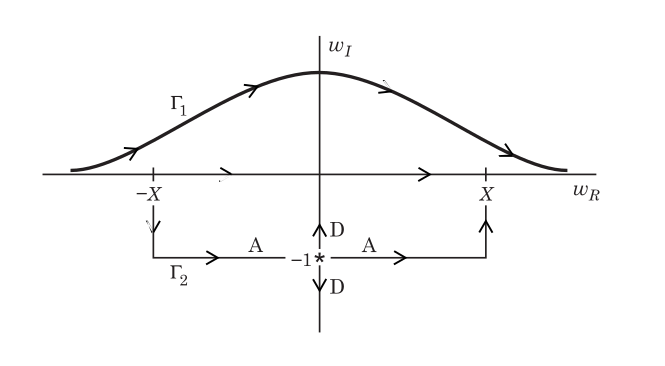
\includegraphics[width=12cm]{Contents/chapter5/figures/1.png}
      \caption{复$w$平面, $w =w_R + iw_I$, 表明由(\ref{玩具模型})和(\ref{有效哈密顿量})定义的玩具模型的积分路径. 最初的积分路径是沿着实轴, $w_I=0$. 柯西定理允许积分变形成任意轮廓$\Gamma_1$, 它在$w_R \rightarrow \pm \infty $处与实轴相连. 同样, 当$X \rightarrow +\infty$时, 分段轮廓$\Gamma_2$也可应用. 玩具模型在虚轴$w^*= -i$处有一个鞍点, 由星号标记. 通过鞍点的恒定相曲线具有$H_I=0$, 对应于线$w_I=-1$和$w_R=0$. 上升曲线标记$A$和下降曲线标记$D$}
      \label{复平面w}
\end{figure}
上升曲线是我们主要感兴趣的曲线, 因为它们可以通过轮廓$\Gamma_2$连接到原始的积分路径, 并对配分函数产生一个有限的结果. 当$ X \rightarrow +\infty$时在$w_R=\pm X$ 处轮廓片段的分布衰减为$\sim \exp(-pX^2/2)$,所以可以忽略. 这样, 我们就可以通过$w =x -i$, 将原来的积分正式地转化为恒定相路径$\Gamma$上的积分\\
\begin{equation}
\begin{aligned}
\mathcal{Z} &= \int_\Gamma \exp[-H(w)] \ dw = \int_\infty^\infty \exp[-H_R(x,-1)] \ dx\\
& =\int_\infty^\infty \exp[-p(1+x^2)/2] \ dx \label{恒定相路径积分}
\end{aligned}
\end{equation}
由于相因子$\exp(iH_I)$沿着积分路径不变, 所以最终积分不再具有振荡积分. 该积分可以用方程(B.1)得到精确结果$\mathcal{Z}=(2\pi/p)^{1/2}\exp(-p/2)$. 一个重要的观测结果是, 对于较大的$p$, 沿着恒定相路径上的积分由鞍点$x=0$时$H_R$的局部极小值決定. $p\rightarrow +\infty$時, 拉普拉斯型积分不能解析计算, 为其提供了渐近展开. \\

本文讨论的一维“玩具”模型有几个要点, 可以立即推广到像方程(\ref{配分函数})一样的高维的静态场理论中:\\

$\bullet$ 在定义的配分函数时, 场$w(\br)$的每个自由度的初始积分路径是沿实轴的. 尽管如此, 对于一个解析积分$\exp(-H[w])$, 它是有用的, 至少对多维复平面上的通过一个或多个鞍点$w^*(\br)$的恒定相“上升”轮廓(面)的积分路径有用. 相因子$\exp(iH_I[w])$沿这样的轮廓是恒定的, 从而消除了被积函数的振荡. \\

 $\bullet$通过对第四章模型的检验, 容易证明统计权重$\exp(-H[w])$和$\exp(-H_G[w])$是$w$的解析泛函. 因此, 上述变形对于所有模型都是可能的. 但是, 应该指出的是, 只有在巨正则系综中哈密顿量才解析, 且在正则系宗中, $H[w]$具有奇点,限制了解析区域. \\

$\bullet$鞍点场构型$w^*$对泛函积分在恒定相轮廓上变形有重要贡献, $w^*$代表平均场解. 在恒定相(上升)流形上, $H_R[w]$在鞍点上具有局部最小值. 鞍点场构型对积分的影响程度取决于一个“金兹伯格参数”的值, 类似于玩具模型中的$p$. 实际上, 很容易证明配位数$C=\rho_cR_g^3$是第四章中描述的许多模型的相关参数. 因此, $C\rightarrow +\infty$时, 这些模型的平均场近似变得精确. \\

$\bullet$在进行计算之前, 先确定复平面上鞍点的定性位置和方向是很有用的. 例如, 在模型$A$中, 要求$H[w^*]$或$H_G[w^*]$是实的意味着几乎所有鞍点$w^*(\br)$必须是纯虚的. 对于模型$B-E$, $w_{-}^*$和$w_{+}^{*}$分别是纯实的和纯虚的.利用虚轴上的松弛方案计算一个纯虚的鞍点是很方便的, 这是一个与物理积分路径正交的搜索方向. 对于这样的方案, 重要的是要认识到这很可能是$H_R[w]$的下降方向, 所以我们应该寻找一个局部最大值, 而不是一个局部最小值!\\
\subsection{多解}
对于大多数感兴趣的流体模型, 方程(\ref{H[w]相对w(r)的变化})有多个解, 对应于多个鞍点. 一个广义分类方案将这类鞍点识别为各向同性的, 即$w^*(\br)$独立于位置$\br$, 或各向异性的—$w(\br)$具有明显的位置相关性. 各向同性鞍点往往可以解析确定, 而各向异性鞍点通常需要数值方法进行计算. \\

一般来说, 人们可以将一个纯态鞍点与流体的每一个稳定或亚稳定相关联. 例如, $AB$型两嵌段聚合物的模型具有“纯态”鞍点, 可与无序相($D$), 层状相($L$), 柱状相($C$), 螺旋二十四面体($G$)和球形($S$)中间相关联. $L$, $C$, $G$和$S$鞍点是各向异性的且准周期的;稳定的S鞍点具有体心三次(bcc)对称. 对模型$E$其他纯态鞍点是已知的, 例如双金刚石($DD$)和超细粉体($HPL$)对称性的点已经被计算出来. 平均场理论中, 这些在整个$\mathcal{X}N$和$f$的参数空间都是亚稳态的. \\

各向异性的纯态点不一定是周期性的. 在这种情况下, 各向异性的结构通常是由适用于模型的边界条件决定的. 例如, 模型A在描述一个好溶剂中均聚合物的解时, 当在狄利克雷边界条件的约束几何中求解时, 它有一个唯一的、非均匀的纯态点$w^*(z)$. $\tilde{\rho}(z;[iw^*])$给出了平均场近似中与此势对应的段密度分布, 其中$\tilde{\rho}$是方程(4.75)的密度算子. 这类不均匀剖面的数值例子见图\ref{剖面}. 
\begin{figure}[H]
       \centering
        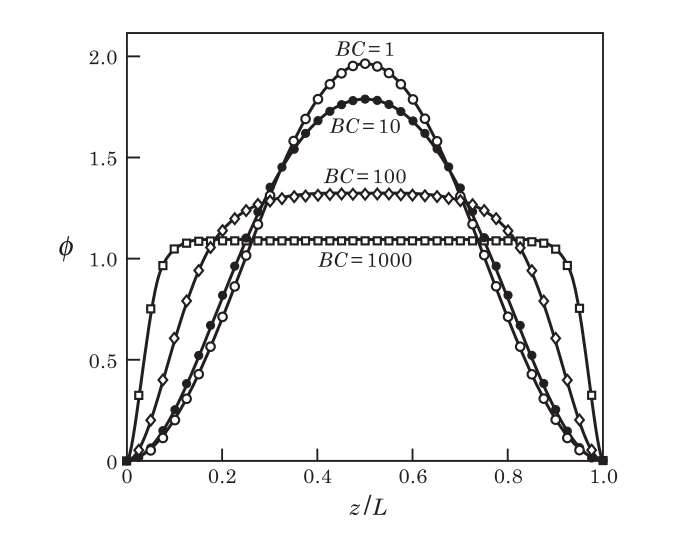
\includegraphics[width=12cm]{Contents/chapter5/figures/2.png}
       \caption{在一个简单的几何中求解模型$A$得到的平均场约密度剖面. 对于$BC=1$(开圆), $BC=10$(填充圆), $BC=100$(开菱形)和$BC=1000$(开方形)的数值结果. 固体线表示符合基于基态优势近似的解析表达式. 转载自Alexander-Katz等人. (2003年)}
        \label{剖面}
 \end{figure}

纯态鞍点是唯一的, 除了平移和旋转不改变能量$H[w^*]$. 即使在一类空间周期结构中, 对于一个特定的复杂流体模型, 也很难计算和评估所有纯态鞍点的稳定性. 在实际应用中, 我们主要感兴趣的是模型参数空间中具有一定稳定性区域对应的鞍点. 幸运的是, 最稳定的鞍点(即$H[w^*]$值最低的点)通常也是能量图形中吸引力最大的点, 因此可以通过大型单元模拟来识别它们, 使$w$场从随机初始构型中放松下来(参见章节5.3.4). 更普遍地, 对任意流体模型求方程(\ref{H[w]相对w(r)的变化})最小能量纯态解是全局优化中的一个不能解决的问题(Nocedal 和 Wright, 1999). \\

除了“纯态”点外, 还可以找到对应于缺陷态的方程(\ref{H[w]相对w(r)的变化})的各向异性的解. 它们之所以如此命名, 是因为它们反映了另一种完美的周期结构中的拓扑缺陷. 例如, 类似于二维六状晶体的位错, 两嵌段共聚物的柱状薄膜可能具有所谓的位错(Hammond等人, 2003年). 当圆柱体与薄膜的平面垂直排列时, 这样的面内位错会反映出相邻的柱状共聚物的“旋错对”, 一个是5个近邻, 另一个是7个. 如圖\ref{方格图}中所示, 除了这些旋错对外, 所有其他柱状都有6个最近的近邻. 由于纯态鞍点具有较低的能量, 与缺陷态对应的鞍点(如刚刚描述的位错)通常是亚稳的. 然而, 对于带有边界条件的方程(\ref{H[w]相对w(r)的变化})纯态解是不适应的, 如球体表面的晶化情况(Nelson, 1983), “缺陷状态”鞍点可以变得稳定. 也有理论和实验支持玻璃形成的系统拥有大量的(在系统尺寸下)的再结晶缺陷态(Monasson,1995年;Zhang和Wang, 2005). 冷却后, 这样的系统会被困在其中一种不稳定的状态中, 从而产生一种玻璃化转变. \\
\begin{figure}[H]
        \centering
         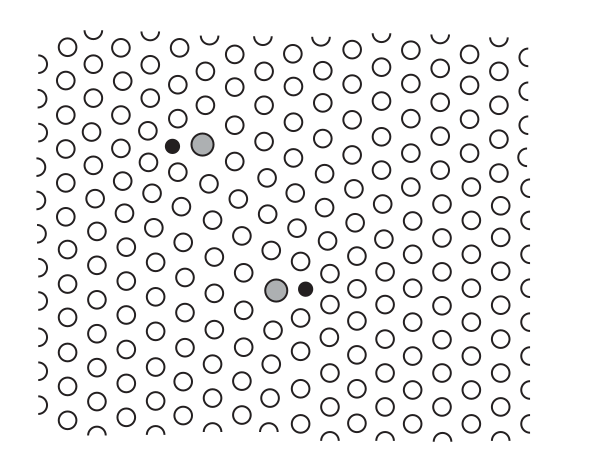
\includegraphics[width=12cm]{Contents/chapter5/figures/3.png}
    \caption{包含两个位错的柱状形成的块状聚合物的二维六状方格图. 每个位错本身就是一个由5个近邻(黑色)和7个近邻(灰色)的柱状构成的旋错对. 所有柱状都有6个近邻(白色). 与缺陷相关的应变能导致位错与位错之间的块状再分布. 实验和数值$SCFT$计算都知道这一点, 即在7倍旋错时产生一个$\sim 20\%$的大圆柱体, 在5倍旋错时产生一个$\sim 20\%$的小圆柱体(Hammond等人, 2003年). } 
           \label{方格图}
\end{figure}


第三种类型的鞍点是两个或多个纯态共存时产生的混合状态. 例如, 一个二元共混物的模型$C$和$D$表现出两种液相共存, 在足够大的片段相互作用参数$\mathcal{X}_{AB}$下, 两种相中都很富有. 因此, 方程(\ref{H[w]相对w(r)的变化})对这些模型的正则系宗版本具有混合状态解, 反映了两个均相的共存, 组成不同, 并由一个界面分开. 对于稳定的“混合态”鞍点解, 在种类保护和应用边界条件的约束下, 通过最小面积的考虑, 可以得到界面的几何构型. 类似于纯态解, 混合状态点可以与例如均匀平移或旋转的状态点相关联. 在分离纯态相的界面没有在理想拓扑排列中配置的情况下, 也可以找到亚稳的、缺陷的、混合态的鞍点解. \\


\section{均匀鞍点}
通常可以通过分析方法定位均匀的鞍点,例如,规范模型A场理论的方程(5.3)简化为
\begin{equation}
\frac{1}{u_0}w^*(r)+i\tilde{\rho}(\br;[iw^*])=0
\end{equation}
这里,在构造函数导数时应用了方程(4.75)中的密度算子$\tilde{\rho}(\br;[iw^*])$。在无界系统中,或在受周期性边界条件影响的立方体单元中,该方程的唯一解析解是均匀的,即$w^*(\br)=w^*$。从方程(3.25)和(3.22)得出$q(\br,s;[iw^*])=\exp(-iw^*s)$和$Q[iw^*]=\exp(-iw^*N)$以及方程(4.75)中$\tilde{\rho}(\br;[iw^*])=nN/V$,其与平均段密度$\rho_0$一致。因此,方程(5.11)简化为
\begin{equation}
w^*=-iu_0\rho_0
\end{equation}
由于排除了体积参数$u_0$和平均段密度$\rho_0$都是实数和正数的情况,因此势场的鞍点值$w^*$位于复数$w$平面的负虚轴上。这类似于第5.1.2节中讨论的玩具(toy)模型的情况。

在均匀鞍点处的规范模型A的有效哈密顿量由等式(4.72)估计为$H[w^*]=(1/2)u_0\rho_0^2V$。由此得出,聚合物溶液的Helmholtz自由能的平均场近似值由下面式子给出
\begin{equation}
A(n,V,T)=A_0+\frac{k_BT}{2}u_0\rho_0^2V
\end{equation}
这里$A_0=-k_BT\ln\calZ_0$是非相互作用聚合物的理想气体的自由能。在平均场近似中,自由能的过量部分仅由聚合物链段之间的平均相互作用能量产生,没有考虑它们的空间相关性。

对大规范模型A重复此分析是很有用的。鞍点方程相当于
\begin{equation}
\frac{\delta H_G[w]}{\delta w(\br)}\bigg|_{w=w^*}=\frac{1}{u_0}w^*(\br)+i\tilde{\rho}_G(\br;[iw^*])=0
\end{equation}
其中$\tilde{\rho}_G$是方程(4.76)中给出的分段密度算子。对于均匀$w^*(\br)=w^*$,可以发现
\begin{equation}
\tilde{\rho}_G(\br;[iw^*])=zN\exp(-iw^*N)=\frac{\left\langle n\right\rangle N}{V}\equiv\rho_0
\end{equation}
其中$\left\langle n\right\rangle=zVQ[iw^*]=zV\exp(-iw^*N)$是体积$V$中聚合物的平均数,而$\rho_0$是平均链段密度。由此可见,平均场满足以下超越方程
\begin{equation}
iw^*\exp(iw^*N)=u_0zN
\end{equation}
因为右端是实的和正的,所以该方程有唯一的解$w^*$,其位于任何聚合物活性$z$的负虚轴上。

与大规范模型A的热力学的关联通过以下公式将渗透压$\Pi$与$\calZ_G$联系起来
\begin{equation}
\begin{aligned}
\beta\Pi&=\frac{1}{V}\ln\calZ_G(z,V,T)\\
&\approx-\frac{1}{V}H_G[w^*]=\frac{\rho_0}{N}+\frac{1}{2}u_0\rho_0^2
\end{aligned}
\end{equation}
其中在上面公式的第二行中应用了平均场近似。因此,我们看到渗透压的平均场表达式包括与聚合物平均密度成比例的理想气体项的总和,$\rho_0/N$和与单位体积自由能中相应项的相互作用项组成。这些当然是众所周知的结果(de Gennes,1979)。对于第四章中介绍的其他模型的均匀平均场解,可以推导出类似的表达式。
\subsection{进一步近似}
更令人感兴趣的是鞍点方程(5.3)的非均匀解。通常需要数值分析的方法来得到这种平均场解的精确描述。数值方法的讨论推迟到第5.3节;在这里,我们考虑进一步的分析近似,使不均匀的鞍点方程易于处理。这些近似基于第3.4节中提出的方案,用于估计外部势场中单链的统计特性。
\subsection{弱不均匀性-RPA}
可以与平均场近似一起应用的一种重要的近似类型是弱不均匀性扩展。在方程(5.3)的解几乎是一致的情况下,我们可以用方程(3.113)类比得出
\begin{equation}
w^*(\br)=w_0+\omega^*(\br)
\end{equation}
其中$w_0\equiv(1/V)\int w^*(\br)\mathrm{d}\br$是体积平均的平均场势场,假设偏差$\omega^*(\br)$与$w_0$相比在任何地方都很小,可以遵循3.4.1节的流程来产生弱的不均匀性扩展。这种扩展在聚合物文献中通常称为随机相近似,或RPA(de Gennes,1969;de Gennes,1979)。我们用规范模型A来说明它。

规范模型A的鞍点方程在方程(5.11)中给出。代替方程(5.18)并应用方程(3.134)和(4.75)导出以下扩展:
\begin{equation}
u_0^{-1}\omega^*(\br)+\rho_0N\int g_D(\left|\br-\br'\right|)\omega^*(\br')\mathrm{d}\br'+O((\omega^*)^2)=0
\end{equation}
其中方程(5.12)用于取消主导齐次项,$g_D$是方程(3.133)的Debye函数。方程(5.19)的唯一解是$\omega^*(\br)=0$,这与我们之前的声明一致,即规范模型A的整体或具有周期性边界条件的单元的唯一鞍点是均匀解$w^*(\br)=w_0$。

RPA扩展还可用来观察密度函数$F[\rho]$的形式,这是第4.10节DFT形式的核心,在平均场近似中,规范模型A的方程(4.207)简化为
\begin{equation}
\rho(\br)\approx\tilde{\rho}(\br;[iw^*+J])
\end{equation}
我们用$\rho(\br)$的简写代替$\left\langle\hat{\rho}(\br)\right\rangle_J$。该等式确定由任意外部势场$J(\br)$产生的平均段密度$\rho(\br)$。此外,在平均场近似中,方程(4.205)的配分函数简化为$\calZ_C[J]\approx\calZ_0\exp(-H[w^*,J])$,在这两个表达式中,鞍点$w^*(\br)$由下式确定
\begin{equation}
\frac{\delta H[w,J]}{\delta w(\br)}\bigg|_{w=w^*}=u_0^{-1}w^*(\br)+i\tilde{\rho}(\br;[iw^*+J])=0
\end{equation}
通过选择$J$,使其幅值较弱并且具有较好的体积平均值,即$(1/V)\int J(\br)\mathrm{d}\br=0$,方程(5.21)的右端可以类似于方程(5.19)的RPA扩展得出。在$J$的领先秩序,
\begin{equation}
\begin{aligned}
\int[u_0^{-1}\delta(\br-\br')&+\rho_0Ng_D(\left|\br-\br'\right|)]\omega^*(\br')\mathrm{d}\br'\\
&=i\rho_0N\int g_D(\left|\br-\br'\right|)J(\br')+O(J^2)
\end{aligned}
\end{equation}
该结果的傅里叶变换产生一下关于$\omega^*$和$J$的公式:
\begin{equation}
\hat{\omega}^*(\bk)=\frac{iu_0\rho_0N\hat{g}_D(x)}{1+u_0\rho_0N\hat{g}_D(x)}\hat{J}(\bk)+O(J^2)
\end{equation}
其中$x=k^2R_g^2$是无量纲的平方波数,其具有未受扰动的回旋半径的平方,$R_g^2=Nb^2/6$。

下一步是使用方程(5.23)和(3.131)扩展方程(4.206)中给出的函数$H[w^*,J]$。这将得出:
\begin{equation}
H[w^*,J]=H_0-\frac{1}{2V}\sum\limits_{\bk}\frac{\rho_0N\hat{g}_D(x)}{1+u_0\rho_0N\hat{g}_D(x)}\hat{J}(\bk)\hat{J}(-\bk)+O(J^3)
\end{equation}
其中$H_0\equiv(1/2u_0)Vw_0^2+w_0Nn$是对哈密顿量的均匀贡献。构造自由能函数$F[\rho]$所需的最后一步是通过方程(4.199)利用勒让德变换将$J$变为$\rho$,即
\begin{equation}
F[\rho]=-\ln\calZ_0+H[w^*,J]-\int J(\br)\rho(\br)\mathrm{d}\br
\end{equation}
这个变换需要扩展方程(5.20)来建立$J$和$\rho$之间的关系。应用方程(3.134)得
\begin{equation}
\widehat{\Delta\rho}(\bk)=-\frac{\rho_0N\hat{g}_D(x)}{1+u_0\rho_0N\hat{g}_D(x)}\hat{J}(\bk)+O(J^2)
\end{equation}
其中$\Delta\rho(\br)\equiv\rho(\br)-\rho_0$是单体密度场的不均匀部分。结合方程(5.24)-(5.26)得到所需的自由能泛函
\begin{equation}
F[\rho]=F_0+\frac{1}{2V}\sum\limits_{\bk}\left(\frac{1}{\rho_0N\hat{g}_D(x)}+u_0\right)\widehat{\Delta\rho}(\bk)\widehat{\Delta\rho}(-\bk)+O(\Delta\rho^3)
\end{equation}
其中$F_0$是均匀流体的平均场自由能。

方程(5.27)是对应于模型A的弱非均匀聚合物溶液的自由能(以$k_BT$为单位)的表达式。在适用平均场近似且密度不均匀性小的程度上是有效的。正如将在第6章讨论的那样,平均场近似适用于模型A,其浓度足够高满足
\begin{equation}
C\gg B\equiv\frac{u_0N^2}{R_g^3}
\end{equation}
其中$C=nR_g^3/V$是在方程(5.5)中引入的无量纲链浓度,$B$是无量纲消除体积参数。

方程(5.27)的一个有用的应用是估计聚合物溶液的均相相对于小幅度密度扰动的稳定性。通过检查二次系数可以确定稳定性。
\begin{equation}
\hat{\Gamma}_2(k)=\frac{1}{\rho_0N\hat{g}_D(k^2R_g^2)}+u_0
\end{equation}
作为波数$k=\left|\bk\right|$的函数。由于$\hat{g}_D(x)$是$x$的单调递减函数,因此,$\hat{\Gamma}_2(k)$的最小值与$k=0$一致。均匀相或螺旋线的稳定极限因此对应于
\begin{equation}
\hat{\Gamma}_2(0)=\frac{1}{\rho_0N}+u_0=0
\end{equation}


















































































    \section{基态优势$Ground state dominance$}
%\label{sec.example}
    3.4.3节中的基态优势近似是一种可以和平均场近似结合使用的非常有效的方法.
    当高分子聚合物限制在与$R_{g}$的尺度相比较小的区域上时,
    这种组合是比较合适的.
    我们通过回到现在所熟悉的正则系综中模型$A$的自由能问题泛函的推导来引入这个主题.
    \par
    正则模型$A$中的平均场公式(5.20)和(5.21)可以简便地重新表示成
    \label{subsec.equations}
    \begin{equation}
        \begin{aligned}
        \rho(r)=\hat{\rho}(\bm{r};[i\omega^{*}+J]),
            i\omega^{*}(\bm{r})=u_{0}\rho(\bm{r}). 
                   \end{aligned}
        \label{eq5.51}
    \end{equation}
    公式(3.167)和(4.75)可以进一步和基态优势近似结合将会得到
    \label{subsec.equations}
    \begin{equation}
        \begin{aligned}
            \rho(\bm{r})=\hat{\rho}(\bm{r};[i\omega^{*}+J])=nN[\psi(\bm{r})]^{2}.
                   \end{aligned}
        \label{eq5.52}
    \end{equation}
    公式中的基态特征函数$\psi(\bm{r})$满足公式(3.160)且$\omega\longrightarrow
    i\omega^{*}+J$, 即
    \label{subsec.equations}
    \begin{equation}
        \begin{aligned}
            \frac{b^2}{6}\nabla^{2}\psi(\bm{r})=[i\omega^{*}(\bm{r})+J(\bm{r})-\Lambda]\psi(\bm{r}).
                   \end{aligned}
        \label{eq5.53}
    \end{equation}
其中$\Lambda$是基态特征函数. 由外场$J$可以表示成
    \label{subsec.equations}
    \begin{equation}
        \begin{aligned}
            J[\rho]=\frac{b^{2}}{6\psi(\bm{r})}\nabla^{2}\psi(\bm{r})-u_{0}\rho+\Lambda.
                   \end{aligned}
        \label{eq5.54}
    \end{equation}
将这个结果代入公式(4.206)和(5.25)得到下面的密度泛函:
    \label{subsec.equations}
    \begin{equation}
        \begin{aligned}
            F[\rho]=\int d\bm{r}\
            \left(-\frac{nNb^{2}}{6}\psi\nabla^{2}\psi+\frac{u_{0}}{2}\rho^{2}-\Lambda\rho
            \right).
                   \end{aligned}
        \label{eq5.55}
    \end{equation}
其中项$-n\ln\ Q[i\omega^{*}+J]$被忽略了, 因为它比所示项的$O(1/N)$还要小.
\par
接下来的任务就是将公式(\ref{eq5.55})中包含$\psi$的项重新表示成$\rho$的泛函.
(\ref{eq5.52})微分产生$|\nabla\psi|^{2}=|\nabla\rho|^{2}/(4nN\rho)$,
将其代入(\ref{eq5.55})并分部积分会推出自由能泛函
    \label{subsec.equations}
    \begin{equation}
        \begin{aligned}
            F[\rho]=\int d\bm{r}\
            \left(\frac{b^{2}}{24\rho}|\nabla\rho|^{2}+\frac{u_{0}}{2}\rho^{2}-\Lambda\rho
            \right).
                   \end{aligned}
        \label{eq5.56}
    \end{equation}
在最后的这个表达式中, 保留了与$\Lambda$成比例的项.
或者$\Lambda$也可以被吸收在拉格朗日乘子(化学势)$\mu$中,
其在(4.202)中可以用来构造巨势$\Omega[\rho]$和加强限制$\int d\bm{r}=nN$.
\par
(\ref{eq5.56})给出的基态自由能泛函比(3.169)给出的泛函$F_{2}[\rho]$惊人地小.
事实上, 在$F_{2}[\rho]$代入$\omega\longrightarrow
i\omega^{*}/2=u_{0}\rho/2$会马上推出(\ref{eq5.56}).
从公式我们可以看到非均匀聚合物溶液的自由能泛函在基态可以近似作为$Lipshitz$熵项和平均场段与段之间反应项的和.
$Lipshitz$熵反应了与非均匀密度分布$\rho(\bm{r})$相关的构象熵惩罚.
\par
公式(\ref{eq5.56})和由慢梯度推导的自由能泛函(5.49)在形式上很相似.
在基态表达式中平移熵项$(\rho/N)\ln\rho$消失了, 当$N\longrightarrow \infty$,
或者$\xi/R_{g}\longrightarrow 0$是合理的,
其中$\xi$是聚合物位置所在区域的宽度. 
另外$Lifshitz$熵项的平方梯度系数在公式(5.49)中是$1/36$,
在公式$(\ref{eq5.56})$中是$1/24$. 这种矛盾的起源可以追溯到这样一个事实,
在尺度$R_{g}$上, $1/36$适用于缓慢密度变化, 而$1/24$则适用于快速密度变化.
事实上, 我们可以看到对于小振幅密度不均匀性,
慢梯度展开(5.49)中的系数$1/36$和$RPA$近似(5.27)对于$kR_{g}\ll 1$是保持一致的.
在快速密度变化的相反的极限, 即$kR_{g}\gg 1$,
在公式(\ref{eq5.56})$RPA$展开产生系数$1/24$. 换言之,
$RPA$和基态优势近似在小振幅上和在$R_{g}$尺度变换上大时是保持一致的.
然而基态表达式(\ref{eq5.56})并不局限于弱非均匀性.
\par
基态优势近似的第二个应用, 我们将考虑最初由$Helfand$和$Tagami$($Helfand\ and\ Tagami, 1971$)解决的对称聚合物与聚合物界面的经典问题.
他们研究了一类不可压共聚物混合模型的解析解,
这种模型是具有等统计段长度和聚合度的模型$C$的一种特殊的情况,
即$b_{A}=b_{B}=b$且$N_{A}=N_{B}=N$. 这个解依赖于平均场和基态优势近似.
其满足如果$\chi_{AB}\ll 1$, $N\gg 1$, 则$\chi_{AB}N\gg 1$. 强分离极限是指:
体系由两个在聚合物$A$和$B$中几乎纯的共存相组成, 通过一个窄的界面分开,
其宽度$\xi$比旋转半径$R_{g}=b(N/6)^{1/2}$要小的多.
\par
$Helfand$和$Tagami$考虑的情况对应于一个平面界面, 位于$z=0$处,
将在$z\longrightarrow +\infty$的$A$共聚物的纯相和在$z\longrightarrow
-\infty$的$B$共聚物的纯相分开. 平均场方程对应于
\label{subsec.equations}
    \begin{equation}
        \begin{aligned}
            \frac{\delta H[\omega_{\pm}]}{\delta
            \omega_{+}(z)}|_{\omega_{\pm}=\omega^{*}_{\pm}}=i\rho_{0}[\phi_{A}(z;
            [\omega^{*}_{A}])+\phi_{A}(z;
            [\omega^{*}_{A}])-1]=0.
                   \end{aligned}
        \label{eq5.57}
    \end{equation}
\label{subsec.equations}
    \begin{equation}
        \begin{aligned}
            \frac{\delta H[\omega_{\pm}]}{\delta
            \omega_{-}(z)}|_{\omega_{\pm}=\omega^{*}_{\pm}}=\rho_{0}[(2/\chi_{AB})\omega^{*}_{-}(z)-\phi_{A}(z;
            [\omega^{*}_{A}])+\phi_{A}(z;
            [\omega^{*}_{A}])]=0.
                   \end{aligned}
        \label{eq5.58}
    \end{equation}
其中$\omega_{A}=i\omega_{+}-\omega_{-}$,
$\omega_{B}=i\omega_{+}+\omega_{-}$是$A,B$单体的共轭化学势,
且$\phi_{K}$是$K$类单体的局部体积分数($K=A$或$B$), 由
\label{subsec.equations}
    \begin{equation}
        \begin{aligned}
        \phi_{K}(\bm{r}; [\omega_{K}])\equiv \hat{\rho}_{K}(\bm{r};
            [\omega_{K}])\rho_{0}.
        \end{aligned}
        \label{eq5.59}
    \end{equation}
这第一个平均场方程(\ref{eq5.57})表示了不可压缩条件,
即两种物质在每个位置的的体积分数之和必须为1. 第二个鞍点方程(\ref{eq5.58})表示,
交换化学势场和$A$类的体积分数有关,
在自洽场近似中$\omega^{*}_{-}(z)=\chi_{AB}[\phi_{A}(z; [\omega^{*}_{A}]-1/2)]$.
\par
方程(\ref{eq5.57})和(\ref{eq5.58})是一个难以处理的方程,
因其在鞍点$\omega^{*}_{\pm}(z)$处依赖与体积分数$\phi_{K}(z; [\omega^{*}_{K}])$.
然而, 利用基态优势近似, 体积分数可以简化成.
\label{subsec.equations}
    \begin{equation}
        \begin{aligned}
            \phi_{K}(z; [\omega^{*}_{K}])\approx[\psi_{K}(z)]^2.
        \end{aligned}
        \label{eq5.60}
    \end{equation}
其中基态特征函数$\psi_{K}(z)$满足
\label{subsec.equations}
    \begin{equation}
        \begin{aligned}
        \frac{b^{2}}{6}\frac{d^{2}}{dz^{2}}\psi_{A}(z)=[i\omega^{*}_{+}(z)-\omega^{*}_{-}(z)-\Lambda_{A}]\psi_{A}(z).
        \end{aligned}
        \label{eq5.61}
    \end{equation}
\label{subsec.equations}
    \begin{equation}
        \begin{aligned}
        \frac{b^{2}}{6}\frac{d^{2}}{dz^{2}}\psi_{B}(z)=[i\omega^{*}_{+}(z)+\omega^{*}_{-}(z)-\Lambda_{B}]\psi_{B}(z).
        \end{aligned}
        \label{eq5.62}
    \end{equation}
在这些方程中出现的基态特征值$\Lambda_{K}$的选择如下所述.
我们采用了与公式(3.161)不同的标准特征函数; 即$\int\
d\bm{r}\psi^{2}_{K}=V\phi_{K_{0}}$,
其中$\phi_{K_{0}}$是包含在体系中$K$类聚合物段的平均体积分数.
\par
在适当的边界条件下, 在两个共聚相之间可以形成一个单平面界面. 特别地,
当共存相是纯的时候, 正如渐进情况$\chi_{AB}N\longrightarrow \infty$,
有$\psi_{A}(+\infty)=\psi_{B}(-\infty)=1$,
$\psi_{A}(-\infty)=\psi_{B}(+\infty)=0$. 下面的梯度条件也适用于$K=A, B$:
$\psi^{'}_{K}(\pm\infty)=\psi^{"}_{K}(\pm\infty)=0$.
因为方程(\ref{eq5.61})和(\ref{eq5.62})是和边界条件是保持一致的,
必须满足$\Lambda_{A}=\Lambda_{B}=\Lambda$,
$i\omega_{+}(\pm\infty)-\chi_{AB}/2-\Lambda=0$.
可以选择一个简单的但任意的压力场$\omega_{+}(\pm\infty)=0$,
其暗示了$\lambda=-\chi_{AB}/2$. 因此方程(\ref{eq5.61})和(\ref{eq5.62})简化成
\label{subsec.equations}
    \begin{equation}
        \begin{aligned}
            \frac{b^{2}}{6}\frac{d^{2}}{dz^{2}}\psi_{A}(z)=[i\omega^{*}_{+}(z)+\chi_{AB}\phi_{B}(z)]\psi_{A}(z).
        \end{aligned}
        \label{eq5.63}
    \end{equation}
\label{subsec.equations}
    \begin{equation}
        \begin{aligned}
            \frac{b^{2}}{6}\frac{d^{2}}{dz^{2}}\psi_{B}(z)=[i\omega^{*}_{+}(z)+\chi_{AB}\phi_{A}(z)]\psi_{B}(z).
        \end{aligned}
        \label{eq5.64}
    \end{equation}
因此$A$聚合物段受到的平均势场是压力项$i\omega^{*}_{+}(z)$和$B$段局部接触反应项$\chi_{AB}\phi_{B}(z)$之和.
同样地$B$聚合物也受到相同的压力场, 但是反应势$\chi_{AB}\phi_{A}(z)$与$A$段的局部体积分数成比例
\par
$Helfand$和$Tagami$证明了当$K=A, B$时, 由\ref{eq5.57}),
(\ref{eq5.60})组成的五个方程对上述平面边界条件具有解析解, 这个解对应于
\label{subsec.equations}
    \begin{equation}
        \begin{aligned}
            \phi_{A}(z)=1-\phi_{B}(z)=\frac{1}{1+\exp{-z\xi}}.
        \end{aligned}
        \label{eq5.65}
    \end{equation}
\label{subsec.equations}
    \begin{equation}
        \begin{aligned}
            \psi_{K}(z)=[\phi_{K}(z)]^{1/2}.
        \end{aligned}
        \label{eq5.66}
    \end{equation}
\label{subsec.equations}
    \begin{equation}
        \begin{aligned}
            i\omega^{*}_{+}(z)=-3\chi_{AB}\phi_{A}(z)\phi_{B}(z).
        \end{aligned}
        \label{eq5.67}
    \end{equation}
其中$\xi$是界面宽度大小, 定义为
\label{subsec.equations}
    \begin{equation}
        \begin{aligned}
            \xi=\frac{b}{2(6\chi_{AB})^{1/2}}.
        \end{aligned}
        \label{eq5.68}
    \end{equation}
%\subsection{图像}
\label{subsec.figure}
\begin{figure}[htbp]
    \centering
%    \begin{minipage}[t]{0.2\linewidth}
    \centerline{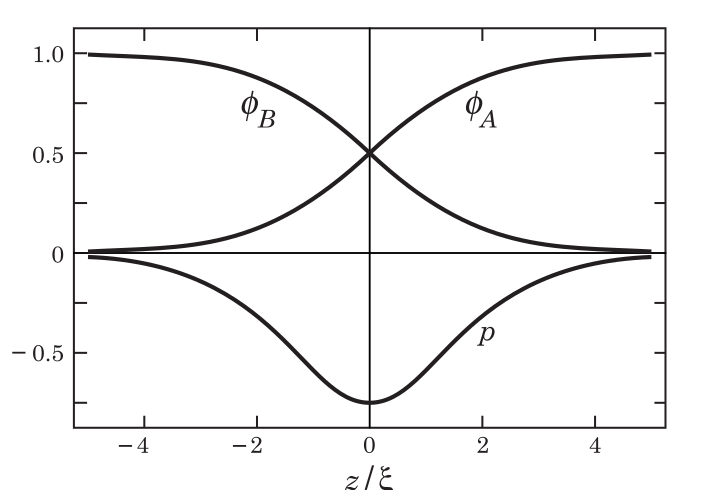
\includegraphics[scale=0.4]{./Contents/chapter5/figures/fig4.png}}
 %       \footnotesize{\centerline{(a)}}
 %   \end{minipage}
%    \hspace{0.2\linewidth}
%    \begin{minipage}[t]{0.2\linewidth}
%%        \centerline{\includegraphics[scale=0.4]{figure/figure2.png}}
%        \footnotesize{\centerline{(b)}}
%    \end{minipage}
    \caption{(书中的图5.4)\
    对称聚合物-聚合物界面的界面曲线的$Helfand-Tagami$解. $A,
    B$聚合物段的体积分数分别标记了$\phi_{A}$和$\phi_{B}$.
    整段的体积分数是单位1. $p$曲线表示压力场$p(z)\equiv
    i\omega^{*}_{+}(z)/\chi_{AB}$.}
	\label{fig.1}
\end{figure}




\par
与$Helfand-Tagami$解有关的平衡体积分数曲线$\phi_{A}(z)$和$\phi_{B}(z)$如图()所示.
界面宽度$\xi$与$A, B$所在区域宽度有关.
混合是与由$\chi_{AB}$参数化的$A-B$接触能相反的, 与扩散界面提供的构象熵成正比的.
压力场$i\omega^{*}_{+}(z)$是负的且位于界面区域. 场的作用将聚合物吸引到界面上,
从而在所有位置看来都是均匀的段密度.
\par
在章节$3.4.3$基态优势近似的有效性依赖于局部化学势域, 其远远小于$R_{g}$,
在本例中局部势就是压力场$i\omega^{*}_{+}(z)$,
不是约束整条链而是形成界面链段的环. 压力场的范围和界面宽度$\xi$是同阶的,
这个范围满足规则$\xi/R_{g}=1/[2(\chi_{AB}N)^{1/2}]\ll 1$, $\chi_{AB}N\gg 1$.
同样地, 平均场近似的有效性要求$C\gg 1$, 其中$C$是公式(5.5)定义的配位数.
因为在熔融状态下$C\sim \rho_{0}b^{3}N^{1/2}$, 只要$A$和$B$都是高分子量的,
这个条件就满足了, 即$N\gg 1$. 最后, 为使$Helfand-Tagami$解是有效的,
界面宽度$\xi$必须不能低于介观尺度. 换言之, 必须有$\xi\gg
b$,或等价地$\chi_{AB}\ll 1$. 只要满足条件$\chi_{AB}\ll 1$和$\chi_{AB}N\gg
1$,我们就认为$Helfand-Tagami$解是准确的. 
\par
非常重要的是我们要注意到公式(\ref{eq5.68})描述的的是固有的界面宽度,
在流体-流体界面实验中测量了界面宽度, 它包含了界面的长波长表面波动张力,
因此超出了固有界面宽度(Weeks,\ 1977;\ Huse\ et\ al.,\ 1985;\ Binder\ et\ al.,\
2001). 这样的表面波动张力可以被看作是一种特殊的场波动, 尤其是对与层几何.
\par
对称聚合物-聚合物界面的表面张力可以由$Helfand-Tagami$解获得,
注意到张力是每单位表面面积多余的自由能(Chandler,\ 1987), 且在平均场近似中,
$A(n_{A},\ n_{B},\ V,\ T)\approx k_{B}T\ H[\omega^{*}_{+},\ \omega^{*}_{-}]$.
通过公式(4.98), 界面张力可以由

\label{subsec.equations}
    \begin{equation}
        \begin{aligned}
            \gamma&=k_{B}T\rho_{0}\int^{+\infty}_{-\infty}\ dz\left(
            \frac{1}{\chi_{AB}}[\omega^{*}_{-}(z)]^{2}-i\omega^{*}_{+}(z)-\frac{1}{4}\chi_{AB}\right),
            \\
            &=-k_{B}T\rho_{0}\int^{+\infty}_{-\infty}\ dz\ (
            \chi_{AB}\phi_{A}(z)\phi_{B}(z)+i\omega^{*}_{+}(z)),
            \\
            &=2k_{B}T\rho_{0}\chi_{AB}\int^{+\infty}_{-\infty}\ dz\
            \phi_{A}(z)\phi_{B}(z),
            \\
            &=k_{B}T\rho_{0}(\chi_{AB}/6)^{1/2}.
        \end{aligned}
        \label{eq5.69}
    \end{equation}
因此强分离聚合物-聚合物界面的表面张力是与聚合物分子量无关的,
它的尺度是$Flory$相互作用参数$\chi_{AB}$的平方根.
\par
一个简单的缩放参数可以用来更好的理解公式(\ref{eq5.68})和(\ref{eq5.69}).
正如图(5.5)所示, 界面区域可以看作是相互混合的环的区域的宽度.
界面宽度$\xi$可以表示环路相互混合的区域的宽度.
考虑一个典型的包含$g$统计段的环, $g$的值可以看作是均分估计, 即:
一个环表示一条链对不同聚合物相的相互渗透,
这种渗透只能在成本为$O(k_{B}T)$的情况下才能发生.
带有$g$个段的环的能量损耗是$\sim g\chi_{AB}k_{B}T$, 因此我们可以得出结论$g\sim
1/\chi_{AB}$. 当$\chi_{AB}\ll 1$时, 这是一个很大的数.
因为的每个环的强作用力只与热能尺度有关系,
界面宽度可以估计成一个未受干扰的$g$段聚合物的大小, 即: $\xi\sim bg^{1/2}\sim
b/\chi_{AB}^{1/2}$. 这个尺度很显然是与公式(\ref{eq5.68})是保持一致的. 最后,
界面张力可以估计成由$A-B$接触引起的界面多余自由能密度($\sim
k_{B}T\rho_{0}\chi_{AB}$)乘以区域宽度$\xi$,即得到公式$\gamma\sim
k_{B}T\rho_{0}b\chi_{AB}^{1/2}$.
这个结果很显然是与公式(\ref{eq5.69})是保持一致的.

\label{subsec.figure}
\begin{figure}[htbp]
    \centering
%    \begin{minipage}[t]{0.2\linewidth}
    \centerline{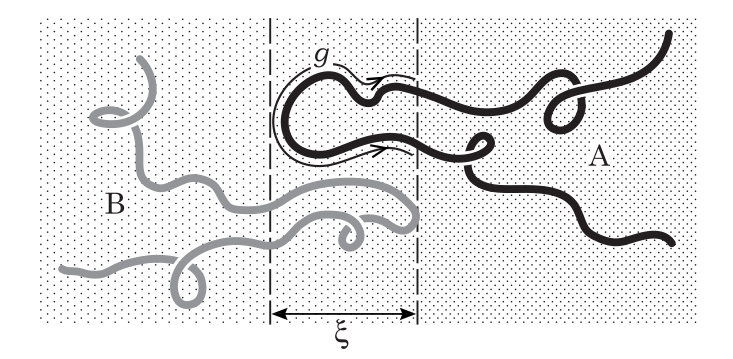
\includegraphics[scale=0.4]{./Contents/chapter5/figures/fig5.png}}
 %       \footnotesize{\centerline{(a)}}
 %   \end{minipage}
%    \hspace{0.2\linewidth}
%    \begin{minipage}[t]{0.2\linewidth}
%%        \centerline{\includegraphics[scale=0.4]{figure/figure2.png}}
%        \footnotesize{\centerline{(b)}}
%    \end{minipage}
    \caption{(书中的图5.5)\ 聚合物-聚合物界面的链构象示意图.
    一条穿过界面的聚合物链贡献了带有$g$段的环.
    且$A$环和$B$环混合穿过宽度为$\xi$的区域.}
	\label{fig.2}
\end{figure}



\subsubsection{强拉伸}
里另外一个有效的技术就是(3.4.4.2)节中描述的"强拉伸"近似与平均场近似的组合.阐释这种方法的一个有用的背景就是用模型$K$描述的溶液聚合物刷.
在足够高的密度系链下,刷中的聚合物被强烈拉伸, 可以采用这种经典的近似.
\par
在平均场近似中, (实数)势$\mu(z)\equiv
i\omega^{*}(z)$和平均段密度$\rho_{z}\equiv \hat{\rho}(z;
[i\omega^{*}])$在刷中每一个位置处成立关系
\label{subsec.equations}
    \begin{equation}
        \begin{aligned}
          \mu(z)=u_{0}\rho(z).
        \end{aligned}
        \label{eq5.70}
    \end{equation}
其中采用的是图(4.7)中的坐标体系. 经典的路径$z(s)$开始与嫁接面$z(0)=0$,
终止与$z(N)=z_{0}$, 满足公式(3.194), 即
\label{subsec.equations}
    \begin{equation}
        \begin{aligned}
            \frac{3}{b^{2}}\frac{d^{2}}{ds^{2}}z(s)=\frac{d\mu(z(s))}{dz(s)}.
        \end{aligned}
        \label{eq5.71}
    \end{equation}
其中尺寸单位已经恢复了. 因为不管末端位置是什么, 刷中所有的链都具有$N$个统计段,
"等时间限制"说明$\mu(z)$经典的近似必须是调和势, 即$\mu(z)=C_{1}-C_{2}z^{2}$.
带有这样的调和势, 并带有条件$z(0)=0$, $z(N)=z_{0}$,
且$[dz(s)/ds]_{s=N}=0$(在自由链端没有张力), 方程(\ref{eq5.71})可以求解出来.
经典路径
\label{subsec.equations}
    \begin{equation}
        \begin{aligned}
            z(s)=z_{0}\sin(\pi s/(2N)).
        \end{aligned}
        \label{eq5.72}
    \end{equation}
平方项系数
\label{subsec.equations}
    \begin{equation}
        \begin{aligned}
            C_{2}=\frac{3\pi^{2}}{8b^{2}N^{2}}.
        \end{aligned}
        \label{eq5.73}
    \end{equation}
第二个系数$C_{1}$可以通过保持分段关系
\label{subsec.equations}
    \begin{equation}
        \begin{aligned}
            \sigma N=\int^{h}_{0}dz\ \rho(z)=u_{0}^{-1}\int^{h}_{0}dz\
            (C_{1}-C_{2}z^{2}).
        \end{aligned}
        \label{eq5.74}
    \end{equation}
其中$h=(C_{1}/C_{2})^{1/2}$是聚合物刷厚度, 定义$\rho(h)=0$.
公式(\ref{eq5.74})的相当于是
\label{subsec.equations}
    \begin{equation}
        \begin{aligned}
            C_{1}=\frac{\sigma u_{0}N}{h}+\frac{C_{2}h^{2}}{3}.
        \end{aligned}
        \label{eq5.75}
    \end{equation}
通过组合这些结果, 我们得到了一个关于平衡刷厚度的重要公式(Milner\ et\ al., 1988)
\label{subsec.equations}
    \begin{equation}
        \begin{aligned}
            h=(\frac{4}{\pi^{2}})^{1/3}(\sigma u_{0})^{1/3}b^{2/3}N.
        \end{aligned}
        \label{eq5.76}
    \end{equation}
这公式有效的一个标准是聚合物被拉伸到一个高度,
其远远超过了它们未受干扰的尺度,$h/R_{g}\gg 1$. 相当于$(\sigma
u_{0}/b)^{1/3}N^{1/2}\gg 1$, 或者等价于$(\sigma R^{2}_{g})B\gg 1$,
其中$B$是由(5.28)定义的无量纲体积分数参数.
我们将可以看到参数$B$将在第六章中, 在聚合物溶液中评估排除体积效应的强度起到一个重要的作用. 
\par
在平均场密度近似和强拉伸近似的组合中,
平衡段密度曲线$(u_{0}/C_{1})\rho(z)=1-(z/h)^{2}$在图(5.6)中画出来了.
这个抛物曲线反应了在高嫁接密度时平均场段密度分布(Milner, 1990). 然而,
图中的虚线显示, 强拉伸近似对平均场曲线的近似并不是一致有效的,
在表面和刷的外边界周围都是由偏差的.
在$z=0$附近的耗长边界层已经在(4.9.4)讨论过了. 事实上,
带有适用于在$z=0$的传播子的$Dirichlet$条件的模型$K$的全平均场的解显示了一个尖锐层,
正如图(5.6)的虚线所示. 密度梯度随着嫁接的密度的增大而增大.
从图我们可与清晰地看到, 强拉伸近似只适用于边界层外, 其中$\mu(z)$缓慢变化,
且在$z=0$处符合黎曼边界条件. 同样地, 在刷的外边界,
平均场方程的近似解表现了密度曲线的缓慢变化(Milner, 1990),
与突然终止与$z=h$的抛物曲线相反. 外边界层是由于在刷子边缘的强烈拉伸引起的,
这个区域h中, 平均密度曲线是多个聚合物构象的结果.
$Matsen$最近对于"干聚合物刷"的强拉伸近似和平均场近似之间,
以及在干刷和化学性质相同的均聚物熔体之间的界面做了相似的比较(Matsen, 2004;
Matsen, 2005a).


\label{subsec.figure}
\begin{figure}[htbp]
    \centering
%    \begin{minipage}[t]{0.2\linewidth}
    \centerline{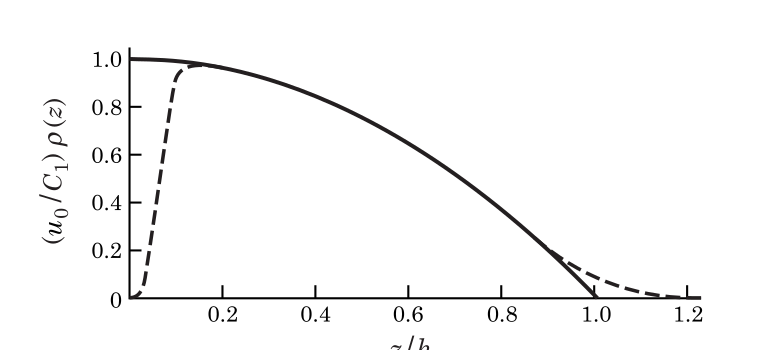
\includegraphics[scale=0.4]{./Contents/chapter5/figures/fig6.png}}
 %       \footnotesize{\centerline{(a)}}
 %   \end{minipage}
%    \hspace{0.2\linewidth}
%    \begin{minipage}[t]{0.2\linewidth}
%%        \centerline{\includegraphics[scale=0.4]{figure/figure2.png}}
%        \footnotesize{\centerline{(b)}}
%    \end{minipage}
    \caption{(书中的图5.6)\
    聚合物刷的模型$K$的平均场近似和强拉伸近似组合得到的段密度曲线$\rho(z)$的示意图.
    在高嫁接密度下, 实曲线表示全平均场密度分布, 边界层如虚线所示. 在表面附近,
    经典近似采用黎曼边界条件且忽略了狭窄的耗尽层. 在刷的外边界,
    强拉伸近似衰弱下来形成了一条光滑额曲线.}
	\label{fig.3}
\end{figure}



\par
模型$K$的强拉伸理论和全平均场解都忽略了场波动. 在嫁接点$\sim\sigma^{1/2}$, 当短波长低于平均间距的情况下,
场波动是最强烈的, 且引起了刷的不能在平均场近似中看到的一个局部的排除体积效应.
排除体积效应可以通过利用"斑点事件"近似地纳入平均场理论中(Milner\ et\ al, 1988;
Netz\ and\ Schick, 1988), 但是完全处理需要通道第六章中的数值方法. 和本节相关的,
我们将注意到经典近似中的已经被$Semenov$证明的一个有力的静电类比(Semenov,
1985). 这个类比已经被证实对非均匀聚合物的各种计算是非常有效的,
其中强链拉伸的假设是合理的(Semenov, 1985; Zhulina\ et\ al, 1992; Fredrickson\
et\ al., 1992).




%文章引用\,\cite{,}.
%\subsection{方程}
%\label{subsec.equations}
%\begin{itemize}
%	\item[$\bullet$] 示例 1
%	\begin{equation}
%		\begin{aligned}
%			a = b,
%			\\
%			b = c.
%		\end{aligned}
%		\label{eq.1}
%	\end{equation}
%	\item[$\bullet$] 示例 2
%	\begin{equation}
%		\left\{
%		\begin{aligned}
%			a = b,
%			\\
%			b = c.
%		\end{aligned}
%		\right.
%		\label{eq.2}
%	\end{equation}
%\end{itemize}
%
%
%\subsection{表格}
%\label{subsec.table}
%%% A, a, I, i, 1
%%% \Alph, \alph, \Roman, \roman, \arabic
%\begin{enumerate}[(I)]
%	\item 示例 1
%	\begin{table}[htbp]
%		\centering
%		\caption{表格示例}
%		\label{tab.1}
%		%% set the width of each column;
%		\begin{tabular}{p{3.5cm}|p{2cm}|p{5cm}<{\centering}}
%			\hline
%			a &b &c\\
%			\hline
%		\end{tabular}
%	\end{table}
%\end{enumerate}
%
%
%\subsection{图像}
%\label{subsec.figure}
%\begin{figure}[htbp]
%    \centering
%    \begin{minipage}[t]{0.2\linewidth}
%%        \centerline{\includegraphics[scale=0.4]{figure/figure1.png}}
%        \footnotesize{\centerline{(a)}}
%    \end{minipage}
%    \hspace{0.2\linewidth}
%    \begin{minipage}[t]{0.2\linewidth}
%%        \centerline{\includegraphics[scale=0.4]{figure/figure2.png}}
%        \footnotesize{\centerline{(b)}}
%    \end{minipage}
%    \caption{图像示例}
%	\label{fig.1}
%\end{figure}
%


%\section*{致谢} 

%%% 附录;
%    \newpage
%\begin{appendix}
%    \section{附录}
%    公式的推导.
%\end{appendix}


%\bibliography{ref}
%\bibliographystyle{unsrt}




				%%% Main Contents;
	%
%%%% The example of common writting;

\chapter{示例}
\label{cha.Example}

文章引用\,\cite{,}.

\section{方程}
\label{sec.Equations}

\begin{itemize}
	\item[$\bullet$] 示例 1
	\begin{equation}
		\begin{aligned}
			a = b,
			\\
			b = c.
		\end{aligned}
		\label{eq.1}
	\end{equation}
	\item[$\bullet$] 示例 2
	\begin{equation}
		\left\{
		\begin{aligned}
			a = b,
			\\
			b = c.
		\end{aligned}
		\right.
		\label{eq.2}
	\end{equation}
\end{itemize}


\section{表格}
\label{sec.Table}

%% A, a, I, i, 1
%% \Alph, \alph, \Roman, \roman, \arabic
\begin{enumerate}[(I)]
	\item 示例 1
	\begin{table}[htbp]
		\centering
		\caption{表格示例}
		\label{tab.1}
		%% set the width of each column;
		\begin{tabular}{p{3.5cm}|p{2cm}|p{5cm}<{\centering}}
			\hline
			a &b &c\\
			\hline
		\end{tabular}
	\end{table}
\end{enumerate}


\section{图像}
\label{sec.Figure}

\begin{figure}[htbp]
    \centering
    \begin{minipage}[t]{0.2\linewidth}
%        \centerline{\includegraphics[scale=0.4]{figure/figure1.png}}
        \footnotesize{\centerline{(a)}}
    \end{minipage}
    \hspace{0.2\linewidth}
    \begin{minipage}[t]{0.2\linewidth}
%        \centerline{\includegraphics[scale=0.4]{figure/figure2.png}}
        \footnotesize{\centerline{(b)}}
    \end{minipage}
    \caption{图像示例}
	\label{fig.1}
\end{figure}


\section{代码}
\label{sec.Code}

\begin{lstlisting}[language=Matlab]
fprintf('Hello World!!\n\n');
\end{lstlisting}


\section{超链接}
\label{sec.Hyperlinks}

\begin{itemize}
	\item 显示链接
	\url{http://www.bing.com}
	\item 隐式连接
	\href{http://www.bing.com}{Bing}	%%% Implicit;
	\item 本地链接
	\href{run:./Links/empheq.pdf}{Empheq}		%%% Local Hyperlinks;
\end{itemize}


\section{布局进阶}
\label{sec.Layout}

\begin{theorem}[Name of the theorem]
In $E=\mathbb{R}^n$ all norms are equivalent.
\begin{align}
	a &= b\\
	E &= mc^2 + \int_a^a x\, \mathrm{d}x
\end{align}
\end{theorem}

\begin{proof}
	\begin{empheq}[left=L\Rightarrow\Rrightarrow\empheqlbrace, box=\mymathbox, right=\empheqrbrack\Lleftarrow\Leftarrow R]{alignat=1}
		a&=b \nonumber \\
		E&=mc^2 + \int_a^a x\, \mathrm{d}x
	\end{empheq}
\end{proof}

\begin{remark}
the Parameters of the Environment 'empheq':	({\color{blue} $\backslash$ nonumber to obtain single serial number})
\begin{itemize}
	\item \{equation\}, \{align\}, \{gather\}, \{flalign\}, \{alignat=<cols>\}, \{multline\}
	\item \{equation*\}, \{align*\}, \{gather*\}, \{flalign*\}, \{alignat*=<cols>\}, \{multline*\}
	\item box=<box command>, inner=<box command>, left=<math material>, right=<math material>, outerbox=<box command>,
		marginbox=<box command>
\end{itemize}
\end{remark}

				%%% Example of Common Latex environment;
	%
%%%% Acknowledgement;

\section{Acknowledgement}
\label{sec.Acknow}

The author wishes to acknowledge the helpful comments of the referee,
particularly those which led to the discussion of this article.

		%%% Acknowledgement;
	%
%%%% Appendix;

\begin{appendix}

\end{appendix}

				%%% Appendix;
	%
%%%% References;

%%% the style of bibliography:
%%% plain, unsrt, alpha, abbrv, ieeetr, acm, siam, apalike;

\bibliographystyle{siam}
\bibliography{References/ref}
  @Article{Alex,
  title =	 {Convergence analysis for Anderson acceleration},
  author =	 {Alex Toth and C.T.Kelley},
  doi =		 {10.1137/130919398},
  journal =	 {SIAM J.Numer. RNAL},
  volume =	 {53},
  pages =	 {805-819},
  year =	 {2015},
}


				%%% References;

\end{document}

